\documentclass{article}
\usepackage[utf8]{inputenc}
\usepackage{authblk}
\usepackage{setspace}
\usepackage[margin=1in]{geometry}
\usepackage{graphicx}
\graphicspath{ {./figures/} }
\usepackage{subcaption}
\usepackage{booktabs,tabularx,threeparttable}
\usepackage{amsmath}
% Compact figure spacing; preserve image content and aspect ratios.
\captionsetup[figure]{skip=6pt}
\setlength{\floatsep}{12pt plus 2pt minus 2pt}
\setlength{\textfloatsep}{12pt plus 2pt minus 2pt}
\setlength{\intextsep}{12pt plus 2pt minus 2pt}
\makeatletter
\setlength{\@fptop}{0pt}
\setlength{\@fpsep}{12pt}
\setlength{\@fpbot}{0pt plus 1fil}
\makeatother


%%%%%% Bibliography %%%%%%
% Replace "sample" in the \addbibresource line below with the name of your .bib file.
\usepackage[
style=apa,
backend=biber
]{biblatex}
\addbibresource{sample.bib}

\setlength{\parskip}{0.5em}

%%%%%% Title %%%%%%
% Full titles can be a maximum of 100 characters, including spaces. 
% Title Format: Use title case, capitalizing the first letter of each word, except for certain small words, such as articles and short prepositions.
\title{Doomed to Poverty? Empirical Evidence from Guatemala's Income Dynamics 2016–2024}

%%%%%% Authors %%%%%%
% 
\author[1]{Saenz, F.}
\author[2]{Milian, A.}
\author[2]{Velásquez, J.}

%%%%%% Affiliations %%%%%%
\affil[1]{J-PAL LAC, Guatemala City}
\affil[2]{Universidad Rafael Landívar, Guatemala City}

%%%%%% Date %%%%%%
% Date is optional
\date{}

%%%%%% Spacing %%%%%%
% Use paragraph spacing of 1.5 or 2 (for double spacing, use command \doublespacing)
\onehalfspacing

\begin{document}

\doublespacing
\maketitle

%%%%%% Abstract %%%%%%
\begin{abstract}
Understanding the persistence of poverty requires moving beyond aggregate trends and examining how income evolves over time. Doing so typically requires longitudinal data that follow the same individuals across multiple periods, particularly when the objective is to study long-run dynamics. However, such data remain limited in many countries across the Global South due to constraints in statistical capacity. This paper proposes an alternative approach by constructing a pseudo-panel to estimate an empirical counterpart of the capacity curve and analyze intertemporal income dynamics. Guatemala provides a relevant setting for this exercise, as poverty has remained persistently high over the last two decades, with the national poverty rate remaining above 40\% since 2002. Using data from 2016--2024, we identify nonlinearities in cohort-level income dynamics, particularly in the post-2020 period. The results are consistent with the possible presence of a low-income poverty trap and reveal substantial heterogeneity across population groups, with stronger constraints observed among more vulnerable populations.

\end{abstract}

%%%%%% Main Text %%%%%%
\newpage

\section{Introduction}
There has been substantial progress toward reducing global poverty during the last three decades. For instance, the share of people living on less than \$3 per day fell from 40 \% to 10\% between 1990 and 2026 \parencite{worldbank2026poverty}. However, this favorable trend has not been homogeneous across countries, and poverty remains a pressing challenge in many parts of the Global South, including Guatemala. According to the latest official estimates, approximately 56\% of Guatemalans live in poverty \parencite{ine2024encovi, mides2024ipm}, making Guatemala one of the countries with the highest poverty rates in Latin America \parencite{worldbank2026guatemala}. 

Both the public and private sectors have undertaken multiple efforts to address this problem. During the presidency of Álvaro Colom, the Ministry of Social Development (MIDES) was created to oversee social programs with the objective of improving living standards for the most vulnerable social sectors and the people in general. Although these programs were affected by corruption and allegations of discretionary use for political purposes, evidence from other contexts suggests that conditional cash transfers (CCTs) can improve human capital outcomes and smooth consumption among beneficiary households \parencite{banerjee2011poor}, even in settings characterized by weak administrative capacity and political clientelism \parencite{kim2015cct}. Nevertheless, the expected reduction in poverty levels has not materialized in Guatemala yet. 

Moreover, social assistance programs have not been the only front in the fight against poverty in the country. Other public institutions, such as the Ministry of Economy (MINECO), the Ministry of Agriculture (MAGA), and the Ministry of Labor (MINTRAB), are responsible for designing policies aimed at strengthening small and medium enterprises, promoting agricultural development, and reducing labor informality. NGOs, think tanks, and private-sector initiatives have also contributed to these efforts. For example, campaigns such as “Guatemala No Se Detiene” have promoted economic dynamism and investment as mechanisms for expanding opportunities. Yet poverty levels remain similar to those observed at the beginning of the century. This raises an important question: why have these efforts failed to generate substantial reductions in poverty in Guatemala? 

One hypothesis is that there is an underlying mechanism not yet fully understood by policymakers that keeps current efforts from being more effective: a poverty trap. In this context, the intertemporal dynamics of income may prevent households from achieving sustained upward mobility, creating a lock at a specific point where a large share of the population remains trapped. In that sense, this paper aims to provide a first examination of the capacity curve in Guatemala to assess whether evidence consistent with a poverty trap can be identified. For that purpose, we use national household survey data and construct a pseudo-panel that allows us to estimate the capacity curve using non-parametric regression methods. 

The results suggest differences in the intertemporal dynamics of cohort mean income before and after the pandemic. The general-sample curve is approximately linear over much of the observed income range in 2016--2019, with apparent convergence points around Q5,500--Q6,000 depending on the income definition. In 2021--2024, the relationship becomes more nonlinear, raising the possibility of an additional, lower-income equilibrium, although its existence remains unresolved. These patterns are consistent with a poverty-trap interpretation but do not establish its presence or identify a causal effect of the pandemic. The analysis also reveals substantial heterogeneity across population groups, with lower apparent convergence levels among indigenous, rural, and female populations. Taken together, the findings suggest limits to upward income mobility, while the existence and mechanisms of the proposed equilibria require further investigation. The rest of the paper is organized as follows: section 2 presents a literature review on poverty traps measurement and identification for the case of Guatemala, section 3 describes the data construction process and empirical method applied, section 4 exposes and analyzes the results, section 5 concludes. 
\section{Literature Review}

The study of poverty has traditionally relied on income- or consumption-based measures to classify households according to whether they meet a minimum standard of living \parencite{ravallion1998}. Understanding poverty dynamics, however, requires observing how household welfare evolves over time, which ideally requires longitudinal data that follow the same households across multiple periods. Such data remain scarce in many developing countries, particularly where statistical systems rely primarily on repeated cross-sectional surveys rather than household panels. Guatemala illustrates this limitation: surveys such as the ENEI provide repeated and comparable information on income and labor market conditions, allowing aggregate outcomes to be tracked over time, but they do not follow the same households across survey rounds. Consequently, they cannot directly reveal individual income trajectories or determine whether observed poverty is transitory or persistent. This limitation has motivated a broader literature on poverty dynamics that seeks to understand movements into and out of poverty and the factors associated with sustained improvements or deterioration in living standards \parencite{baulch2000}.

Within this broader literature, the concept of a poverty trap provides a framework for understanding persistent poverty as a dynamic condition rather than a temporary lack of income. Poverty traps arise when self-reinforcing mechanisms cause current poverty to increase the likelihood of remaining poor in the future \parencite{kraay2014poverty}. These mechanisms may operate through income, assets, human capital, or productive capacity, creating thresholds below which households have difficulty transitioning toward higher and more stable levels of welfare \parencite{carterbarrett2006}.

A particularly influential formulation of this mechanism comes from the nutrition-based poverty-trap literature. \textcite{dasgupta1986} formalize the relationship between resources, nutrition, and an individual's capacity to perform productive work through what is commonly referred to as the capacity curve. At very low levels of income, a substantial share of available resources must first be devoted to satisfying basic nutritional requirements, limiting the extent to which additional income translates into productive capacity. Once these minimum needs are met, improvements in nutrition can generate larger increases in work capacity, before eventually exhibiting diminishing returns. This nonlinearity can generate an S-shaped relationship between current resources and productive capacity, creating a threshold below which low income and low productivity reinforce one another.

The implications of this mechanism extend directly to the labor market. If productive capacity depends on the resources available to sustain adequate nutrition, a worker may be willing to work at a given wage but physically unable to supply sufficient effective labor at very low income levels. In this setting, the distinction between willingness and ability to work becomes important. A sufficiently low wage does not necessarily clear the labor market because further wage reductions may reduce nutrition and productivity rather than increase employment. As a result, an endogenous minimum feasible wage can emerge, and workers below the relevant threshold may experience involuntary unemployment even in the absence of a statutory minimum wage \parencite{stiglitz1976,blissstern1978,dasgupta1986}. The capacity curve therefore provides a direct link between income, nutrition, productive capacity, and the possibility of a poverty trap, making it a particularly useful framework for studying nonlinear income dynamics.

This framework is especially relevant for Guatemala, where poverty has remained persistently high despite periods of macroeconomic stability, economic growth, and increasing remittance inflows. Existing evidence suggests that this persistence is closely related to inequality, education, institutional quality, and limited social mobility. \textcite{diazcastellanos2018} and \textcite{diazcastellanos2019} provide two complementary contributions to this discussion. First, Díaz Castellanos characterizes Guatemala as part of a Latin American ``poverty club,'' in which poverty reduction has been limited relative to other countries in the region, and identifies income concentration, transparency, and education as key factors associated with poverty outcomes. Second, he emphasizes the role of educational mobility in the intergenerational transmission of poverty, finding that mobility remains limited and predominantly short-distance. This suggests that children's opportunities continue to be strongly shaped by parental background.

More recent evidence points in the same direction. \textcite{diazcastellanos2024} show that although the national poverty rate declined slightly between 2014 and 2023, the absolute number of people living in poverty increased. They also highlight the role of education and remittances in reducing the probability of poverty, while noting that these factors have not been sufficient to generate a substantial reduction in overall poverty. Taken together, this evidence suggests that understanding poverty in Guatemala requires moving beyond the measurement of poverty levels and toward the mechanisms that may prevent households from improving their welfare over time.

This shift from measuring poverty levels to identifying underlying mechanisms creates an important methodological challenge. Identifying poverty traps requires estimating welfare dynamics and testing whether households follow a single welfare path or converge toward different long-term outcomes. Using evidence from rural Mexico, \textcite{chiodi2009} applies parametric and non-parametric strategies to examine asset dynamics and identify whether households converge toward multiple stable equilibria. Her work shows how poverty traps can be studied through asset accumulation, factor analysis, and nonlinear transition paths. More recent methodological work by \textcite{alloush2023} argues that identifying multiple long-term equilibria is not sufficient to characterize the nature of a poverty trap. In particular, they distinguish between conditional convergence poverty traps, in which households with different underlying characteristics converge toward different long-run welfare levels, and unnecessary deprivation poverty traps, in which otherwise similar households may end up at different equilibria because initial conditions and shocks prevent some of them from escaping a low-level equilibrium. This distinction matters because the two mechanisms imply different policy responses.

A further challenge arises when the longitudinal household data needed to estimate these dynamics are unavailable. One practical solution is the use of pseudo-panels, which are constructed by grouping individuals from repeated cross-sectional surveys into cohorts defined by characteristics that remain stable over time. Rather than following the same individuals across periods, the researcher follows cohort-level averages across successive survey rounds, thereby approximating longitudinal welfare trajectories \parencite{mckenzie2004}. This approach is particularly useful when genuine panel datasets are constrained by short time spans, attrition, or measurement error. Building on this framework, \textcite{antman2007} show how dynamic pseudo-panel methods can be used to estimate nonlinear income dynamics while addressing these limitations. \textcite{mckenzie2004} also develops the methodology to accommodate heterogeneity across cohorts, allowing different groups to follow distinct dynamic paths. This is especially relevant for poverty-trap analysis, since the existence and location of a trap may differ across groups according to characteristics such as education, region, ethnicity, or productive capacity.

Despite these contributions, an important gap remains in the literature for Guatemala. Existing studies have documented the evolution of poverty, inequality, and social mobility using aggregate indicators and repeated cross-sectional data, but there is still limited evidence on the dynamic behavior of poverty at the household or individual level. In particular, no study has examined whether Guatemalan households follow nonlinear welfare trajectories consistent with the existence of poverty traps or estimated a capacity curve using nationally representative microdata. This study aims to fill that gap by constructing a pseudo-panel from repeated household surveys and estimating the intertemporal dynamics of income at the micro level. By doing so, it moves beyond aggregate poverty trends and provides evidence on whether nonlinear welfare dynamics and distinct long-run paths can be identified within the population.

\section{Methodology}

\subsection{Data}

To estimate an income-based proxy for the capacity curve in the absence of true longitudinal data, the empirical analysis uses a pseudo-panel constructed from repeated cross-sections of the National Survey of Employment and Income (ENEI) for the period 2016--2024.\footnote{The National Institute of Statistics (INE) introduced a methodological change in 2025, adopting a rotating panel sampling design that allows the same individuals to be followed across survey rounds. However, because this change is recent, there are not yet enough observations to estimate intertemporal income dynamics with sufficient precision. Rotating sample designs are commonly used in labor force surveys to maintain overlap between consecutive survey rounds while progressively renewing the sample \parencite{ilo2014sampling}.} Individuals are grouped into cohorts according to year of birth, and weighted cohort-level averages  are computed for each survey round to approximate income trajectories over time.\footnote{The averages are weighted using the expansion factors provided by INE for each survey year.} The analysis includes all years from 2016 to 2024 except 2020, when no survey was conducted because of the COVID-19 pandemic. In 2023, the ENEI was temporarily replaced by the National Survey of Living Conditions (ENCOVI), whose labor market module is used in place of the ENEI for that year.\footnote{Although broader in scope, covering topics such as consumption, health, and education, the ENCOVI includes a labor market module comparable to that of the ENEI, allowing the two surveys to be used jointly for the purposes of this study.}

These cohorts were also grouped according to the educational level of the population, differentiating between two groups: individuals with at most primary education and individuals with secondary education or above. This distinction was introduced to reduce within-cohort variation and account for the fact that income tends to increase with educational attainment. Nevertheless, heterogeneity across each of the official schooling levels (from preschool to higher education) was not incorporated, as doing so would generate excessively small cohort sizes and substantially increase the noise in the computed averages used for identification. In this context, the proposed approach provides a reasonable balance between controlling for differences in educational attainment and maintaining sufficiently large cohort sizes to obtain reliable estimates. Furthermore, the selected threshold roughly coincides with the average years of schooling in Guatemala, estimated at approximately 5.8 years among adults aged 25 and older \parencite{undp2025guatemala}..

The cohorts were constructed using the general sample provided by the ENEI for each year, as well as for different population strata with the objective of analyzing differences in income dynamics across groups: males versus females, rural versus urban populations, indigenous versus non-indigenous populations, and samples excluding the richest 1\%, 10\%, and 50\% of households. This stratification strategy was preferred over introducing these characteristics directly into the cohort definition, as doing so would have generated a larger number of cohorts with substantially smaller sample sizes as well. However, the stratification approach is not without limitations, and some subsamples still exhibit a high prevalence of small cohorts, particularly among females, indigenous populations, rural populations, and the bottom 50\% of households (See Appendix C for the detail of small cell sizes by each subsample used). Consequently, the results for these groups should be interpreted with greater caution. We identify that this issue is largely driven by the low proportion of individuals with secondary education or above within these populations, implying that many of the small cohorts correspond to specific age-by-education combinations in which high educational attainment is relatively uncommon.

For the rural and urban subsamples, residential mobility is relevant when it involves movement between these two categories. As context, the ENCOVI 2014 reports that 2.6\% of the population lived in a different municipality from the one in which they resided in 2009, with figures of 2.4\% for men and 2.7\% for women \parencite[section 2.8, p.~37]{ine2016encovi2014}. This provides evidence of limited intermunicipal mobility over that five-year period. However, it predates our study period and does not directly measure rural--urban transitions, which can also occur within a municipality. We therefore use it as contextual support for the geographic stratification, while acknowledging that migration may affect the composition of these subsamples.

For the income-restricted subsamples, a further consideration is that households may cross the percentile thresholds between survey years. These thresholds are calculated from the survey-weighted distribution of household labor income per capita, and the resulting classification is assigned to each household member. Inclusion therefore depends on household resources rather than solely on the individual income used to construct the cohort averages. This distinction qualifies the selection concern, although individual earnings contribute to household income and the two measures remain related. The resulting curves should thus be interpreted as describing cohorts within the household-income groups selected in each year, rather than a fixed population of initially low-income households.

One additional point worth mentioning is that the data were restricted to individuals between 14 and 60 years of age for the main specification. These bounds were introduced because younger and older individuals often exhibit distinct labor market behaviors that may affect income dynamics and potentially bias the estimation of the capacity curves. Beginning with individuals under 14 years old, although they are not expected to participate in the labor market from both a legal and normative perspective, a number of such cases were identified in the data. However, children and teenagers are often involved in work arrangements that differ from those of adults, such as internships that provide educational credits rather than income or participation in family businesses where remuneration may be absent or irregular. At the other end of the age distribution, older individuals commonly reduce their labor market participation, transition into retirement, or work fewer hours than the rest of the population. Consequently, restricting the sample to the working-age population provides a more homogeneous framework for analyzing income dynamics.

The minimum age also helps limit changes in cohort membership associated with educational progression, since primary education is normally completed before individuals enter the sample. Most individuals who progress directly to secondary education would therefore already belong to the second education group upon entry. Later movement between the two groups would mainly concern individuals whose schooling is delayed or who return to education. Over-age primary enrollment concerns a minority of enrolled students: figures reported for 2020 indicate 19.4\% among Indigenous students and 14.1\% among Ladino students \parencite[Table VII.6, p.~208]{huenchuan2024inequality}. This suggests that this source of reclassification may be limited. The broad education categories further restrict the transitions that alter cohort membership: progression within primary education remains in the first group, while progression within secondary education or into higher education remains in the second. We nevertheless recognize that movement between these groups can affect cohort composition and the observed income dynamics.

Moreover, the analysis was restricted to the occupied population in each survey year. This decision was motivated by the fact that unemployment is not homogeneous across individuals, as some people experience substantially longer periods of job search and labor market inactivity than others. Such differences can significantly affect income dynamics and are difficult to account for within a pseudo-panel framework, where the same individuals are not followed over time. Therefore, the adopted approach prioritizes cohort comparability and statistical precision. As a result, the estimated capacity curves should be interpreted as a conservative approximation, particularly in a country characterized by high levels of informality and underemployment \parencite{ine2025eneic}.

During the analysis, four income definitions were constructed using different variables available in the original ENEI datasets, with each definition incorporating an additional component of resources received by individuals. The first consists of labor earnings, which may include wages, sales commissions, overtime payments, and benefits such as the 13th–15th salaries or other bonuses (e.g., productivity or vacation bonuses), depending on the information available in each survey round. For self-employed individuals, this category may also include agricultural and non-agricultural earnings from primary and secondary occupations. The second definition adds in-kind contributions provided by employers, such as food, housing, or transportation assistance. The third incorporates non-labor sources, including, when available, rent, interest, dividends, alimony payments, pensions, scholarships, property income, inheritances, asset sales, and other similar sources. Finally, the fourth adds remittances, which are treated separately given the important share of household resources they represent in Guatemala \parencite{iom2022remittances,banguat2026remittances}. All components are converted into monthly equivalents to allow comparison with policy-relevant benchmarks such as the food basket or minimum wage. 

Income is expressed in nominal quetzales rather than adjusted for inflation. This choice preserves the monetary values reported in each survey round and the income levels actually observed at each point in time. However, changes in nominal income may partly reflect changes in the price level, which should be considered when comparing the magnitude and location of estimated steady states across periods.

\subsection{Empirical strategy}

The estimated relationship is an income-based proxy for the capacity curve, rather than a direct measure of the relationship between nutrition and productive capacity. In the framework of \textcite{dasgupta1986}, nutritional intake affects the ability to perform productive work. Here, we instead examine how current cohort income relates to subsequent income, using the resources received by individuals to study dynamics that may be consistent with a poverty trap. This approach has a precedent in \textcite{antman2007}, who use dynamic pseudo-panels to examine nonlinear income dynamics and poverty traps. Our estimates therefore capture broader income dynamics and do not isolate the nutritional channel underlying the original capacity-curve framework.

The main proposal of this paper is to estimate this income-based proxy for the capacity curve in Guatemala using a non-parametric method: locally weighted polynomial regression (LOESS). Following the local regression approach introduced by \textcite{cleveland1979}, this method fits weighted least-squares regressions within overlapping neighborhoods of the predictor. Together, these local fits produce a smooth curve that can approximate the conditional relationship between current and subsequent income. This method is useful when analyzing relationships that may not be linear, without imposing a single functional form on the entire relationship. Our implementation uses local quadratic regressions and retains the population weights in the estimation.

We fit a LOESS model for each of the subsamples described above, using cohort income in year $t+1$ as the outcome and income in year $t$ as the predictor, as shown in Equation~\ref{eq:capacity}:

\begin{equation}
    \bar{y}_{c,t+1}
    =
    m(\bar{y}_{c,t})+\varepsilon_{c,t+1},
    \label{eq:capacity}
\end{equation}

where $\bar{y}_{c,t}$ is the survey-weighted mean income of cohort $c$ in year $t$, $m(\cdot)$ is the income-based proxy for the capacity curve, and $\varepsilon_{c,t+1}$ is the residual. The model is estimated separately for each subsample and income definition considered, across three periods: 2016--2019, 2021--2024, and 2016--2024. These periods were chosen to provide an exploratory analysis of possible differences in the capacity curve before and after the pandemic shock of 2020, alongside an estimate for the pooled period. However, this comparison is descriptive and does not identify a causal effect. The regression weights correspond to the population represented by each cohort in year $t$.

This structure creates a limitation for inference: observations within a cohort are not independent. A cohort's income in one year may appear as the outcome in one transition and as the predictor in the following transition. Conventional standard errors that treat these transitions as independent may therefore underestimate uncertainty. To account for dependence within cohorts, we employ a cluster bootstrap. We resample complete cohort histories with replacement and refit the curve in each of 1,000 bootstrap replications, retaining the population weights. The resampling unit is the cohort's entire observed history, rather than an individual cohort-year cell.

At each income value $x$, the 2.5th and 97.5th percentiles of the bootstrap fitted values define a pointwise 95 percent confidence interval:

\begin{equation}
    \widehat{CI}_{0.95}(x)
    =
    \left[
        Q_{0.025}\left(
            \left\{\hat{m}^{*(b)}(x)\right\}_{b\in\mathcal{B}_x}
        \right),
        Q_{0.975}\left(
            \left\{\hat{m}^{*(b)}(x)\right\}_{b\in\mathcal{B}_x}
        \right)
    \right],
    \label{eq:bootstrap_ci}
\end{equation}

where $\hat{m}^{*(b)}(x)$ is the fitted value from bootstrap replication $b$, $Q_p$ denotes the empirical quantile of order $p$, and $\mathcal{B}_x$ contains the replications that produce a valid prediction at $x$. An interval is reported only when at least 800 of the 1,000 replications produce valid predictions. The selected span is held fixed across bootstrap replications. These intervals therefore account for within-cohort dependence but do not incorporate uncertainty from span selection or from the original survey sampling design. They are pointwise intervals, rather than simultaneous confidence bands for the entire curve.

All LOESS models use a span selected through 10-fold cross-validation. Cohorts are divided into ten groups of approximately equal size, keeping each cohort's entire observed history within the same group. Nine groups are used to train the model and the remaining group to evaluate its predictive performance. This process is repeated until each group has been used once for evaluation.

The selected span minimizes the population-weighted mean squared prediction error across the held-out observations:

\begin{equation}
    \operatorname{CV\text{-}MSE}(s)
    =
    \frac{
        \displaystyle\sum_{k=1}^{10}
        \sum_{(c,t)\in\mathcal{I}_k}
        w_{c,t}
        \left[
            \bar{y}_{c,t+1}
            -
            \hat{m}_{s}^{(-k)}(\bar{y}_{c,t})
        \right]^2
    }{
        \displaystyle\sum_{k=1}^{10}
        \sum_{(c,t)\in\mathcal{I}_k} w_{c,t}
    },
    \qquad
    \hat{s}
    =
    \underset{s\in\mathcal{S}}{\arg\min}
    \operatorname{CV\text{-}MSE}(s),
    \label{eq:cv_mse}
\end{equation}

where $\mathcal{I}_k$ contains the cohort-transition observations assigned to fold $k$, $w_{c,t}$ is the population weight, and $\hat{m}_{s}^{(-k)}$ is the curve estimated with span $s$ after excluding fold $k$. The set $\mathcal{S}$ contains the candidate spans.

The initial search considers spans from 0.15 to 1 in increments of 0.025. If the minimum occurs at the upper boundary, the search expands in increments of 0.1, up to a maximum span of 3. Candidates that fail to produce finite predictions for every held-out observation are excluded. This approach helps balance the bias--variance tradeoff and avoids imposing the same smoothing parameter on subsamples that may describe structurally different populations. Appendix D reports the selection results and the span chosen for each case analyzed in this paper.

\subsection{Robustness Checks}

Two robustness checks are performed for the general-sample labor-income curve in each of the two periods, 2016--2019 and 2021--2024. The first consists of shifting both age cutoffs by one and two years upward and downward. Relative to the baseline range of 14--60, the alternative ranges are 13--59, 15--61, 12--58, and 16--62. This check is conducted in two versions: one holds the span selected for the baseline general sample fixed within each period, while the other selects a new span for each alternative age range.

The second check consists of shifting the selected span by $\pm 0.01$ and $\pm 0.05$, holding the data and population weights fixed. Both checks assess whether the shape of the fitted curves is sensitive to the chosen age cutoffs and smoothing parameter.

\section{Results}

Once the pseudo-panels were constructed, it was possible to identify interesting patterns in the statistics on cohort mean income. Tables A1 to A4 present the descriptive statistics for each income category computed for the period between 2016 and 2019. These tables show that cohort mean income increases as we include additional components in each layer and when moving from $t$ to $t+1$, both of which are expected. The rise is larger when adding non-labor components, which could be consistent with the fact that a large proportion of the economy is informal, although this tentative explanation requires further investigation. However, one would have expected a larger contribution from the last layer, remittances, but the results suggest that their monthly contribution is not the most relevant source of income in the cohort averages. Additionally, one important point to underscore is that the dispersion across cohort means is high, with standard deviations exceeding 50\% of the corresponding overall mean.

Tables A5 to A8 allow us to examine heterogeneity in cohort mean income between population groups. They confirm that structurally marginalized groups (i.e., women, rural populations, and indigenous populations) report lower incomes across all the definitions we computed. Another noticeable finding is that, when considering only the bottom 50 percent of the income distribution, the mean falls substantially to about one-third of the overall sample average. This reveals pronounced skewness in the distribution of cohort means, with the average for cohorts in the bottom-half subsample below Q1,000 a month (approximately \$130). In fact, for the overall sample, this asymmetry becomes apparent once we consider that the maximum cohort mean monthly income is around Q16,000--Q17,000 (approximately \$2,100--\$2,200), while the 75th percentile of cohort means is only about a quarter of that amount (approximately \$500--\$550).

For the period between 2021 and 2024, higher overall averages can be observed (Tables A17--A20). However, dispersion in the distribution of cohort means decreases, as reflected in lower standard deviations and a lower maximum cohort monthly income of Q7,000--Q8,000 (approximately \$900--\$1,050), almost half the highest values reported for the previous period. Income differences between population groups, nevertheless, remain stable in the post-pandemic period (Tables A21--A24).

Looking at the fitted curves, Figures 1 and 2 present the general-sample estimates between the two periods. Before 2020, the curve appears to follow an approximately linear relationship above the 45-degree line, suggesting upward income mobility over time. Where the curve is steeper than the 45-degree line, the predicted income gain increases with initial income. However, this pattern breaks around the Q5,500 threshold, where the labor-income curve appears to cross the 45-degree line from above and mark a possible steady state. The broader income definitions, which incorporate additional sources of money, seem to shift the curve upward, but only modestly. Indeed, for the highest income layers, the apparent crossing with the 45-degree line lies closer to Q6,000.

For the more recent period, a noticeable change can be observed in the shape of the capacity curve, which loses the linearity observed before the pandemic shock, particularly between approximately Q500 and Q2,000 and between Q3,500 and Q5,000. At the same time, the changes in curvature suggest that a lower-income steady state is worth considering alongside the upper crossing, as a possible scenario consistent with the poverty-trap interpretation. The graphs alone do not settle whether this additional intersection exists. A potential explanation for the emergence of these ranges of increasing income growth could be a rebound effect. Furthermore, although the evidence is exploratory, these results suggest differences in income dynamics among Guatemala's employed population before and after the pandemic, since we use employed adults to construct the capacity curve, as mentioned in the methodology. One tentative reading is that these differences reflect changes in the structure of intertemporal income dynamics and the population's mobility opportunities associated with the pandemic shock. From this perspective, the shock may have affected two groups of workers differently, and a variable not considered in the current analysis could explain the separation between these two groups depicted in the graph. However, this comparison does not establish that the pandemic caused these differences. Further investigation is therefore needed to understand these potential mechanisms and identify ways to address any gap created after the outbreak. With more years of data, we could also explore whether this apparent break in linearity is a temporary response or a lasting shift in how income evolves over time among Guatemala's population.

Figures 3 and 4 compare male and female income dynamics. Before the pandemic, the male capacity curve follows a more linear path than its female counterpart, especially between Q2,000 and Q5,000, where it accelerates before an apparent intersection with the 45-degree line at about Q6,000. The female curve, by contrast, displays this acceleration earlier and suggests a steady state just below Q4,000, which would imply a lower long-run target income for women than for men and convergence toward this level. This pattern reverses after the pandemic shock: the female curve becomes more linear, and its apparent convergence point moves toward Q4,500. Meanwhile, the male curve displays a pattern similar to that of the general sample, with two ranges of increasing income growth and two income levels, around Q3,000 and Q6,000, that merit consideration as possible steady-state locations. These differences prompt us to reflect on the changes the labor market may have experienced during the pandemic and the heterogeneous patterns observed across genders. Is it possible that lockdowns affected men's income dynamics more strongly because the work performed by women is traditionally more likely to be conducted at home or to require less travel outside the home? This is a tentative explanation that calls for closer examination.

Turning to Figures 5 and 6, we examine the differences between populations in rural and urban areas. In the 2016--2019 period, the urban curve shows a nearly linear relationship and a possible crossing close to Q6,000. The rural curve displays some peaks but also generally remains close to the 45-degree line, approaching what could be an intersection around Q3,000. After the pandemic, both curves take different shapes: for the urban population, linearity breaks, raising the possibility of steady states at about Q3,000 and Q6,000, whereas the rural curve is smoother and suggests an upward mobility trend toward a potential stationary state around Q3,000. Nevertheless, the rural estimates should be read cautiously and only as suggestive, given that this population group is affected by the small-cell problem discussed in the methodology.

Figures 7 and 8 contrast the income dynamics of indigenous and non-indigenous populations. This is one of the clearest findings, as both groups appear to have similarly shaped curves, with the only difference being an apparent crossing at a lower income level for the indigenous group, at about half the income level of the other group. Here, the suggested steady-state locations for both groups also appear lower in the post-pandemic curves. This finding also warrants caution, given the presence of small cells in the indigenous sample. Nevertheless, it appears to provide evidence of structural differences between the two groups that limit the maximum possible mobility of the indigenous population, rather than contrasts specifically associated with the pandemic.

Finally, Figures 9 and 10 present the estimates for groups composed of households in the bottom 50, 90, and 99 percent of the income distribution. They illustrate very clearly that removing the richest households produces a noticeable change in the fitted capacity curve, shifting it to the left even when removing only the top 1\%. These dynamics do not differ substantially between the pre- and post-pandemic periods: the curves retain similar shapes but may be somewhat more convex at the highest income levels after 2020. However, the apparent intersections shift slightly to the right for the bottom 50 and 90 percent, and slightly to the left for the bottom 99 percent. This may align with the hypothesis discussed earlier of heterogeneous responses to the pandemic across the population, which could offer a potential explanation for the possible lower and upper convergence points discussed in relation to Figure 2.

Taken together, these patterns suggest a distinction between two possible steady states: a lower subsistence equilibrium, associated with the struggle to meet basic needs, and an upper economic equilibrium, reflecting the scope for income mobility offered by Guatemala's economy and labor market. Here, subsistence describes an economic condition, not a biological floor below which income cannot fall. The lower-income population's apparent convergence point remains similar before and after the pandemic, while even the upper equilibrium offers limited prospects. Before the pandemic, the largely linear capacity curve suggested room for income growth, but toward a level that might still be barely sufficient to cover basic needs according to food-basket valuations. The heterogeneous patterns observed after the pandemic raise a more troubling possibility: a disruption of that already limited mobility, leaving lower-income populations trapped at an even lower steady state and deepening their deprivation over the medium to long run.
\clearpage
\label{sec:results}
\begin{figure}[!htbp]
\singlespacing
\centering
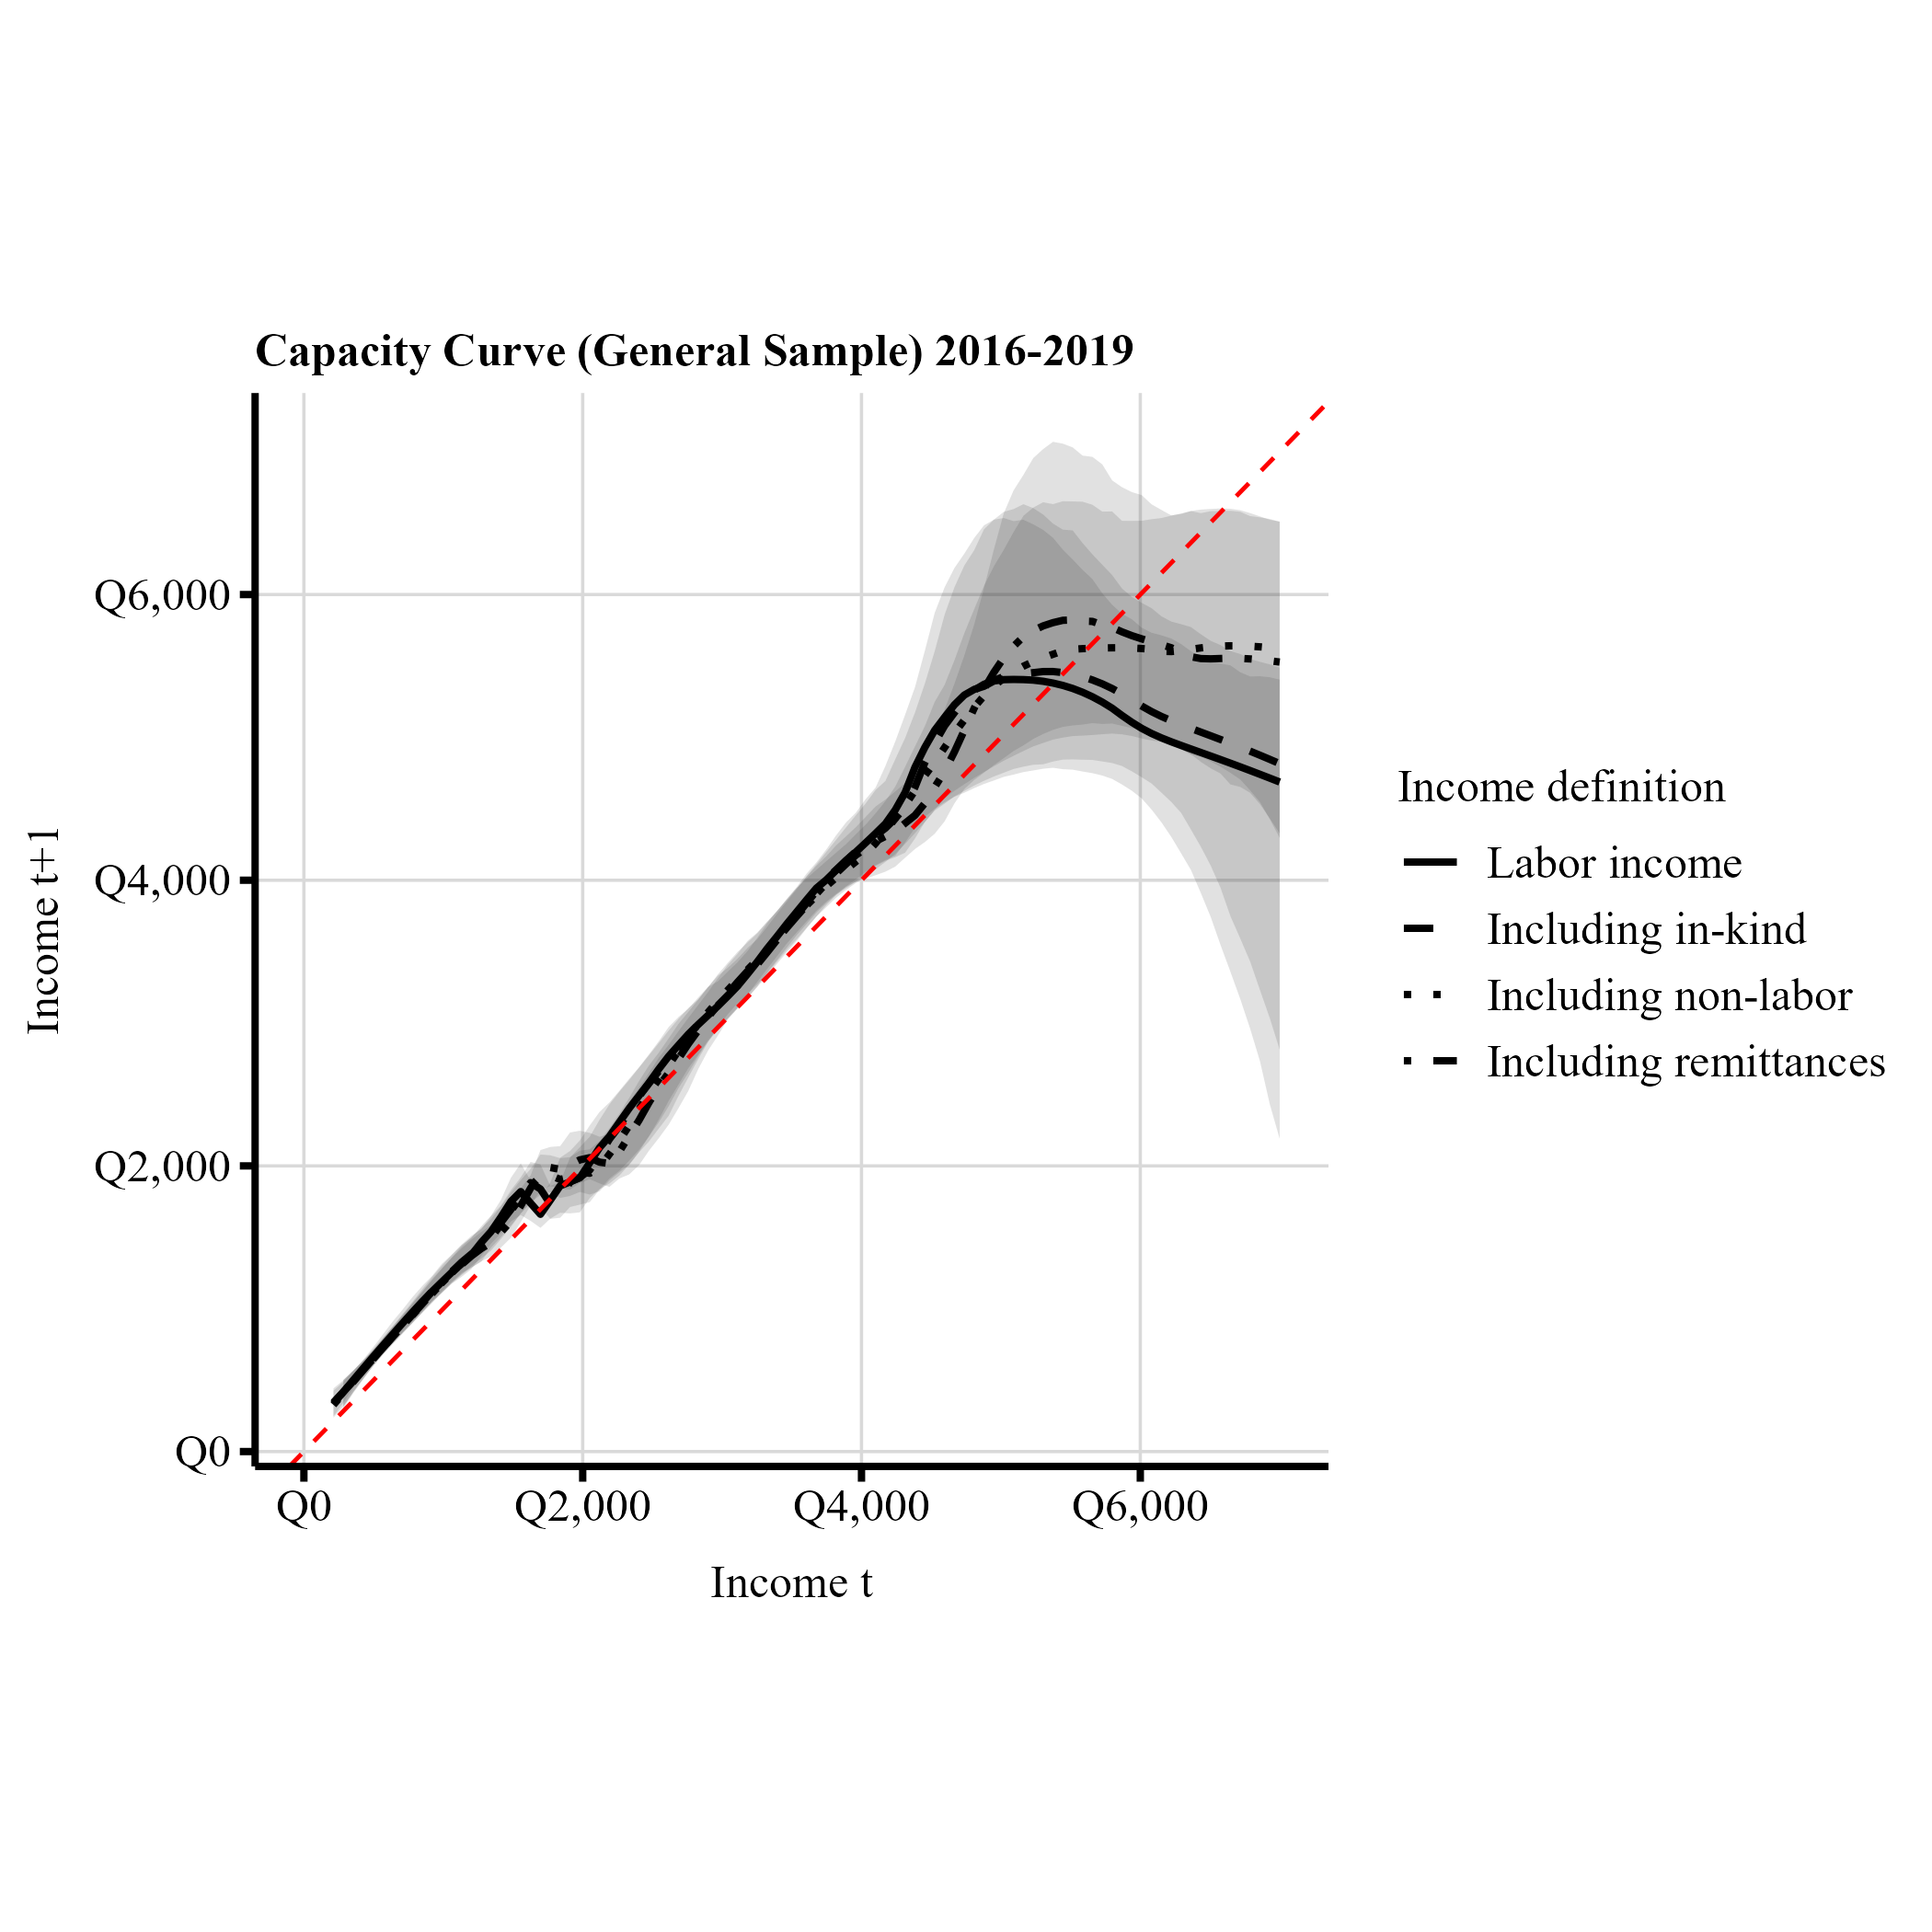
\includegraphics[trim={0.72bp 78.24bp 9.12bp 77.52bp},clip,width=0.90\linewidth,height=0.36\textheight,keepaspectratio]{figures/main-2016-2019-figure1.png}
\caption{Capacity curves: General sample, 2016-2019.}
\label{fig:main-2016-2019-1}
\end{figure}

\begin{figure}[!htbp]
\singlespacing
\centering
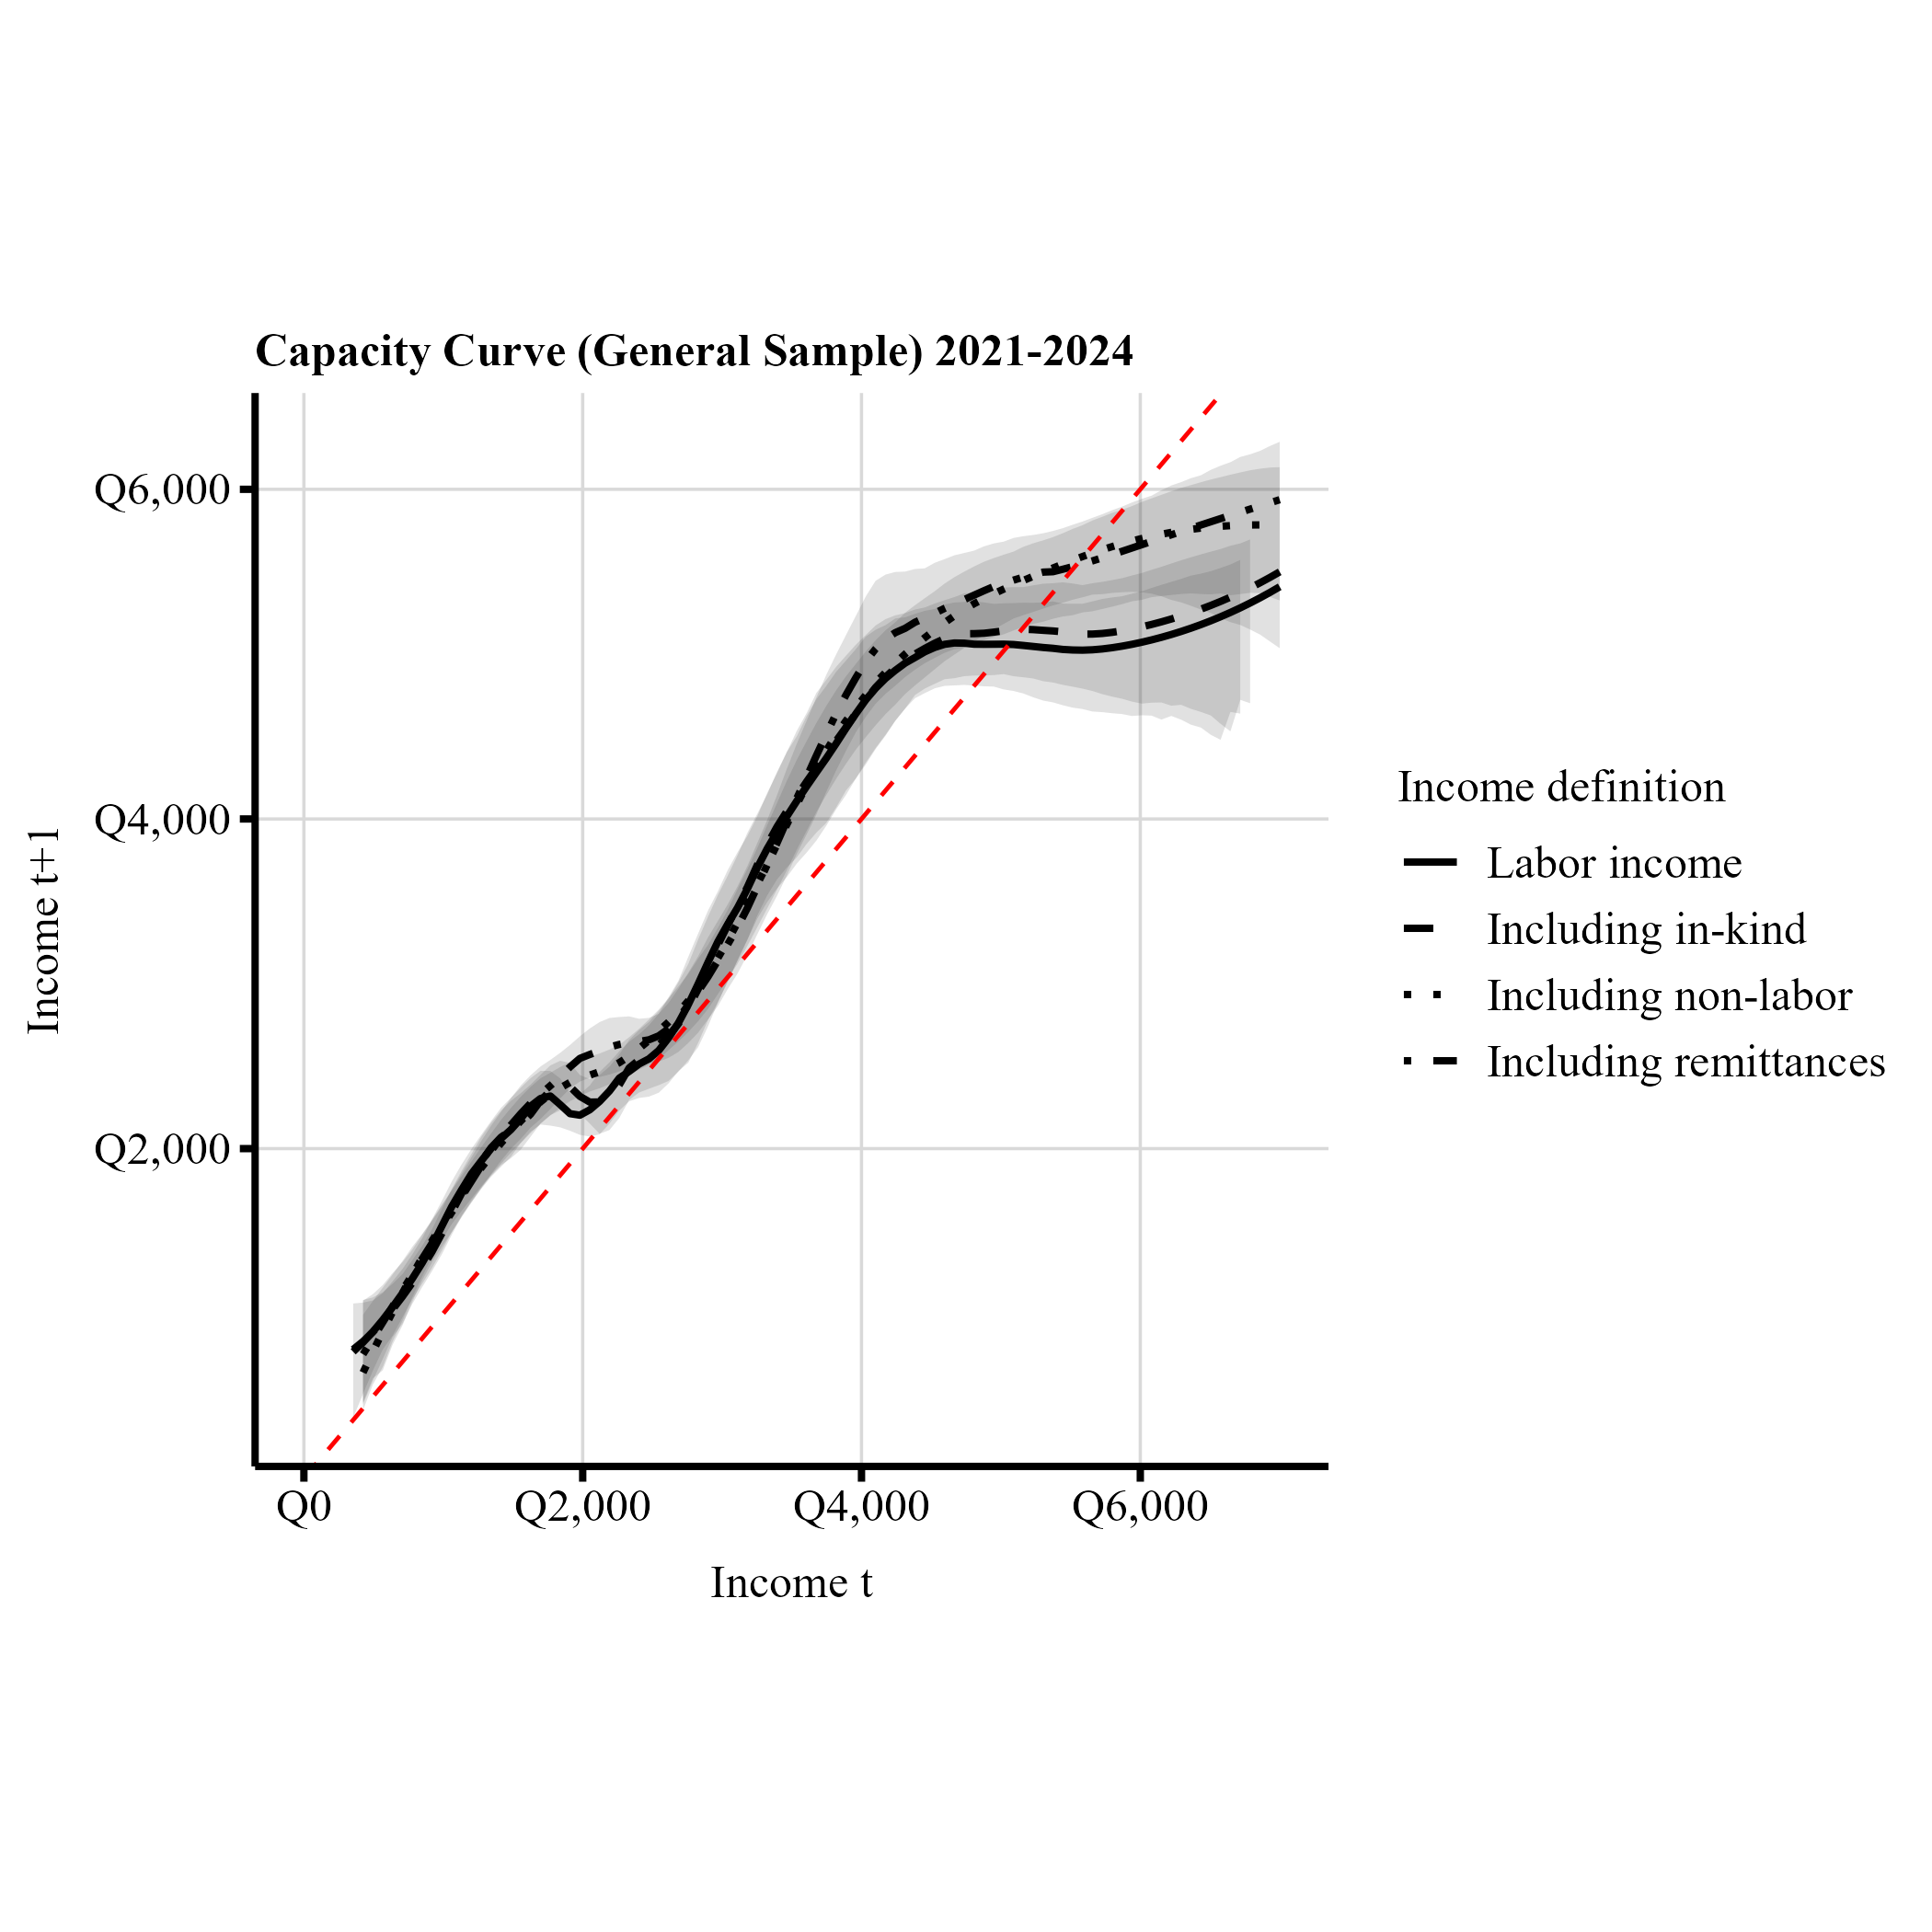
\includegraphics[trim={0.72bp 78.24bp 9.12bp 77.52bp},clip,width=0.90\linewidth,height=0.36\textheight,keepaspectratio]{figures/main-2021-2024-figure1.png}
\caption{Capacity curves: General sample, 2021-2024.}
\label{fig:main-2021-2024-1}
\end{figure}

\begin{figure}[!htbp]
\singlespacing
\centering
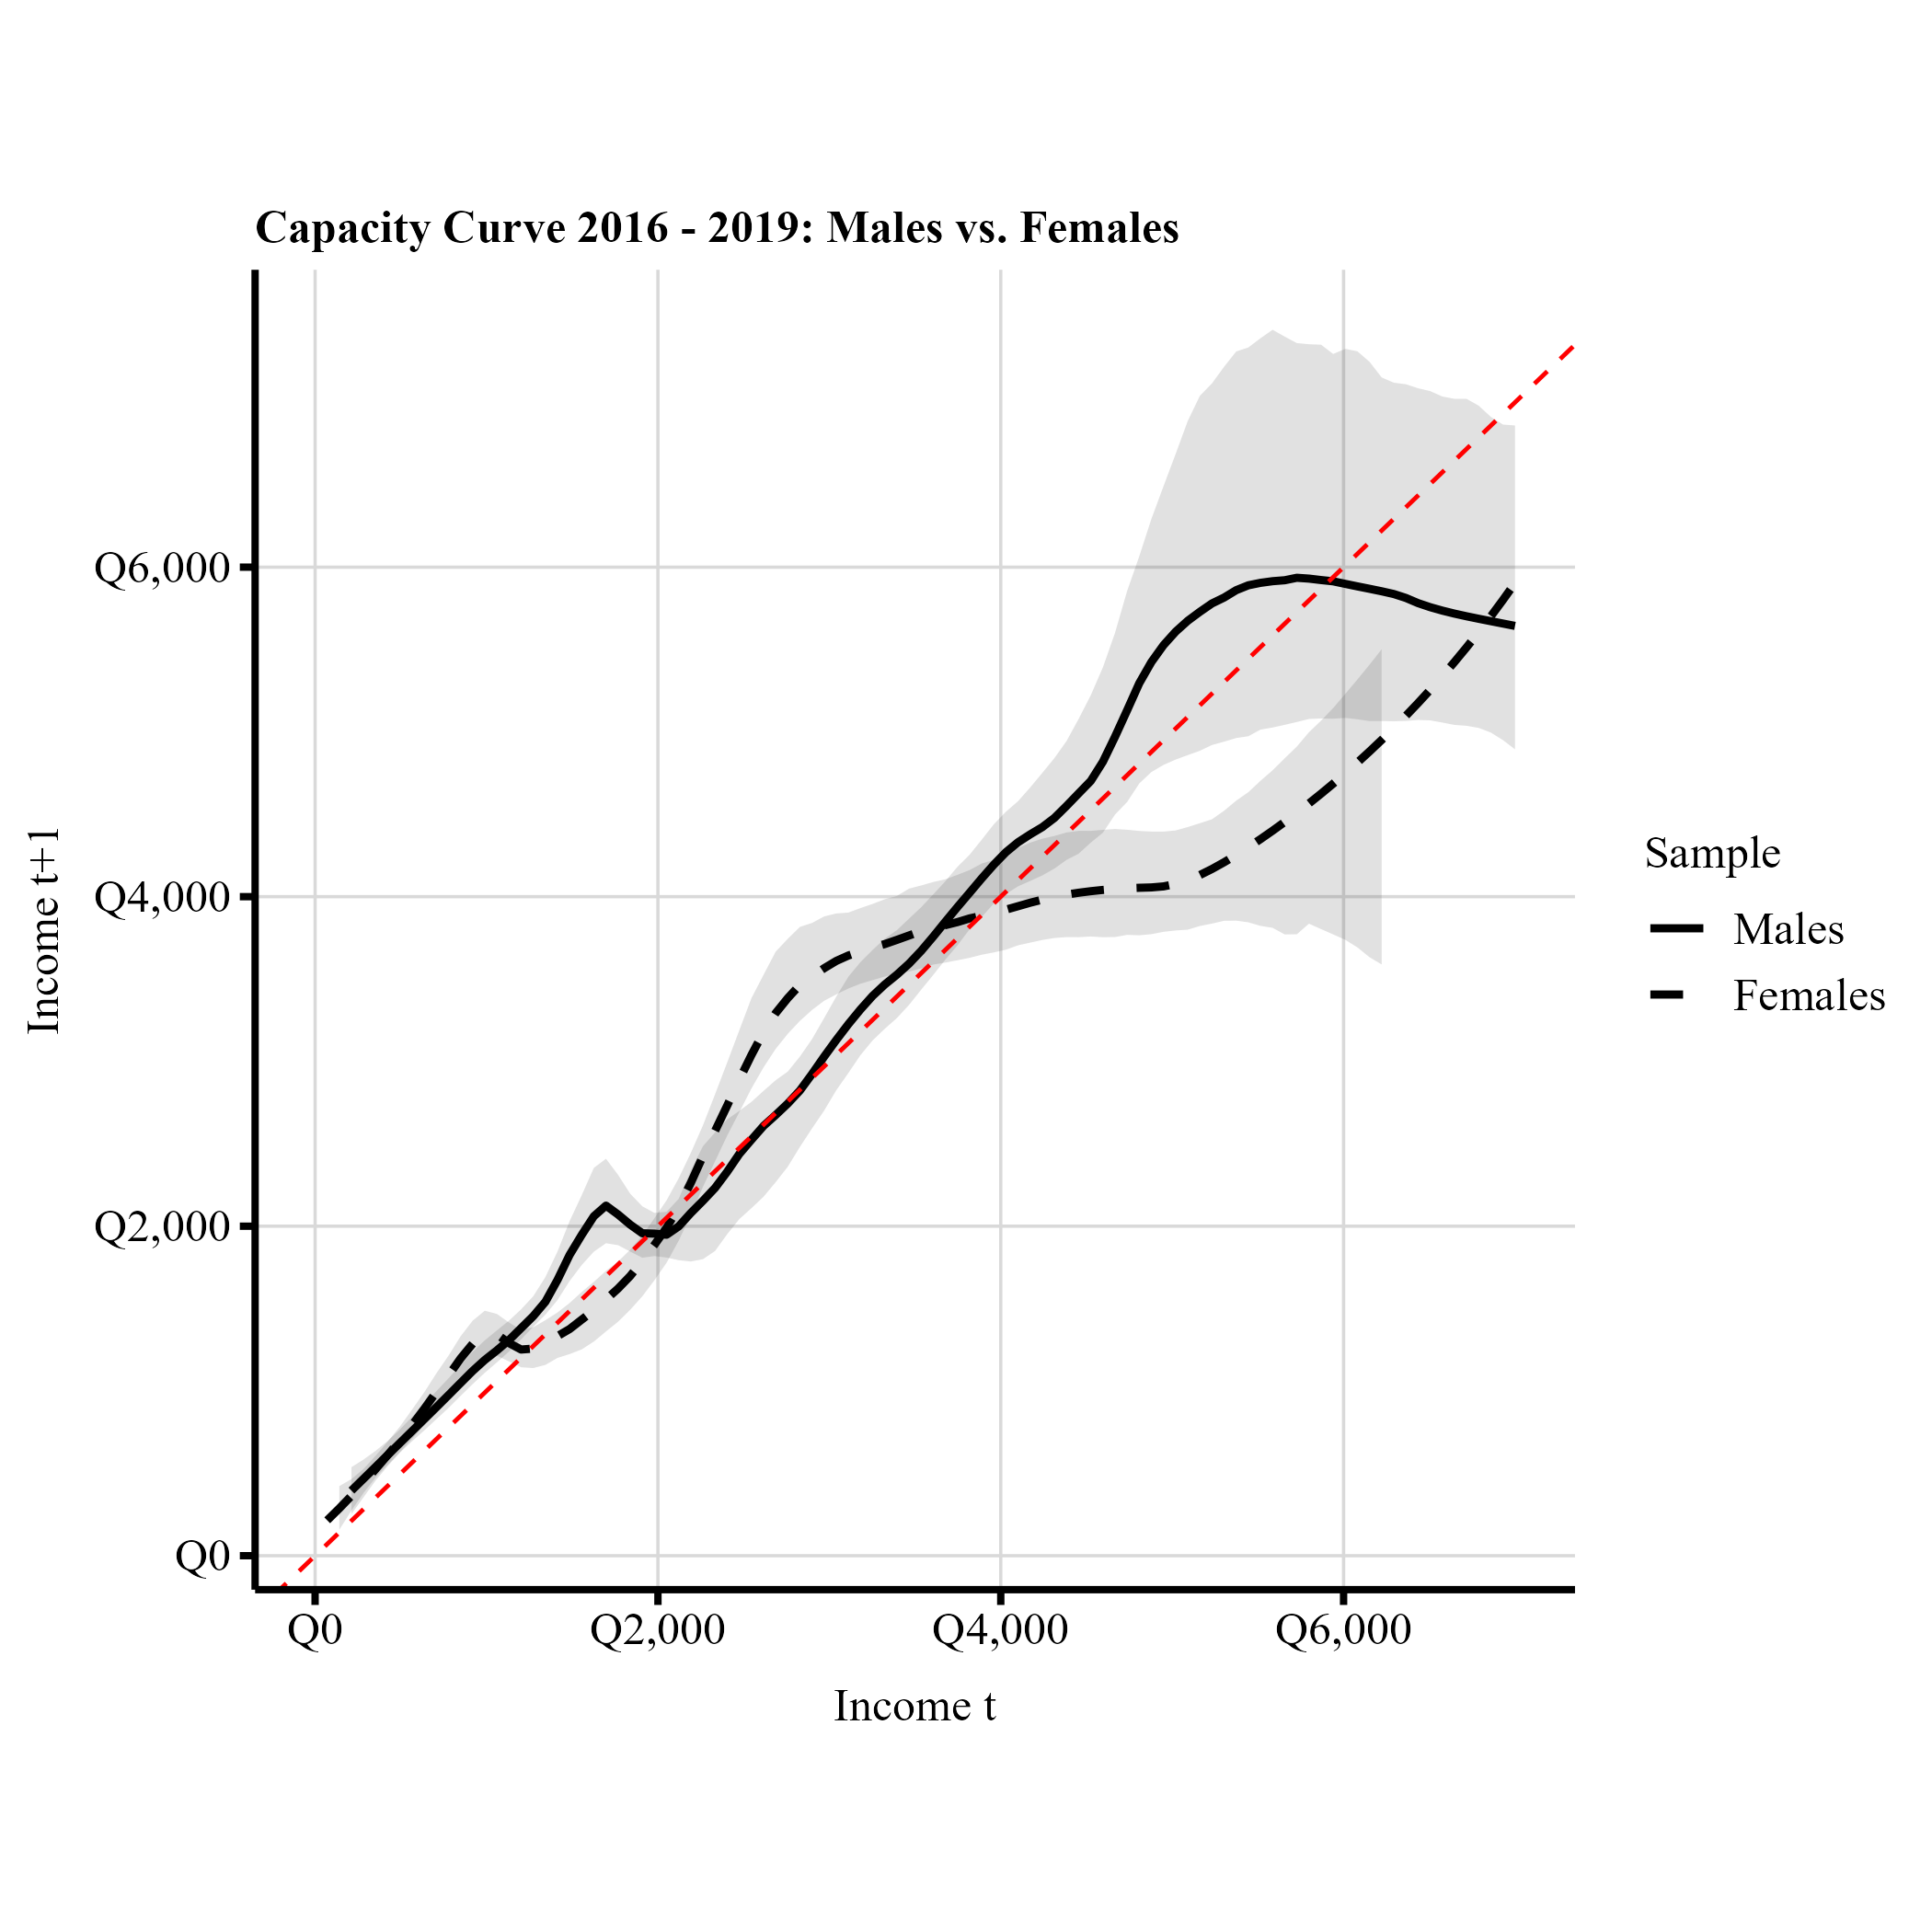
\includegraphics[trim={0.72bp 47.52bp 12.96bp 46.80bp},clip,width=0.90\linewidth,height=0.36\textheight,keepaspectratio]{figures/main-2016-2019-figure2.png}
\caption{Capacity curves: Males and females, 2016-2019.}
\label{fig:main-2016-2019-2}
\end{figure}

\begin{figure}[!htbp]
\singlespacing
\centering
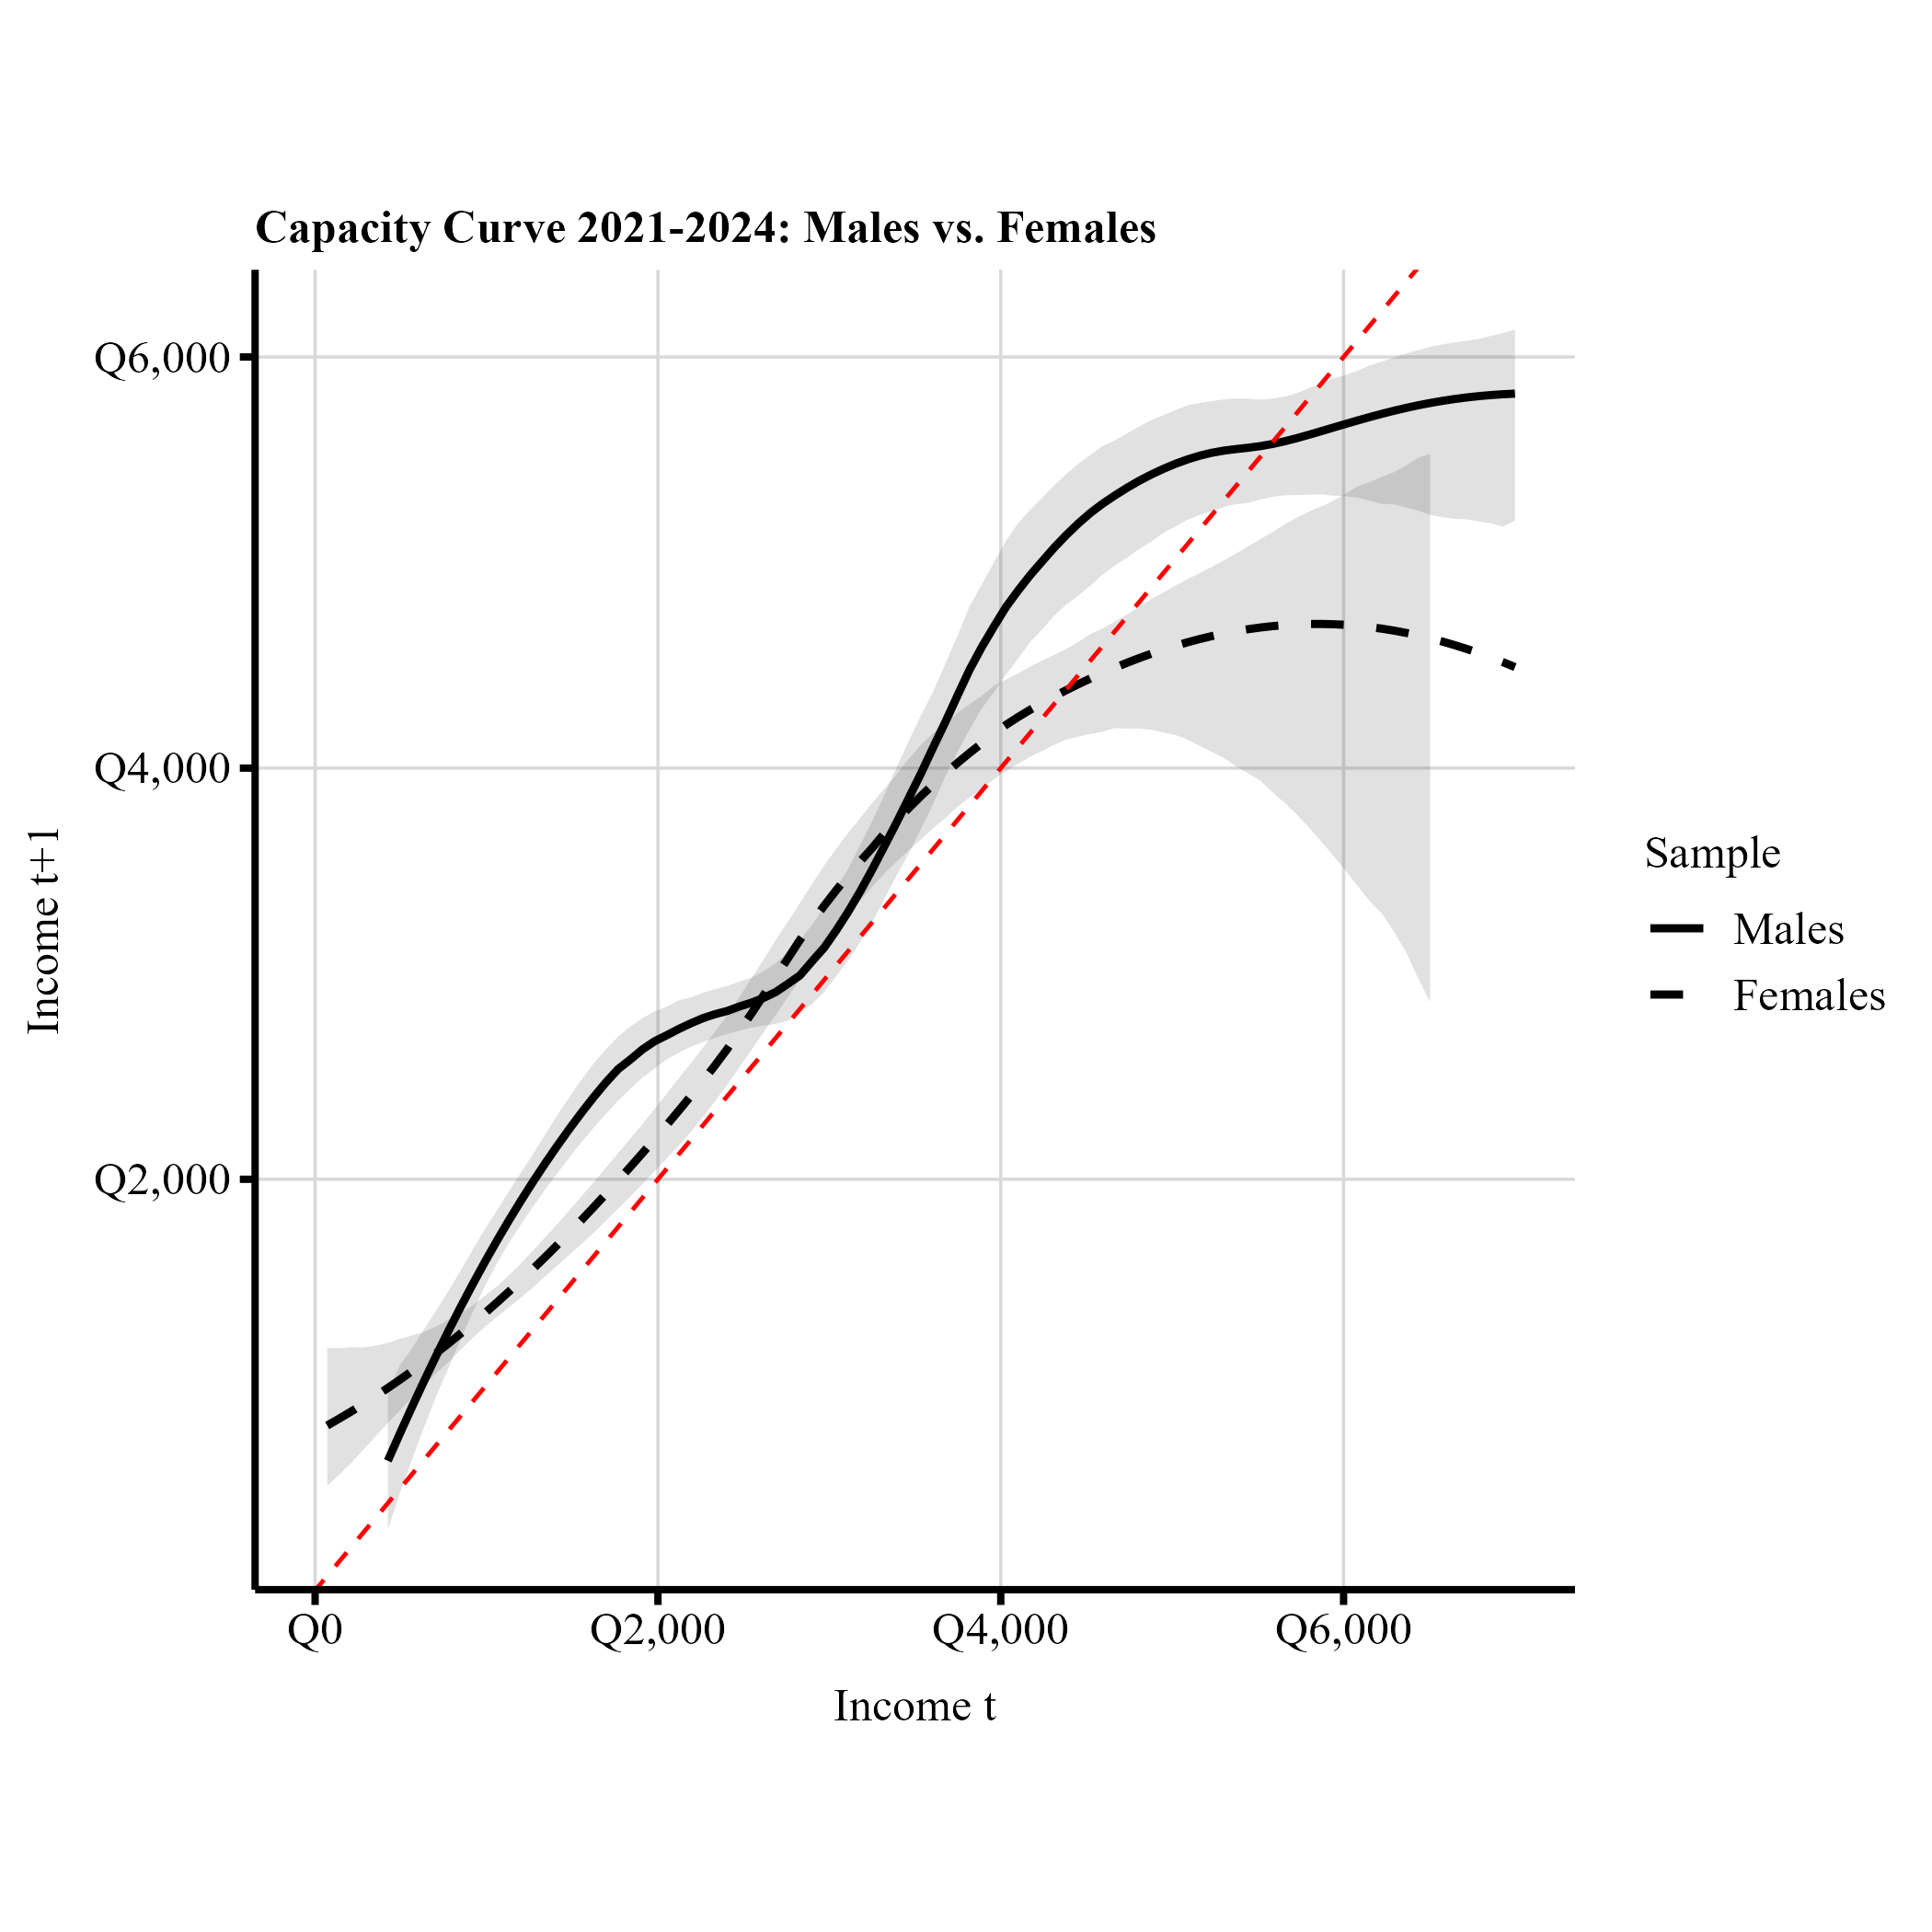
\includegraphics[trim={0.72bp 47.52bp 12.96bp 46.80bp},clip,width=0.90\linewidth,height=0.36\textheight,keepaspectratio]{figures/main-2021-2024-figure2.png}
\caption{Capacity curves: Males and females, 2021-2024.}
\label{fig:main-2021-2024-2}
\end{figure}

\begin{figure}[!htbp]
\singlespacing
\centering
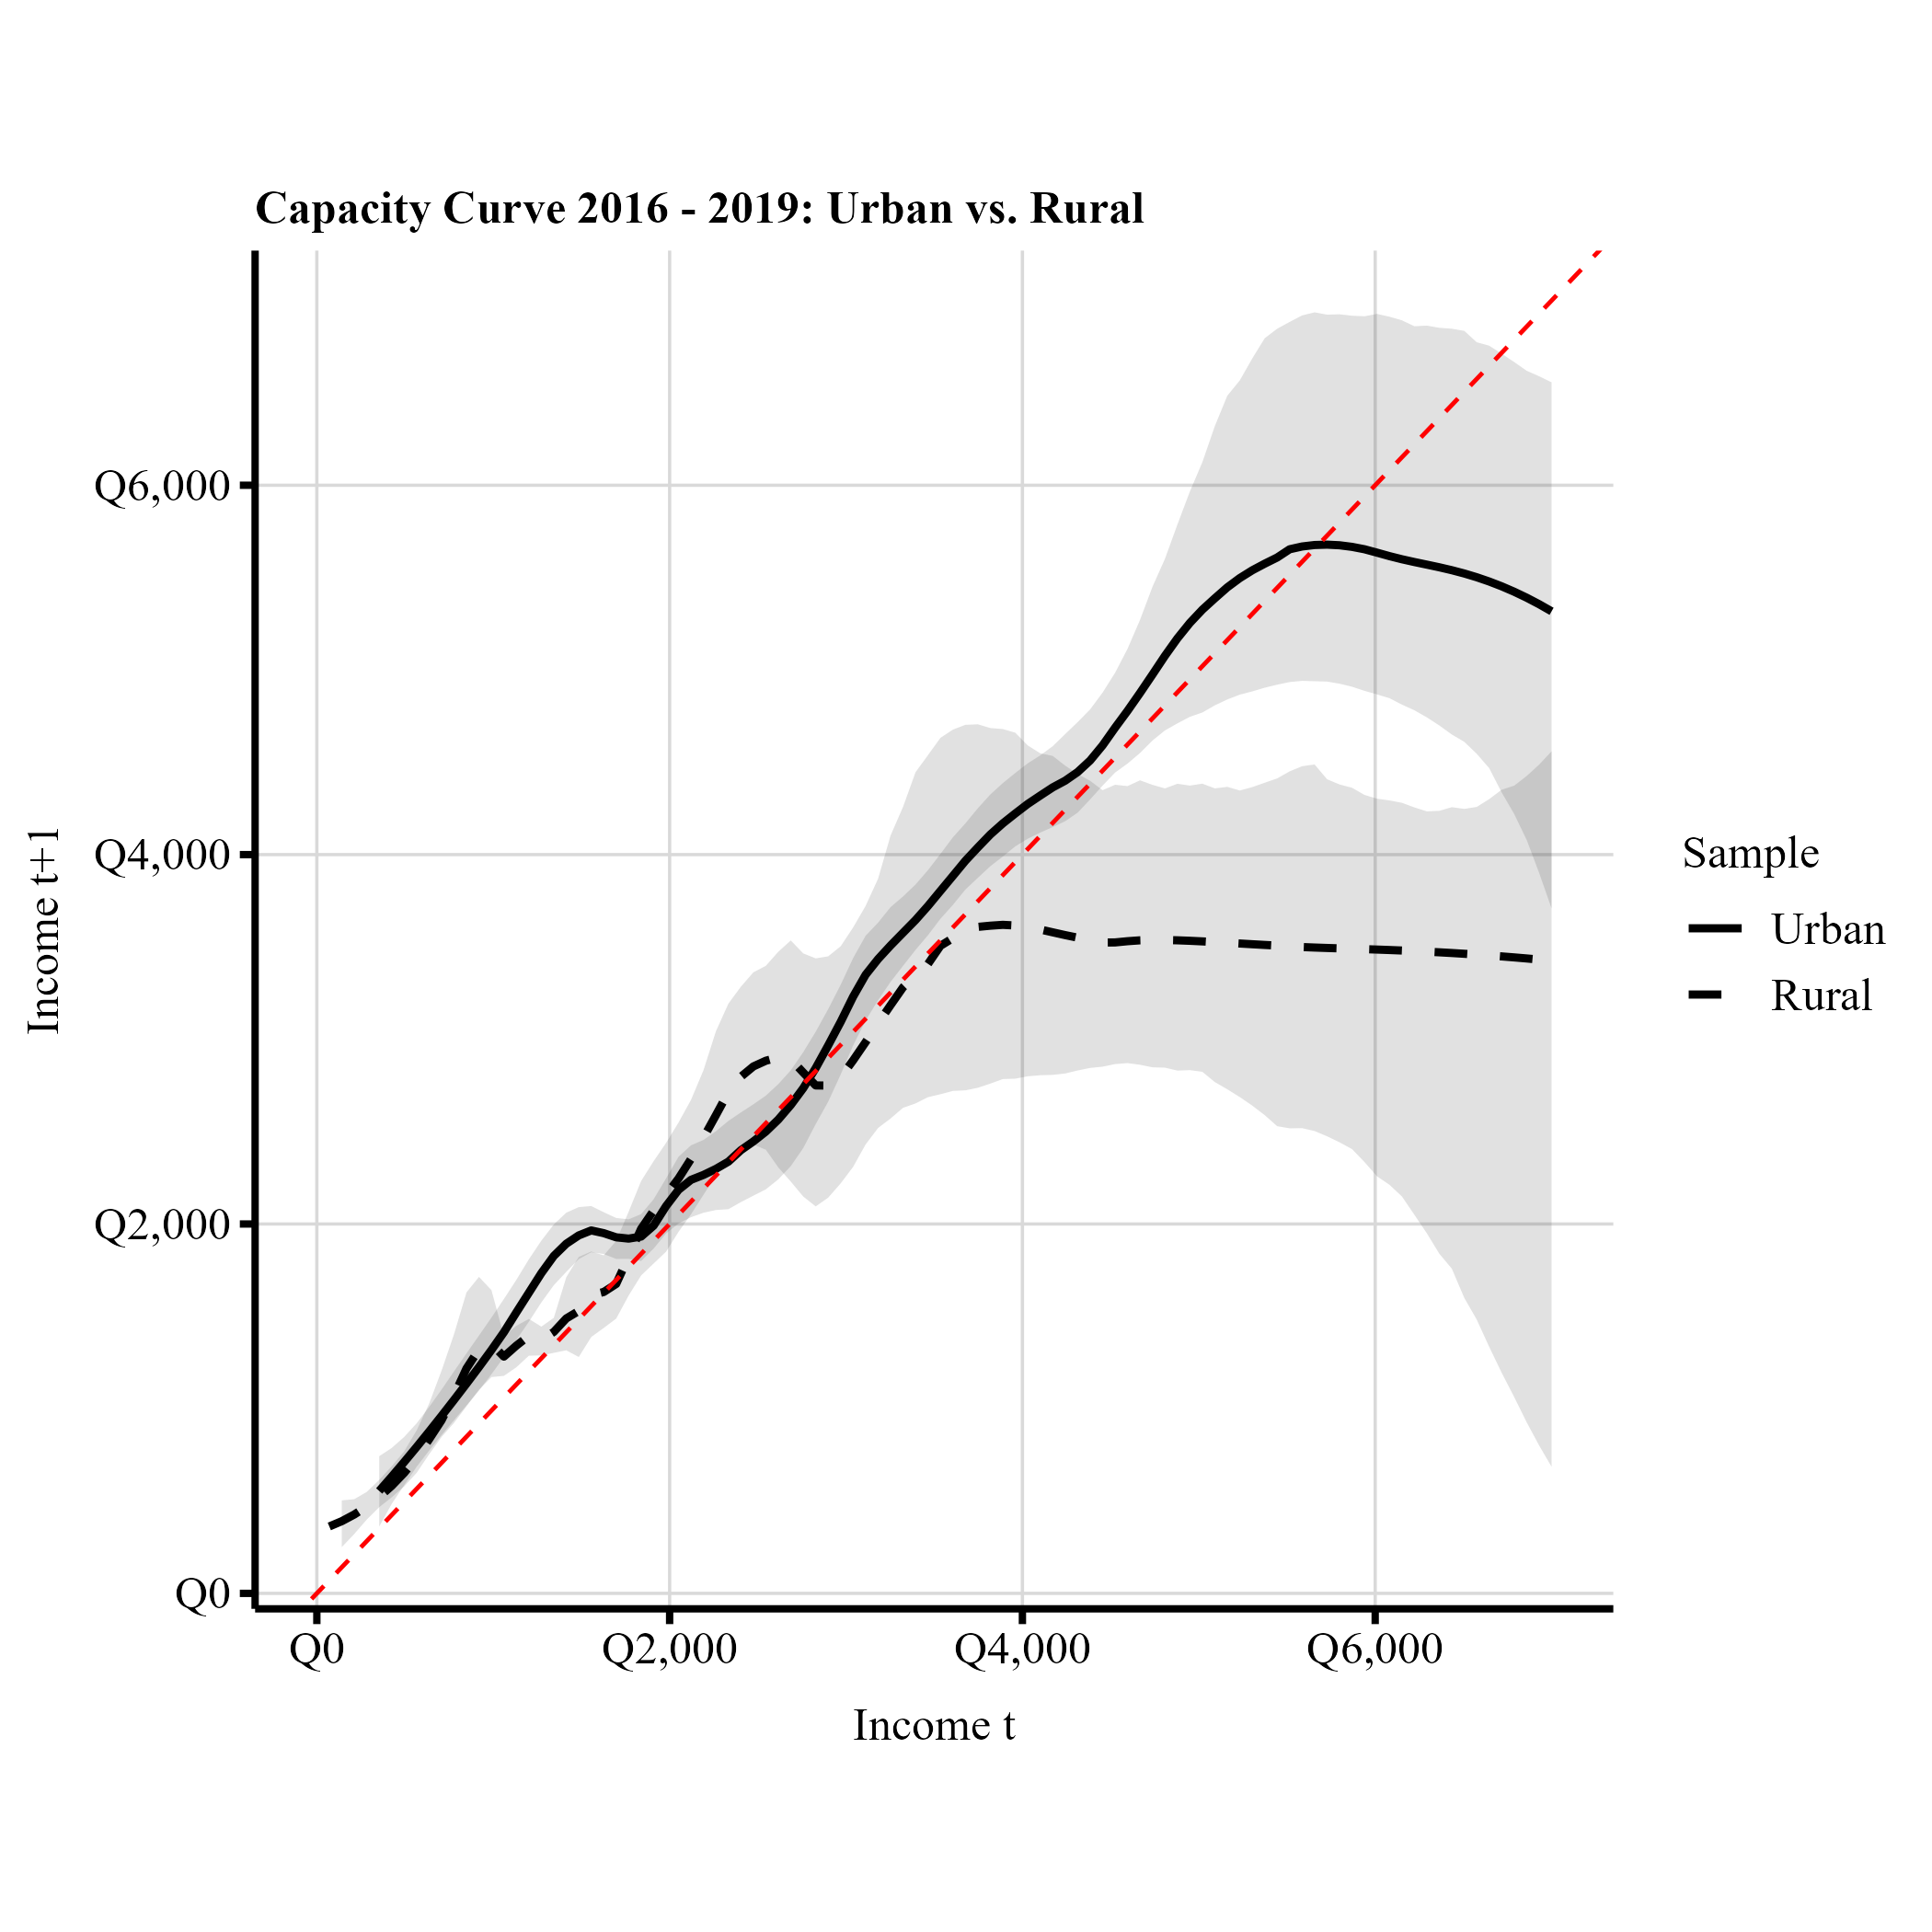
\includegraphics[trim={0.72bp 39.84bp 5.28bp 39.12bp},clip,width=0.90\linewidth,height=0.36\textheight,keepaspectratio]{figures/main-2016-2019-figure3.png}
\caption{Capacity curves: Urban and rural populations, 2016-2019.}
\label{fig:main-2016-2019-3}
\end{figure}

\begin{figure}[!htbp]
\singlespacing
\centering
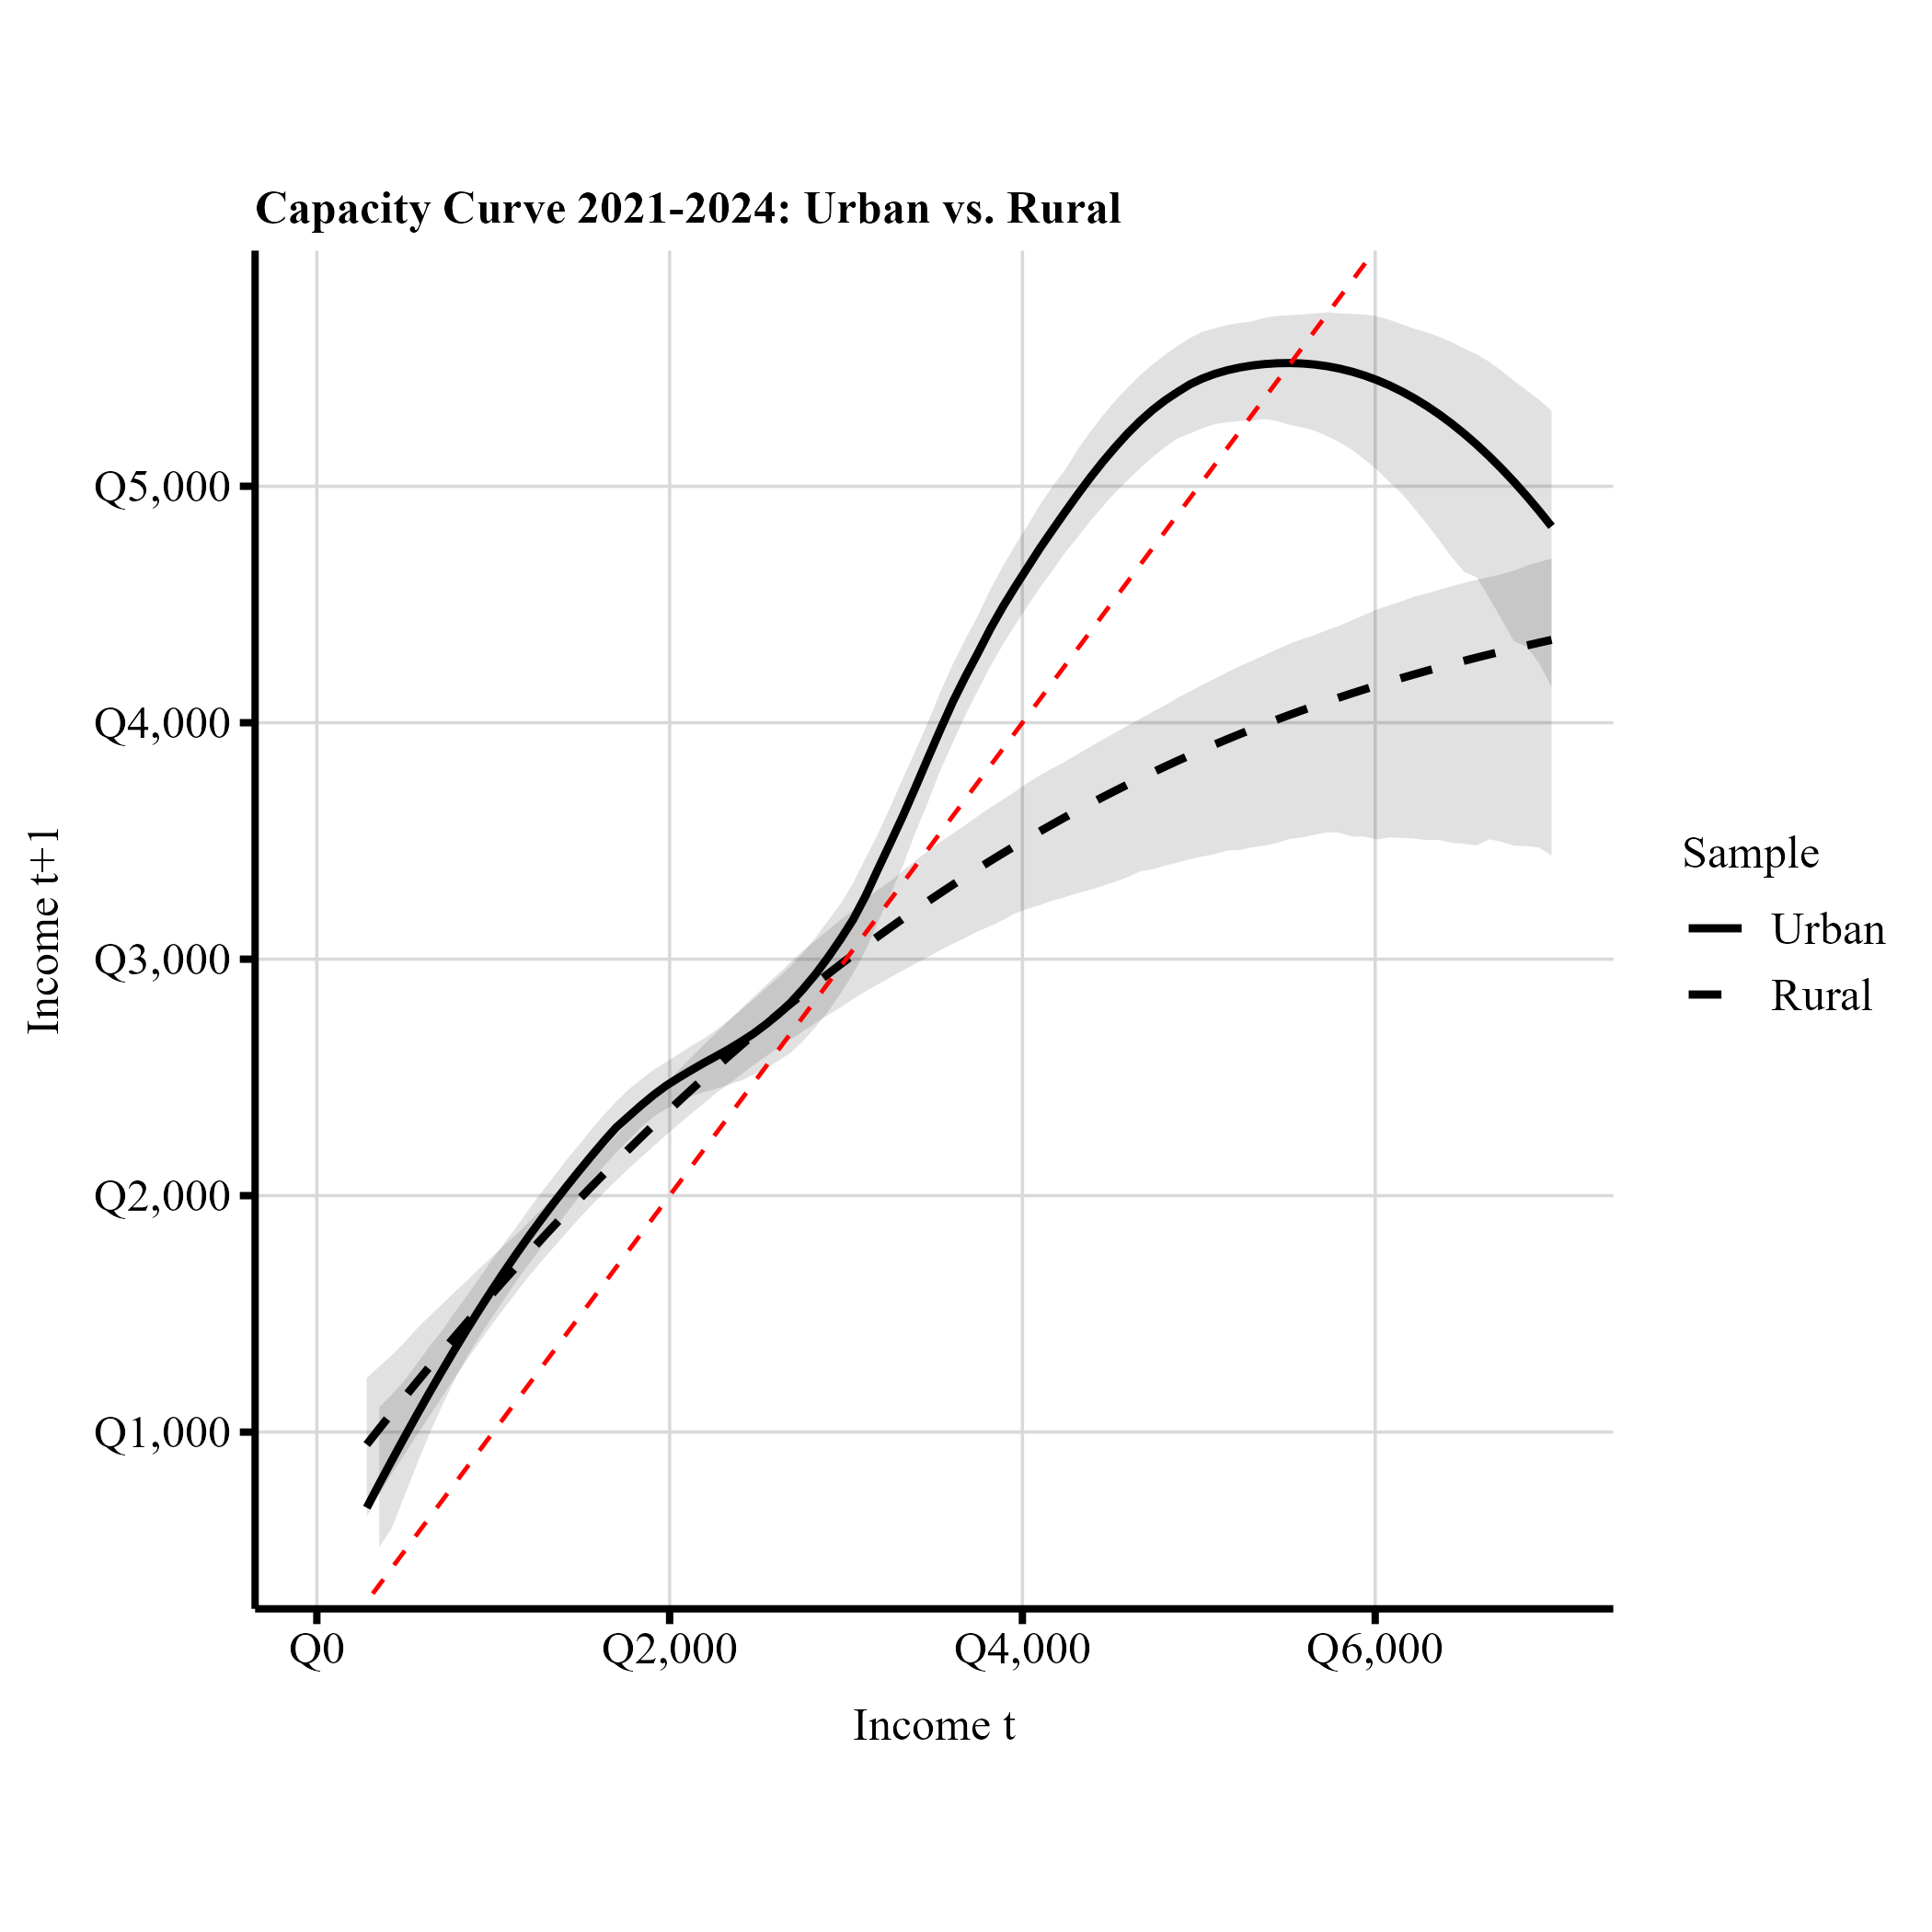
\includegraphics[trim={0.72bp 39.84bp 5.28bp 39.12bp},clip,width=0.90\linewidth,height=0.36\textheight,keepaspectratio]{figures/main-2021-2024-figure3.png}
\caption{Capacity curves: Urban and rural populations, 2021-2024.}
\label{fig:main-2021-2024-3}
\end{figure}

\begin{figure}[!htbp]
\singlespacing
\centering
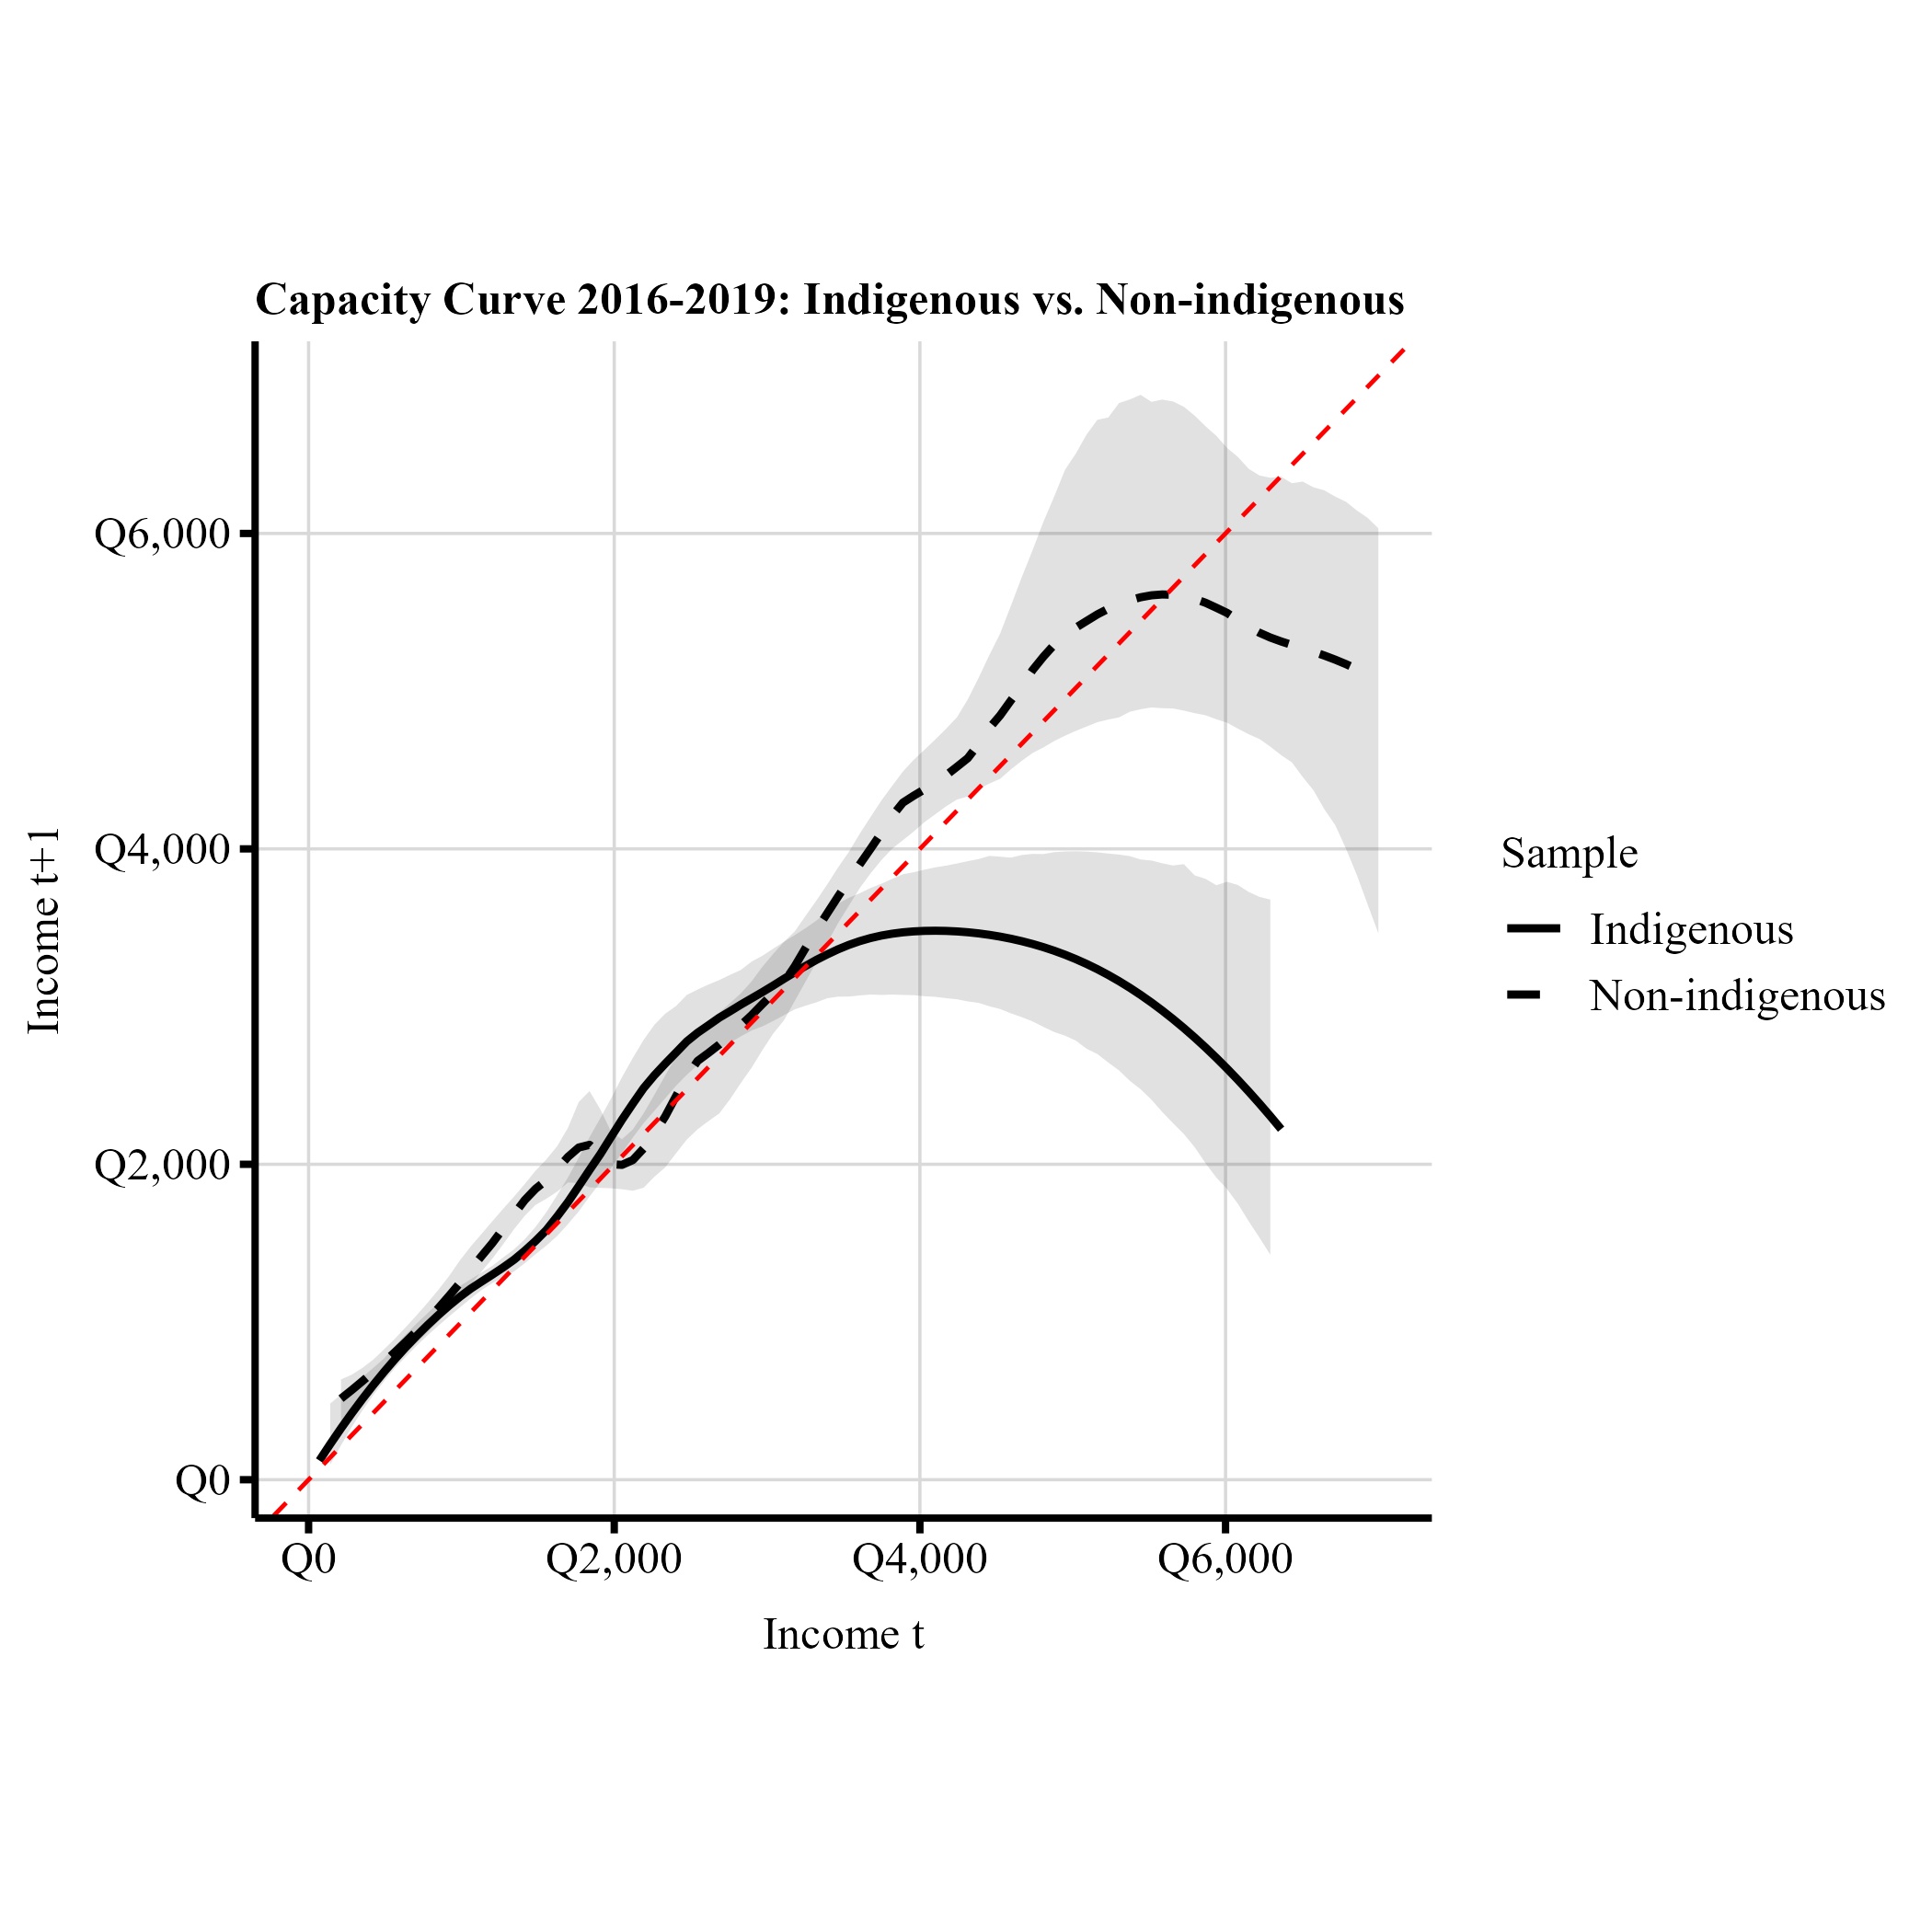
\includegraphics[trim={0.72bp 66.72bp 12.96bp 66.00bp},clip,width=0.90\linewidth,height=0.36\textheight,keepaspectratio]{figures/main-2016-2019-figure4.png}
\caption{Capacity curves: Indigenous and non-indigenous populations, 2016-2019.}
\label{fig:main-2016-2019-4}
\end{figure}

\begin{figure}[!htbp]
\singlespacing
\centering
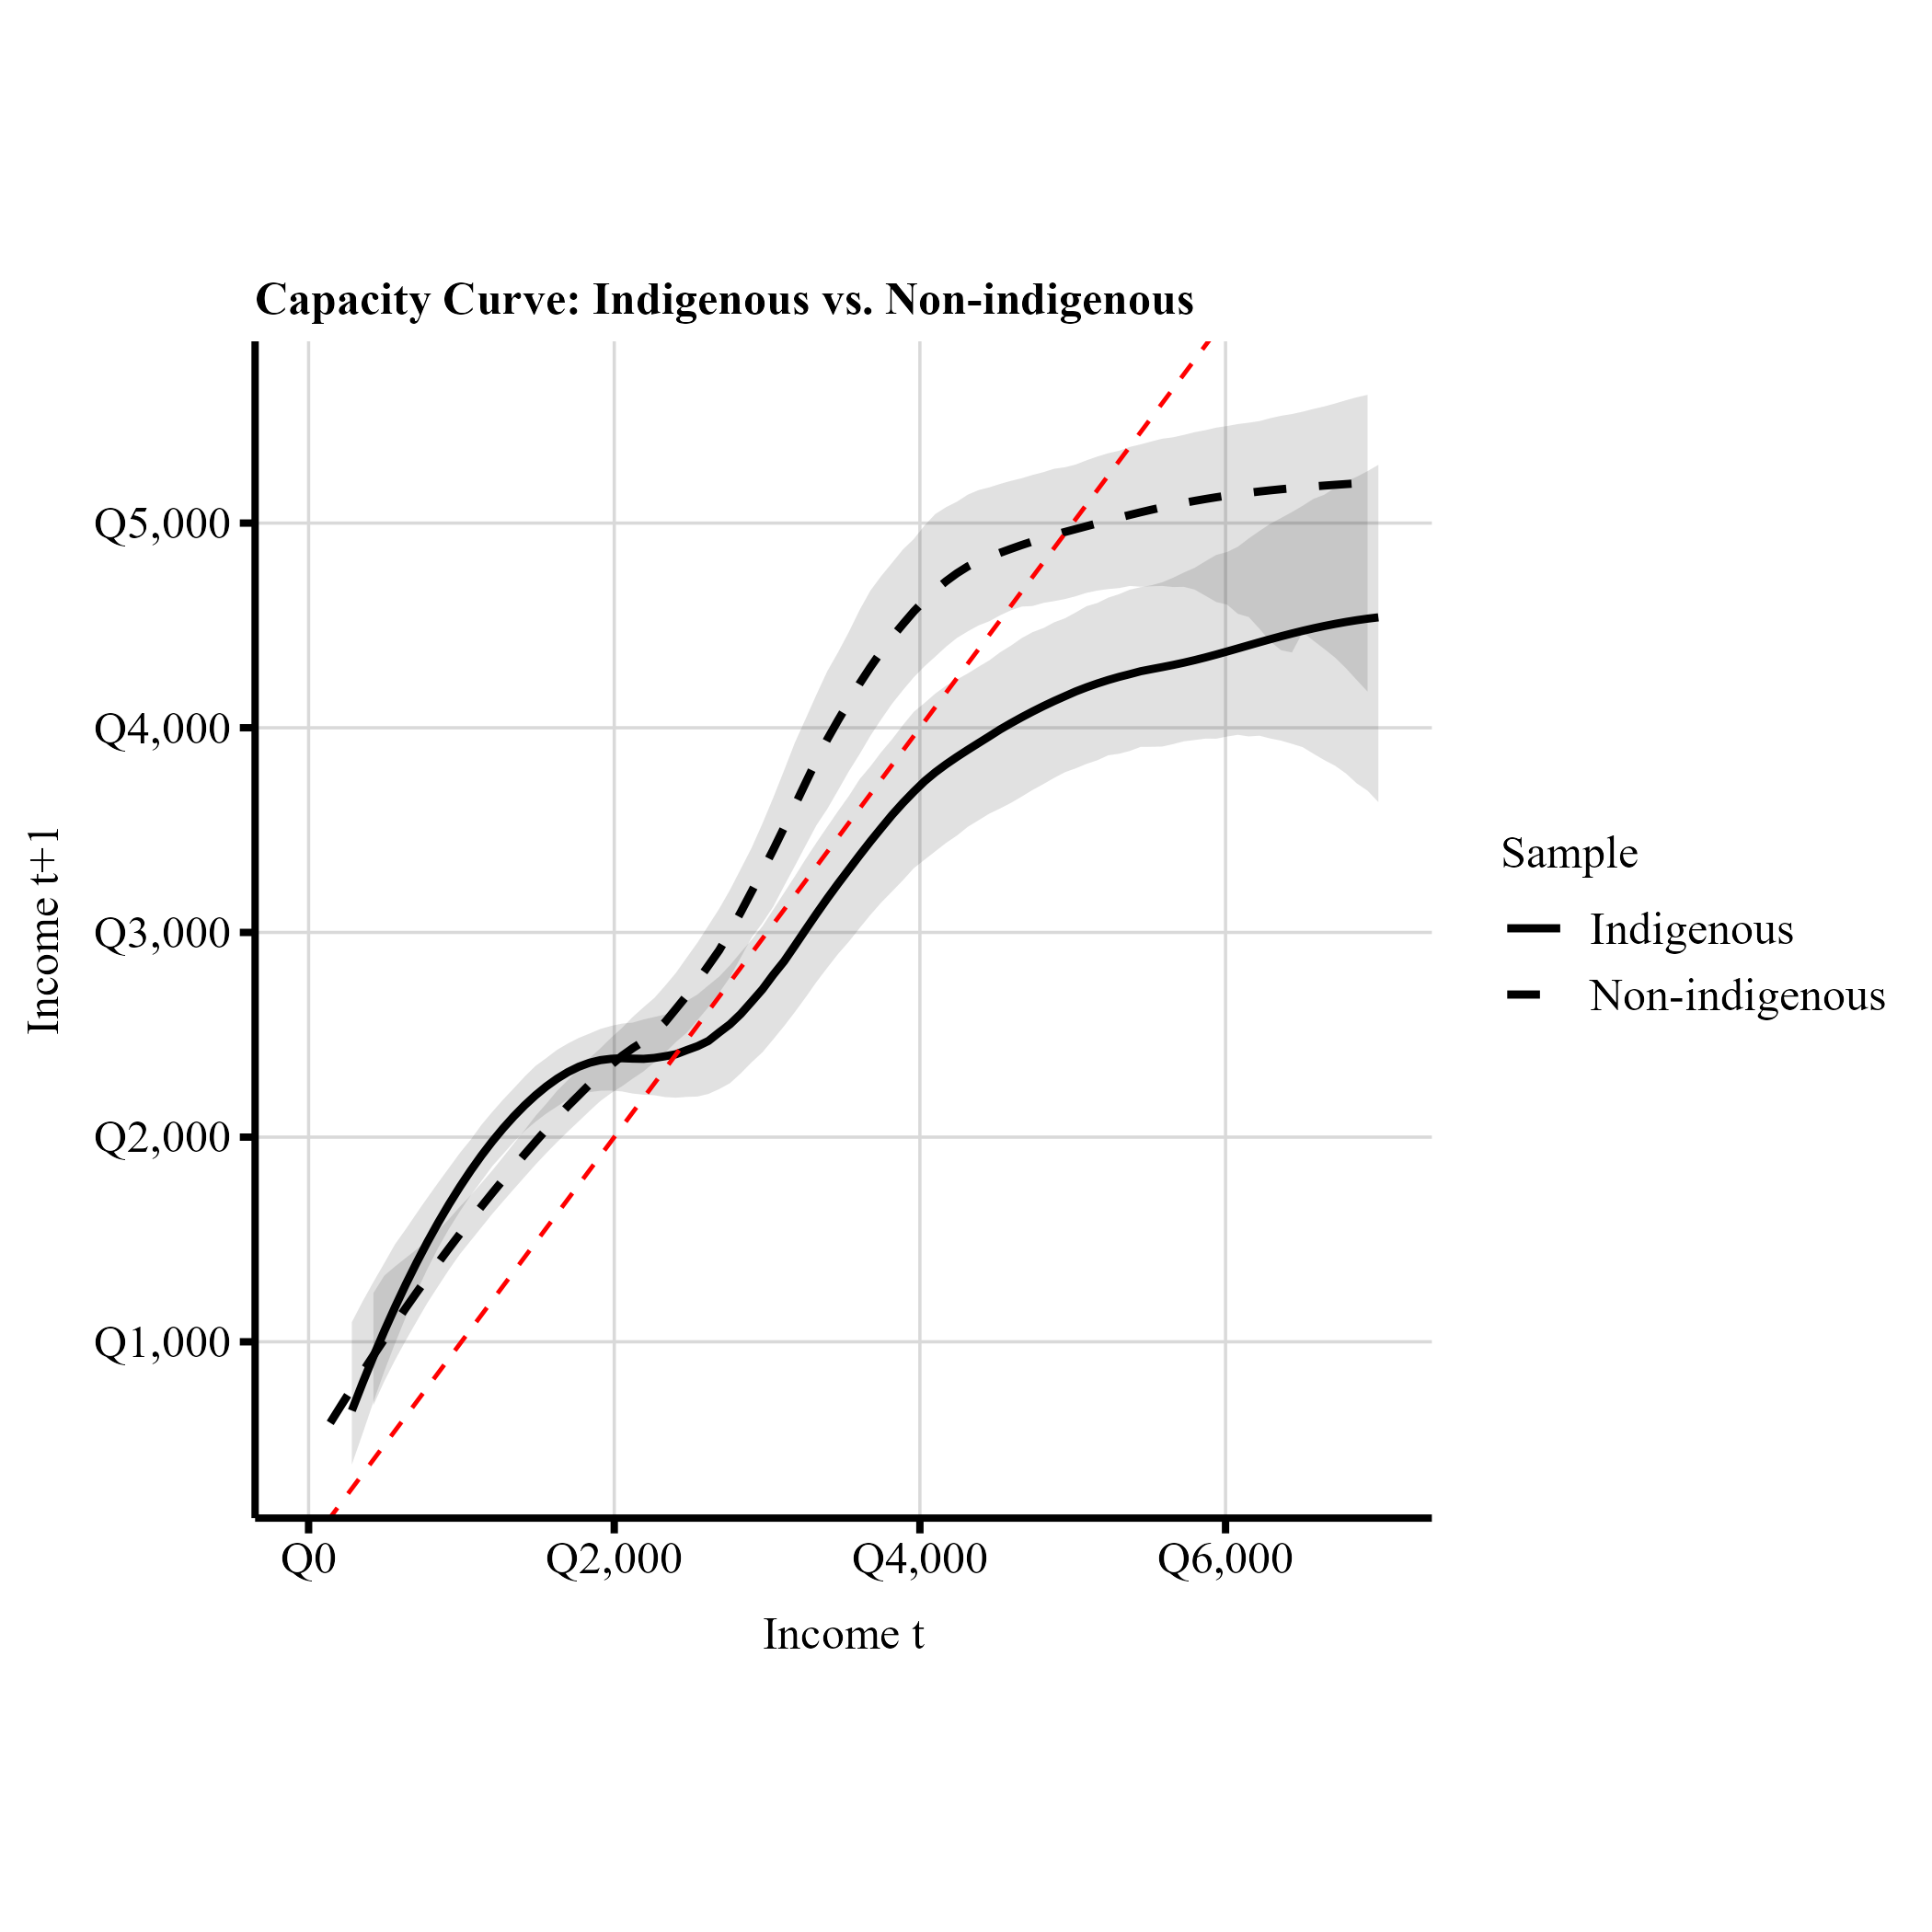
\includegraphics[trim={0.72bp 66.72bp 12.96bp 66.00bp},clip,width=0.90\linewidth,height=0.36\textheight,keepaspectratio]{figures/main-2021-2024-figure4.png}
\caption{Capacity curves: Indigenous and non-indigenous populations, 2021-2024.}
\label{fig:main-2021-2024-4}
\end{figure}

\begin{figure}[!htbp]
\singlespacing
\centering
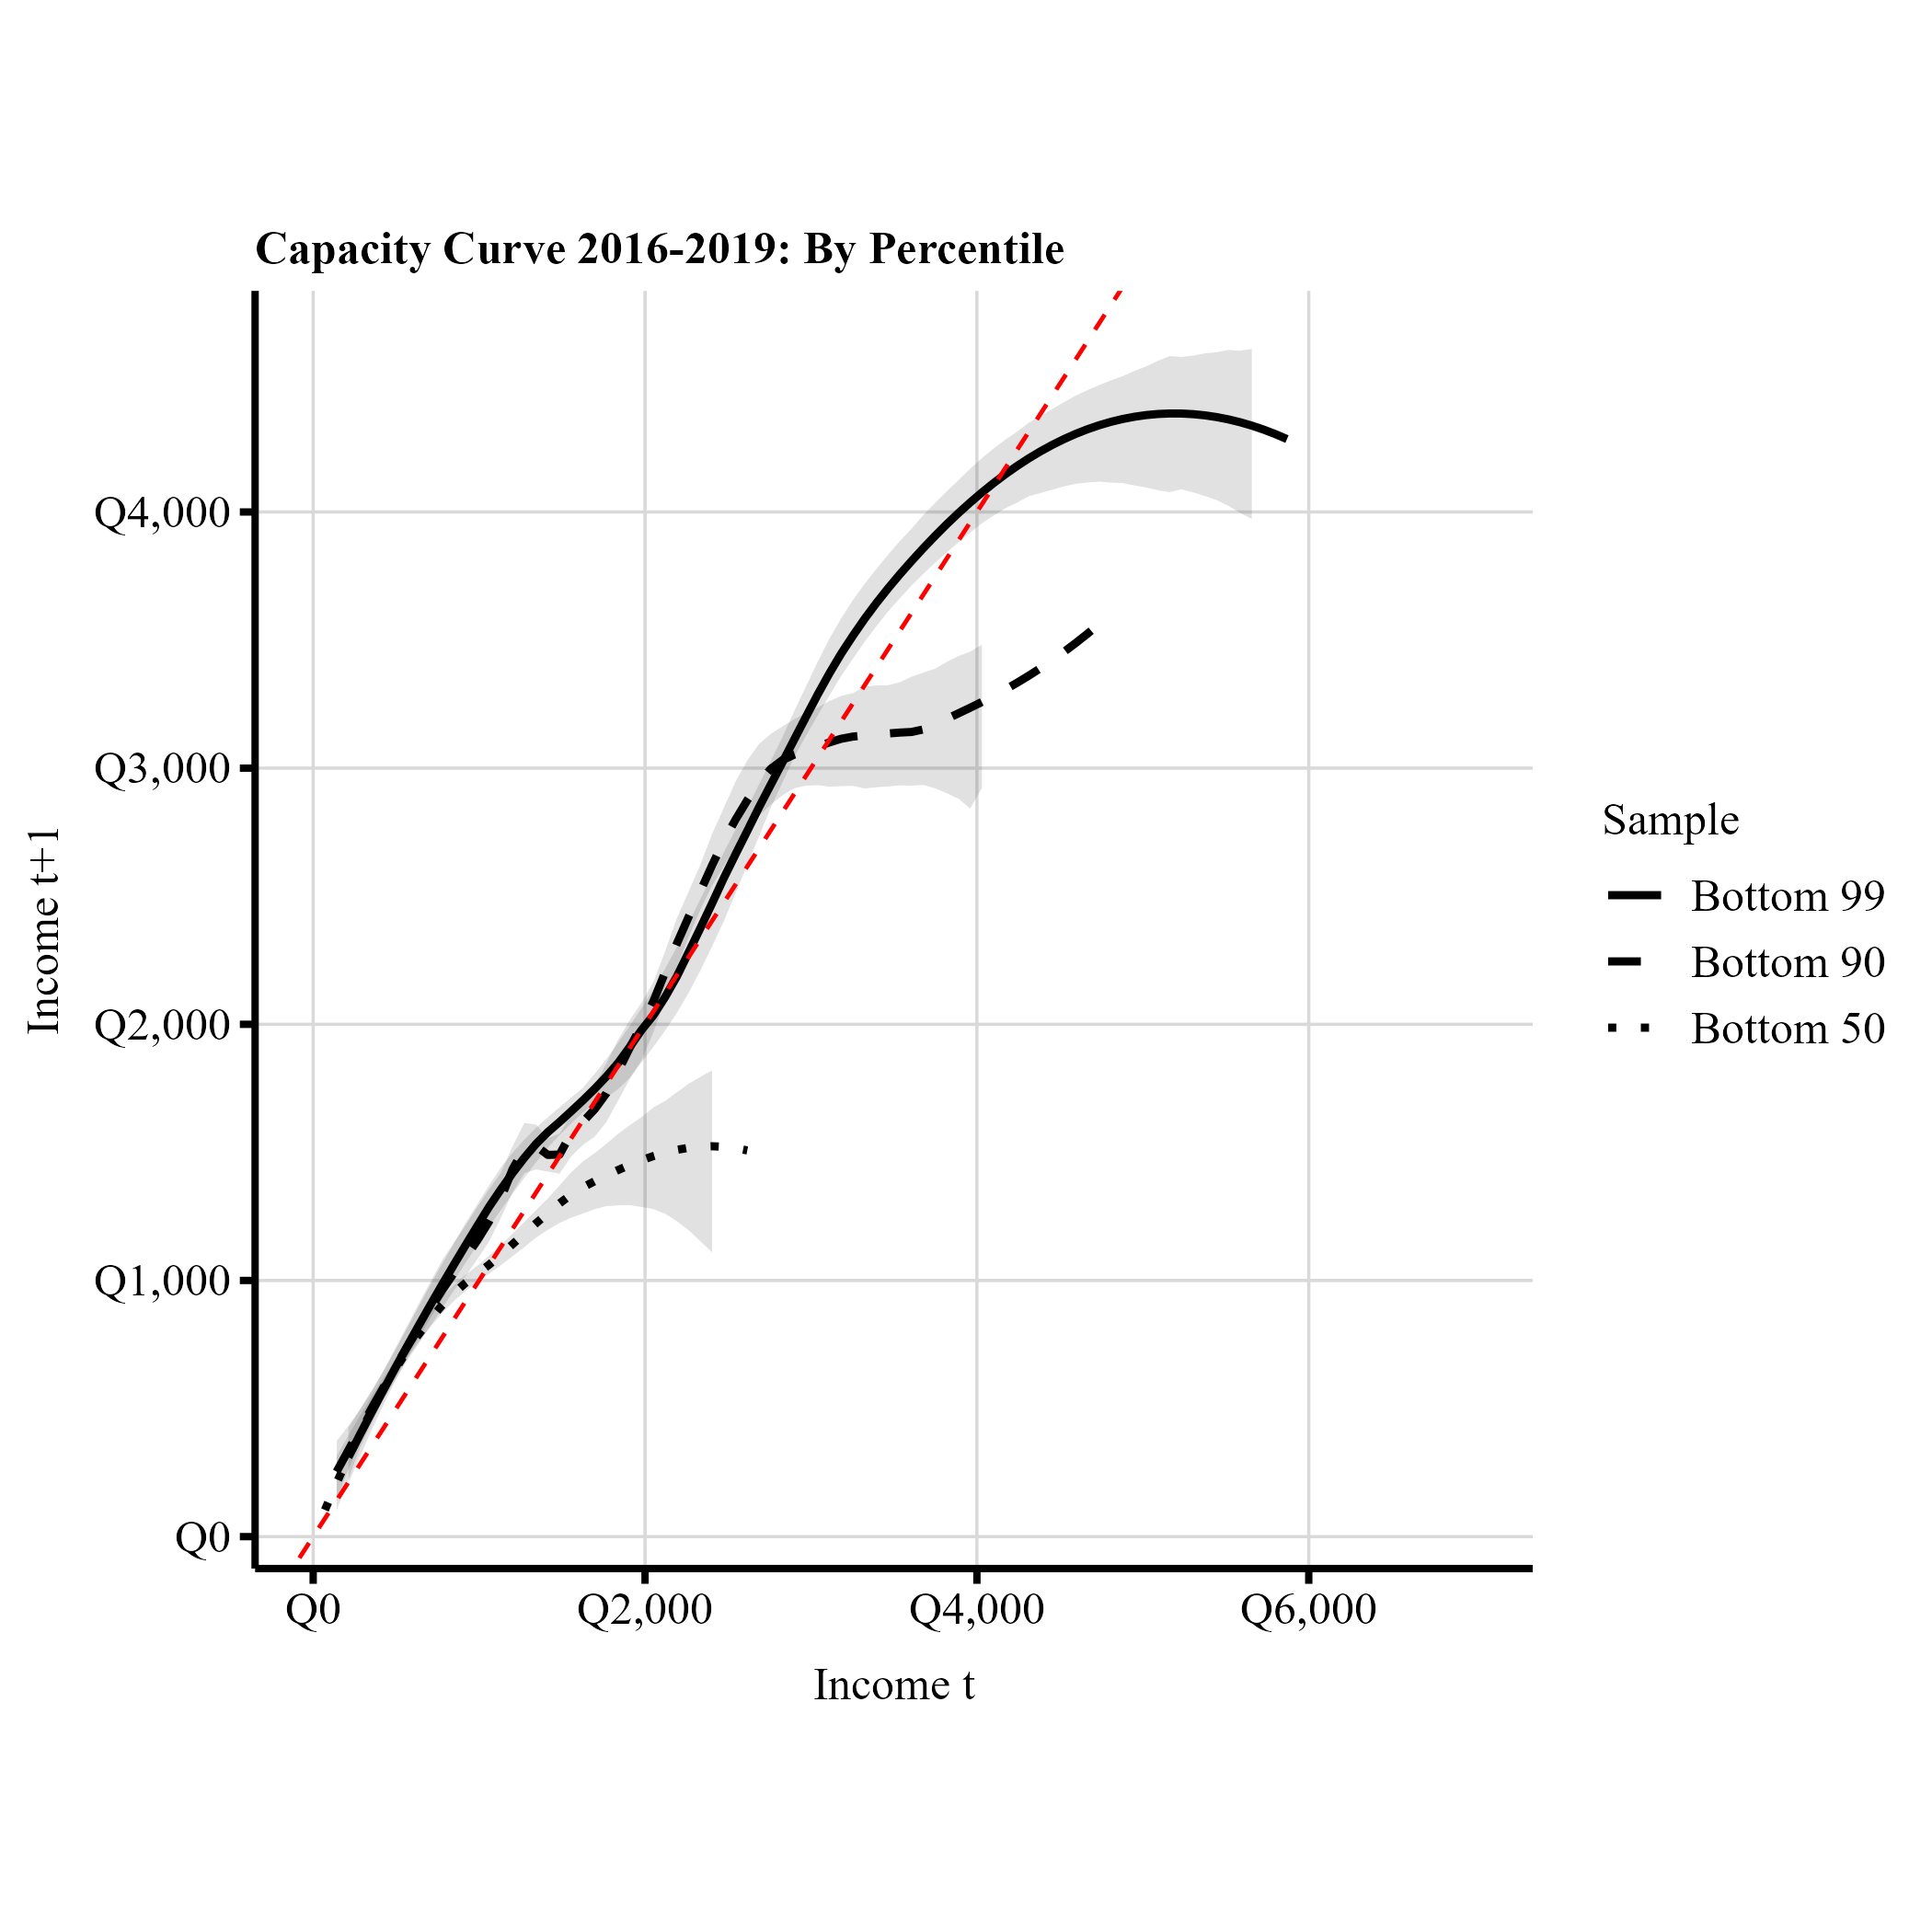
\includegraphics[trim={0.72bp 51.36bp 5.28bp 50.64bp},clip,width=0.90\linewidth,height=0.36\textheight,keepaspectratio]{figures/main-2016-2019-figure5.png}
\caption{Capacity curves: Income percentiles, 2016-2019.}
\label{fig:main-2016-2019-5}
\end{figure}

\begin{figure}[!htbp]
\singlespacing
\centering
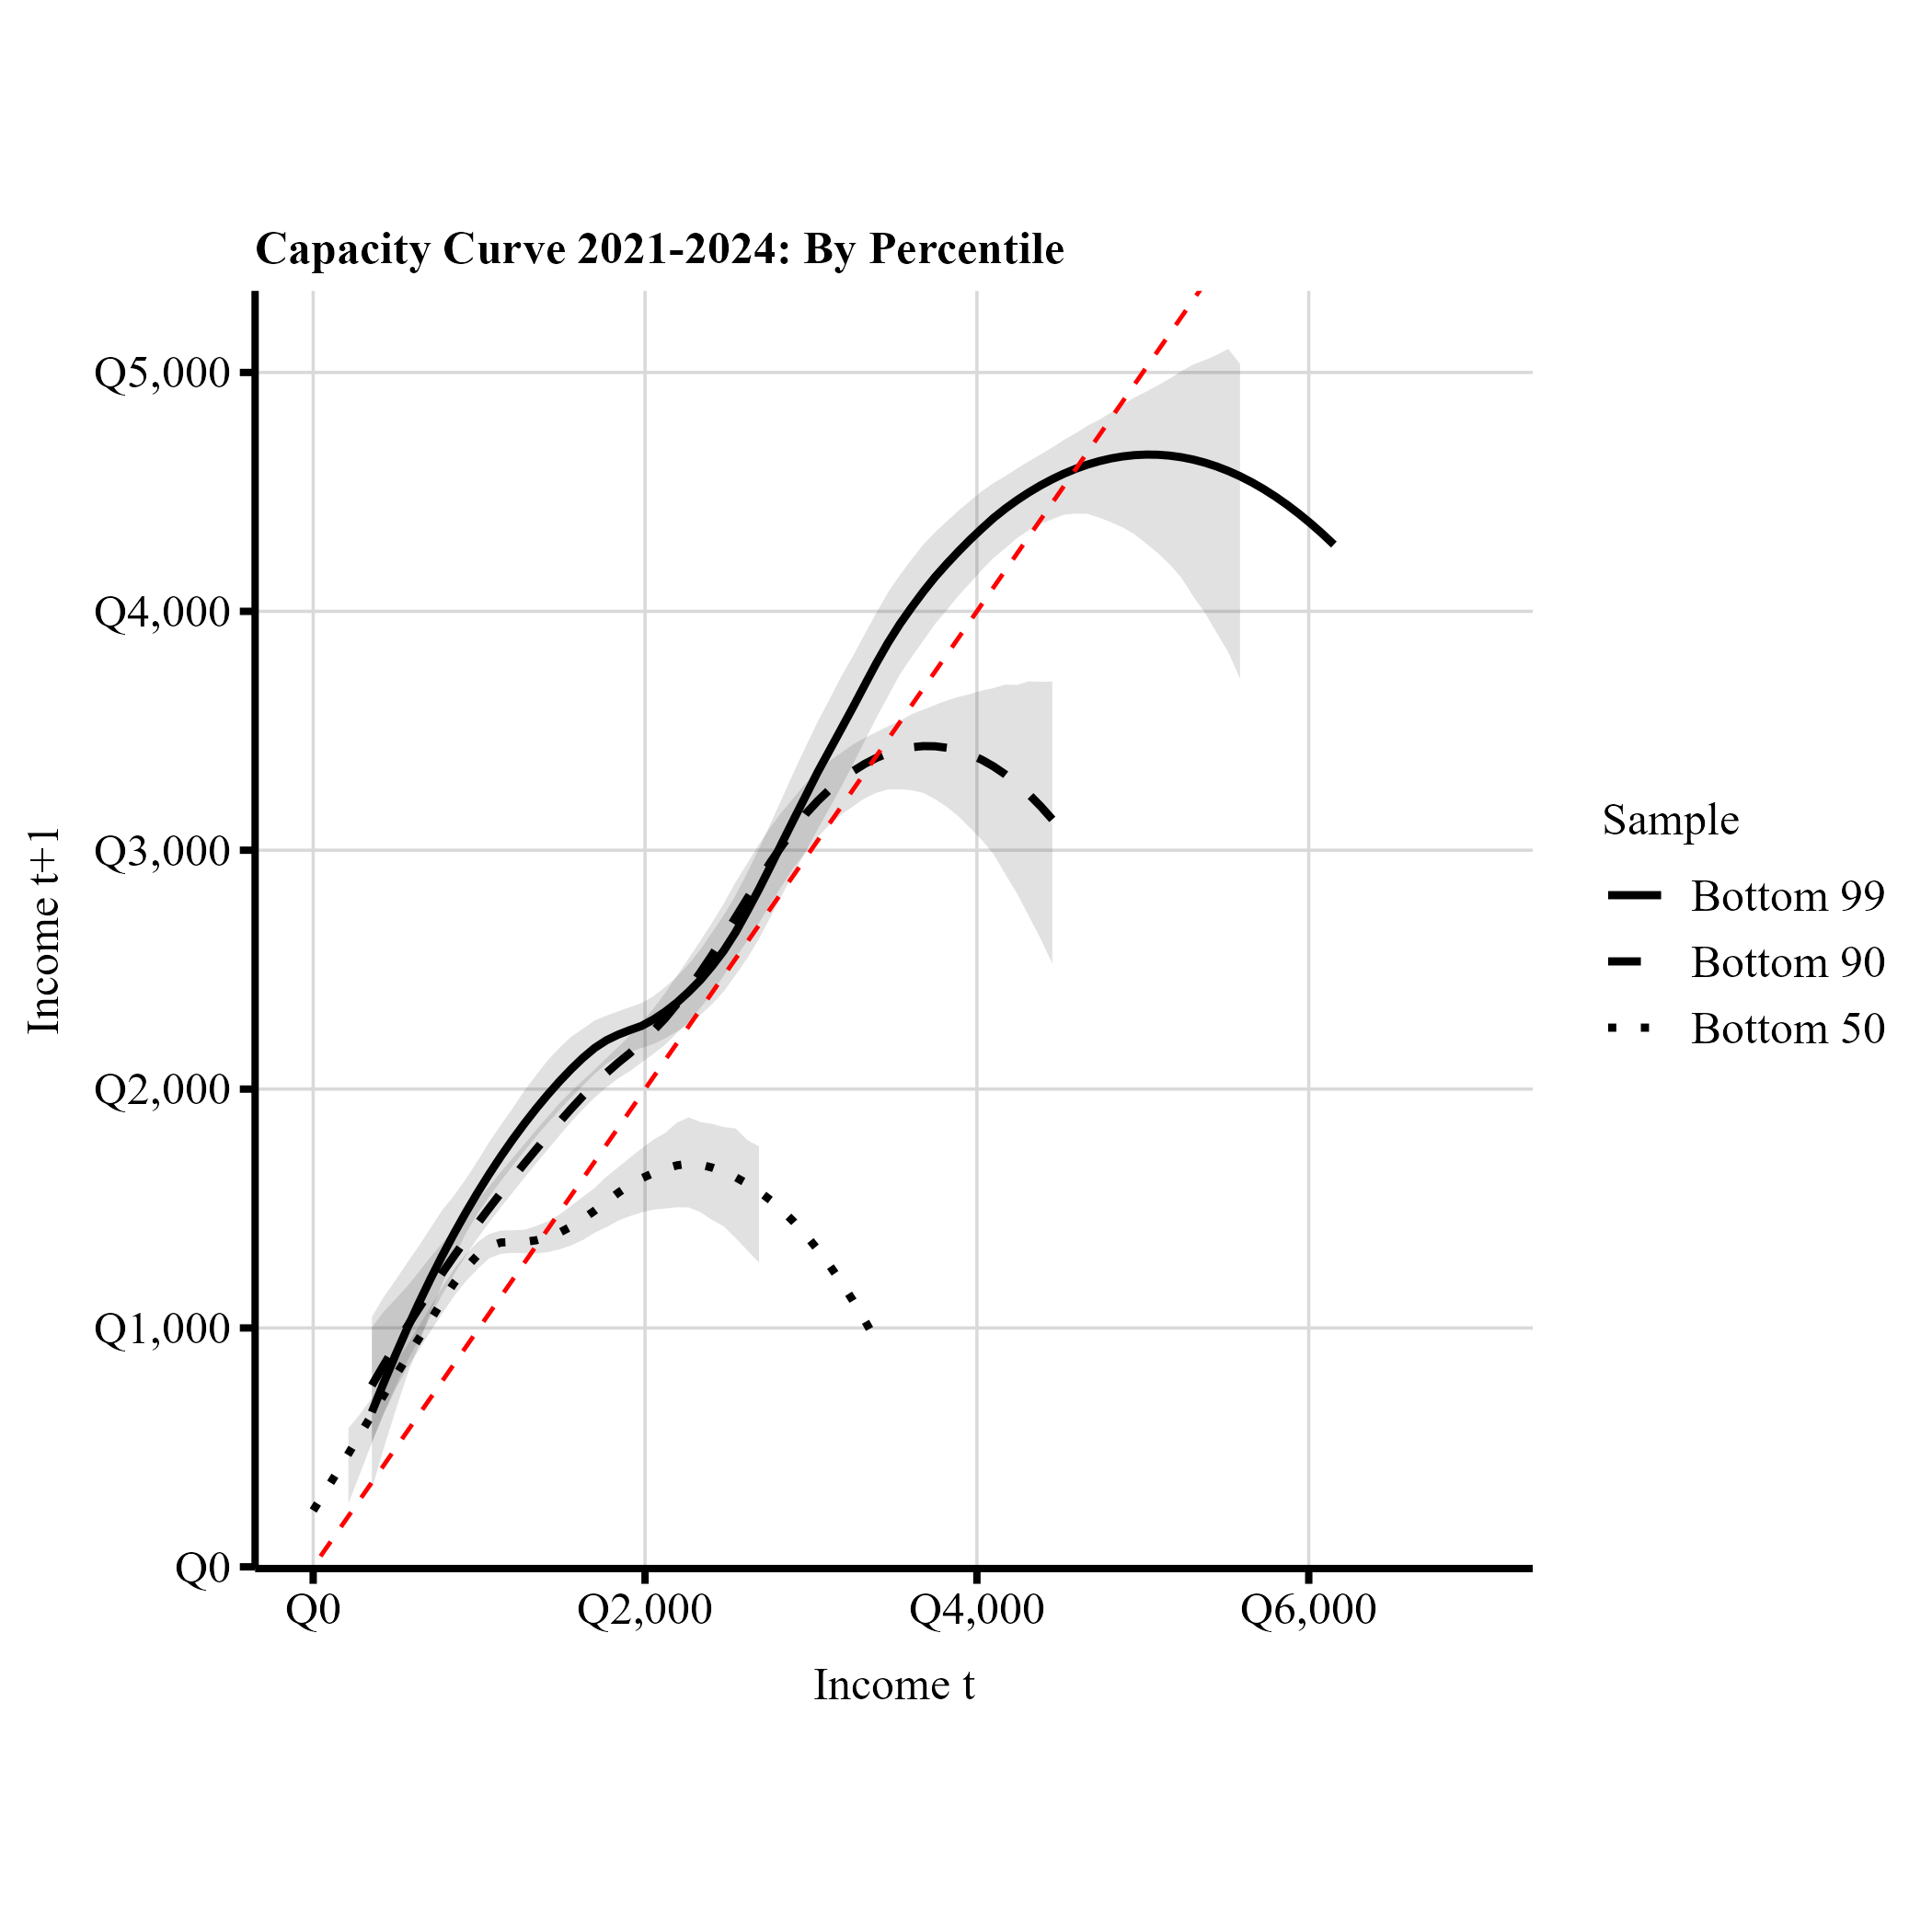
\includegraphics[trim={0.72bp 51.36bp 5.28bp 50.64bp},clip,width=0.90\linewidth,height=0.36\textheight,keepaspectratio]{figures/main-2021-2024-figure5.png}
\caption{Capacity curves: Income percentiles, 2021-2024.}
\label{fig:main-2021-2024-5}
\end{figure}


\clearpage

\section{Conclusion}
Poverty is a multidimensional problem with no magic solution. Over the last three decades, humanity has made substantial progress in identifying successful strategies to fight it and achieve significant reductions in the short and long run. However, studying the persistence of poverty across the population requires examining its evolution over time, not only aggregate trends. This presents important challenges, especially in the developing world, where access to high-quality longitudinal datasets is limited. Pseudo-panel analysis therefore offers a relevant alternative for studying poverty persistence and identifying poverty traps across countries.

Using data from Guatemala to test this approach, we provide empirical estimates of the capacity curve for the employed working-age population. The estimates indicate that the capacity curve for 2016--2019 was largely linear and close to the 45-degree line. However, after the pandemic shock, the shape of the curve changed substantially, suggesting that a second, lower steady state merits consideration, although its existence remains unresolved. A plausible interpretation of the patterns across population subgroups is that the post-pandemic changes could reflect a deprivation poverty trap rather than a convergence trap. This perspective draws on the heterogeneous changes in income dynamics observed across groups defined by gender, geographic area, and income level; it leaves the existence and type of trap open and does not attribute its emergence causally to the pandemic. The only variable supporting initial differences in conditions between population groups is indigenous status. Although these differences may exist, the deprivation aspect of the trap could dominate under this reading.

Nevertheless, even if there was some degree of mobility before the COVID-19 crisis, the upper apparent convergence point was not necessarily high, lying near Q6,000 (approximately \$775), which is barely enough to cover essential goods and a dignified standard of living. Taken together, these findings point to two policy directions. First, they support the need to find policies that could shift the capacity curve upward and raise the original steady state, so that Guatemalans could actually experience income mobility. Second, it is important to pay attention to lower-income individuals, who may face even stronger limitations on their economic prosperity than before the pandemic, potentially leaving them at subsistence levels. Policymakers should aim to ensure that the change in the shape of the capacity curve that appears to be associated with the pandemic is temporary and fades over time.

\section{AI-Use Disclosure}

The authors used agentic AI tools, including Claude Code and Codex, to support code debugging and to review parts of the statistical inference procedure, including the construction of confidence bands, bootstrap implementation, and cross-validation for bandwidth selection. These tools were also used to identify spelling and grammatical errors, improve readability, and proofread the manuscript before submission. All methodological decisions, code, results, and interpretations were reviewed and validated by the authors.

\section{Funding}

This research received no external funding. None of the authors received compensation for conducting this study, and all work related to the project was completed during the authors' personal time.

\section{Author Contributions}

\textbf{Fernando Sáenz:} Conceptualization of the main research question and empirical approach; development of the non-parametric estimation strategy; initial development of the data cleaning, merging, and analysis code in R for the 2016--2019 period; robustness analysis; methodology; results; and manuscript drafting.

\textbf{Alejandro Milián:} Creation and maintenance of the collaborative GitHub repository; development of the data cleaning code for the 2021--2024 period; and restructuring and organization of the current codebase.

\textbf{Javier Velásquez:} Literature review; identification and review of relevant international and Guatemalan studies; and drafting of the literature review section.

\clearpage
\printbibliography

\clearpage
\appendix
\setcounter{figure}{0}
\setcounter{table}{0}
\renewcommand{\thefigure}{A\arabic{figure}}
\renewcommand{\thetable}{A\arabic{table}}
\section{Supplementary figures}
\label{app:figures}

\begin{figure}[!htbp]
\singlespacing
\centering
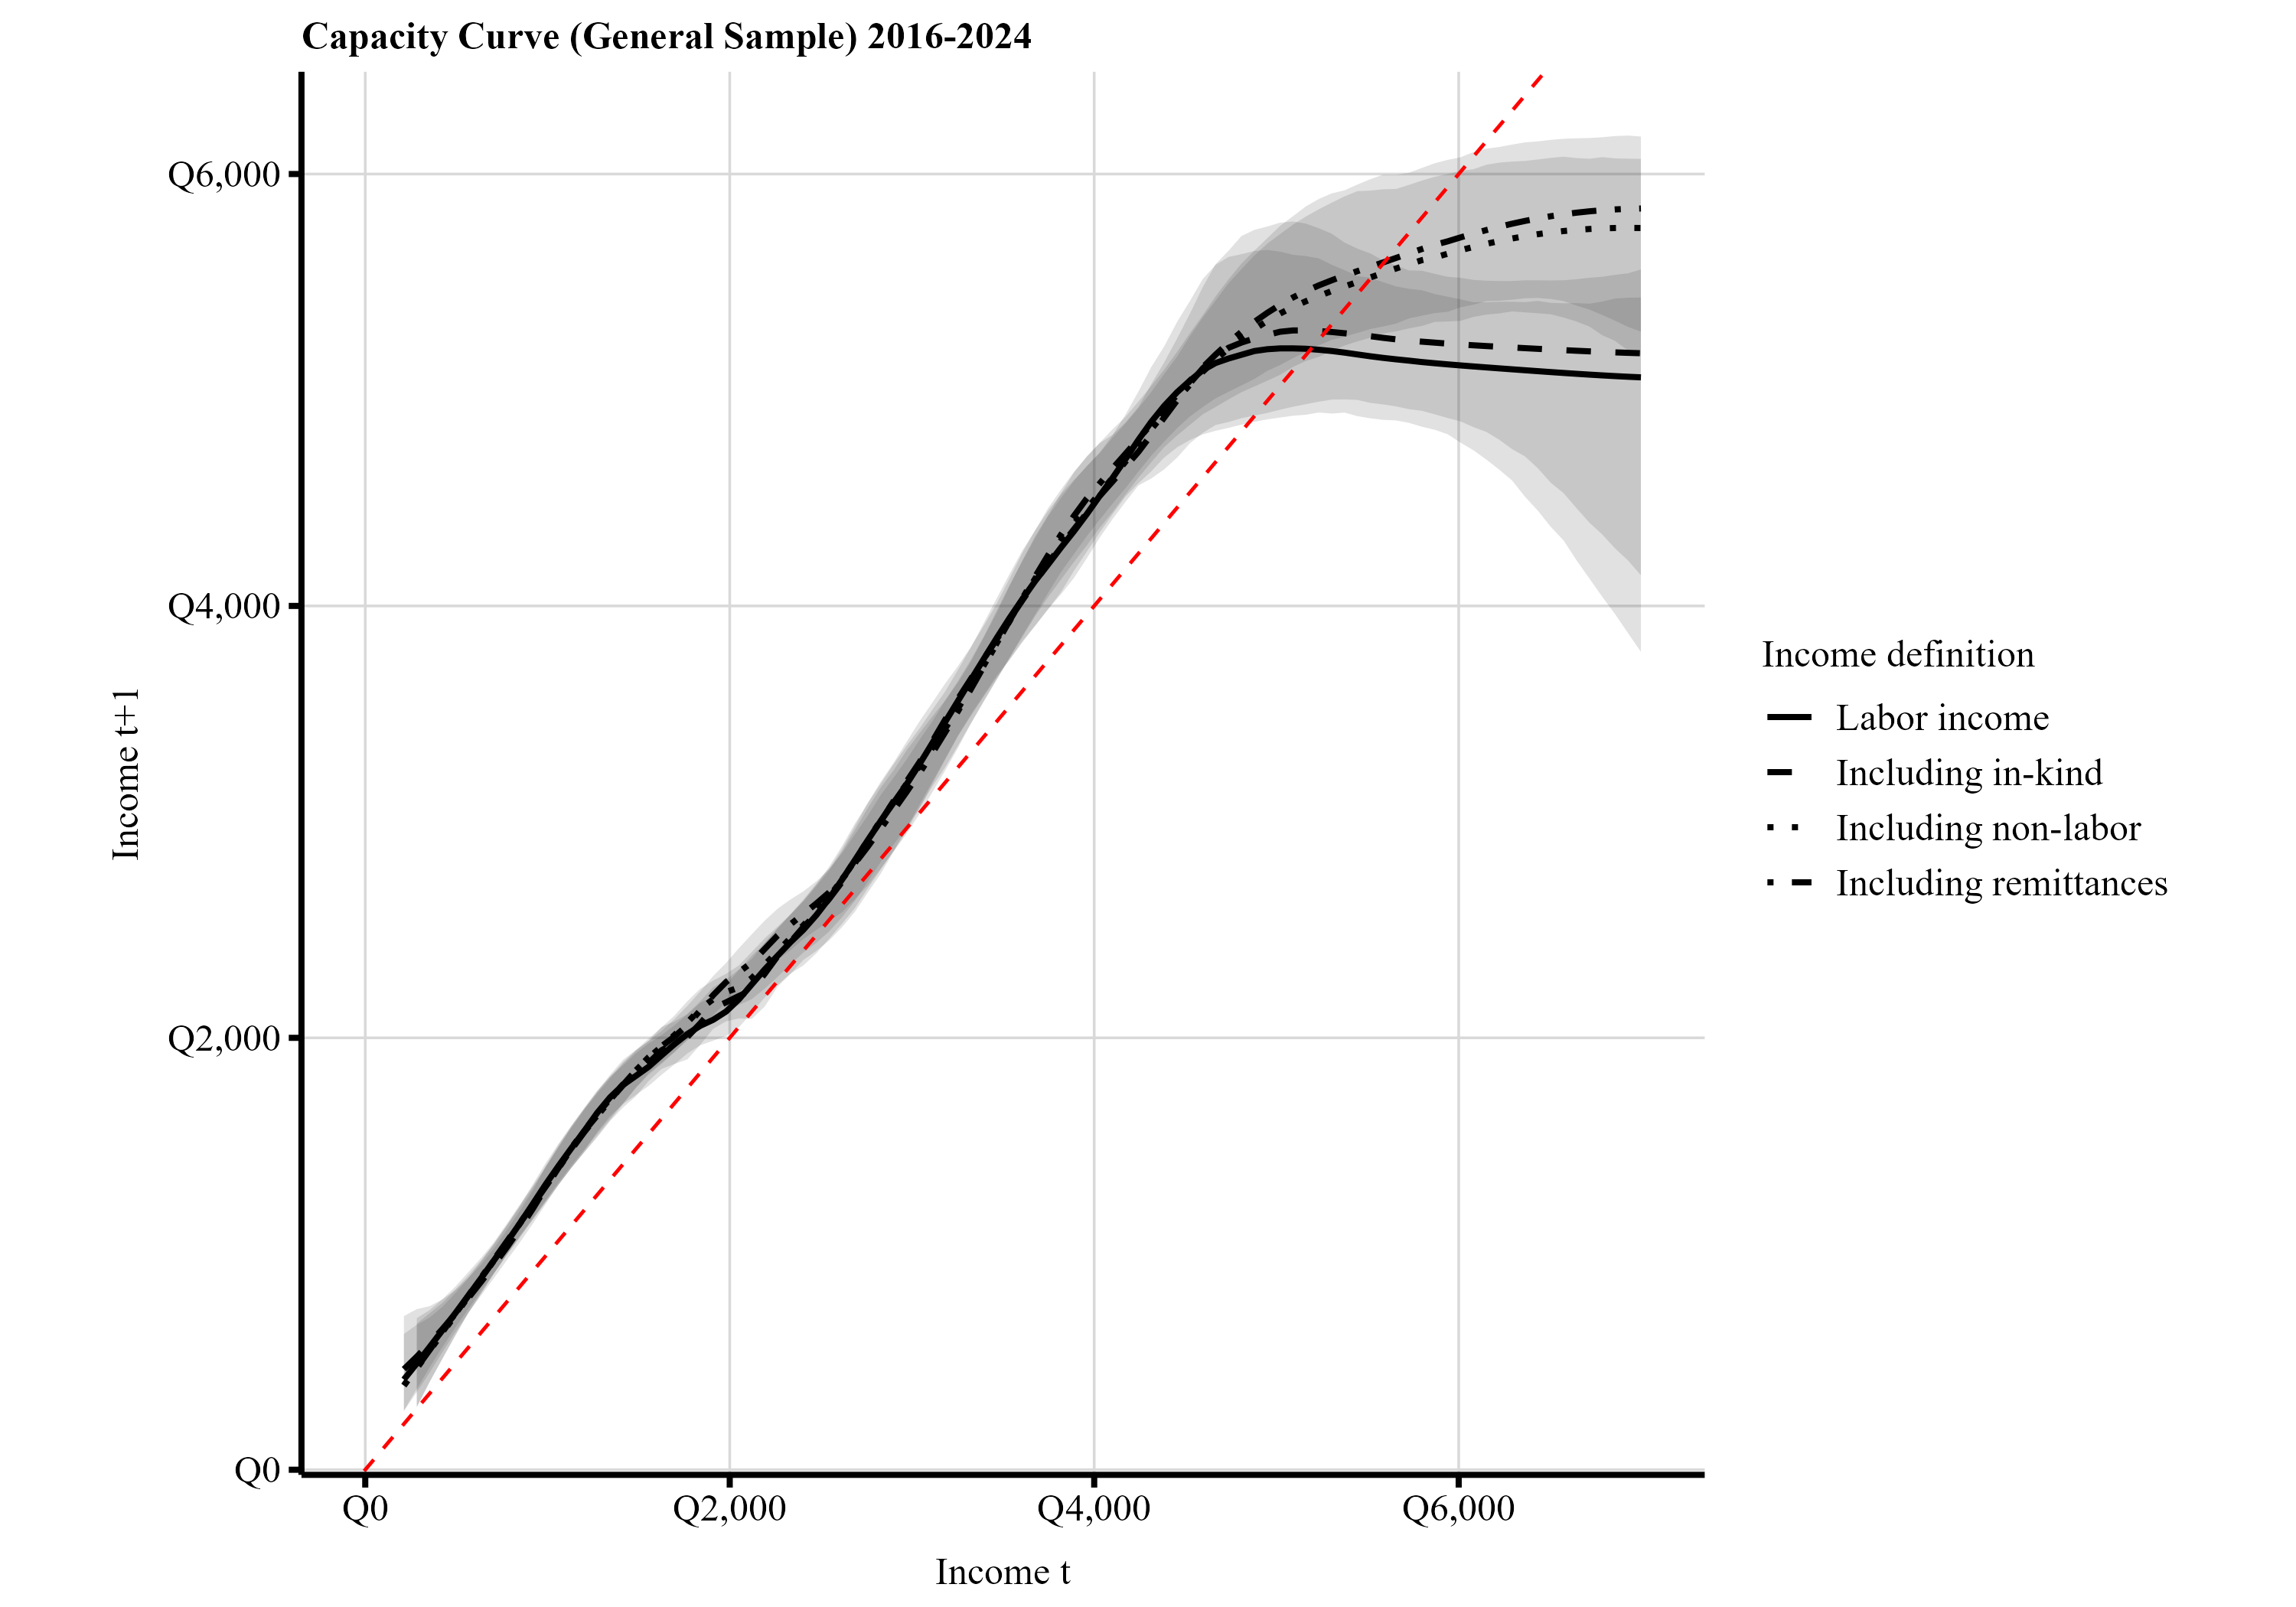
\includegraphics[trim={27.60bp 0.00bp 33.12bp 0.00bp},clip,width=0.90\linewidth,height=0.36\textheight,keepaspectratio]{figures/pooled-figure1.png}
\caption{Capacity curves: General sample, 2016-2024.}
\label{fig:pooled-1}
\end{figure}

\begin{figure}[!htbp]
\singlespacing
\centering
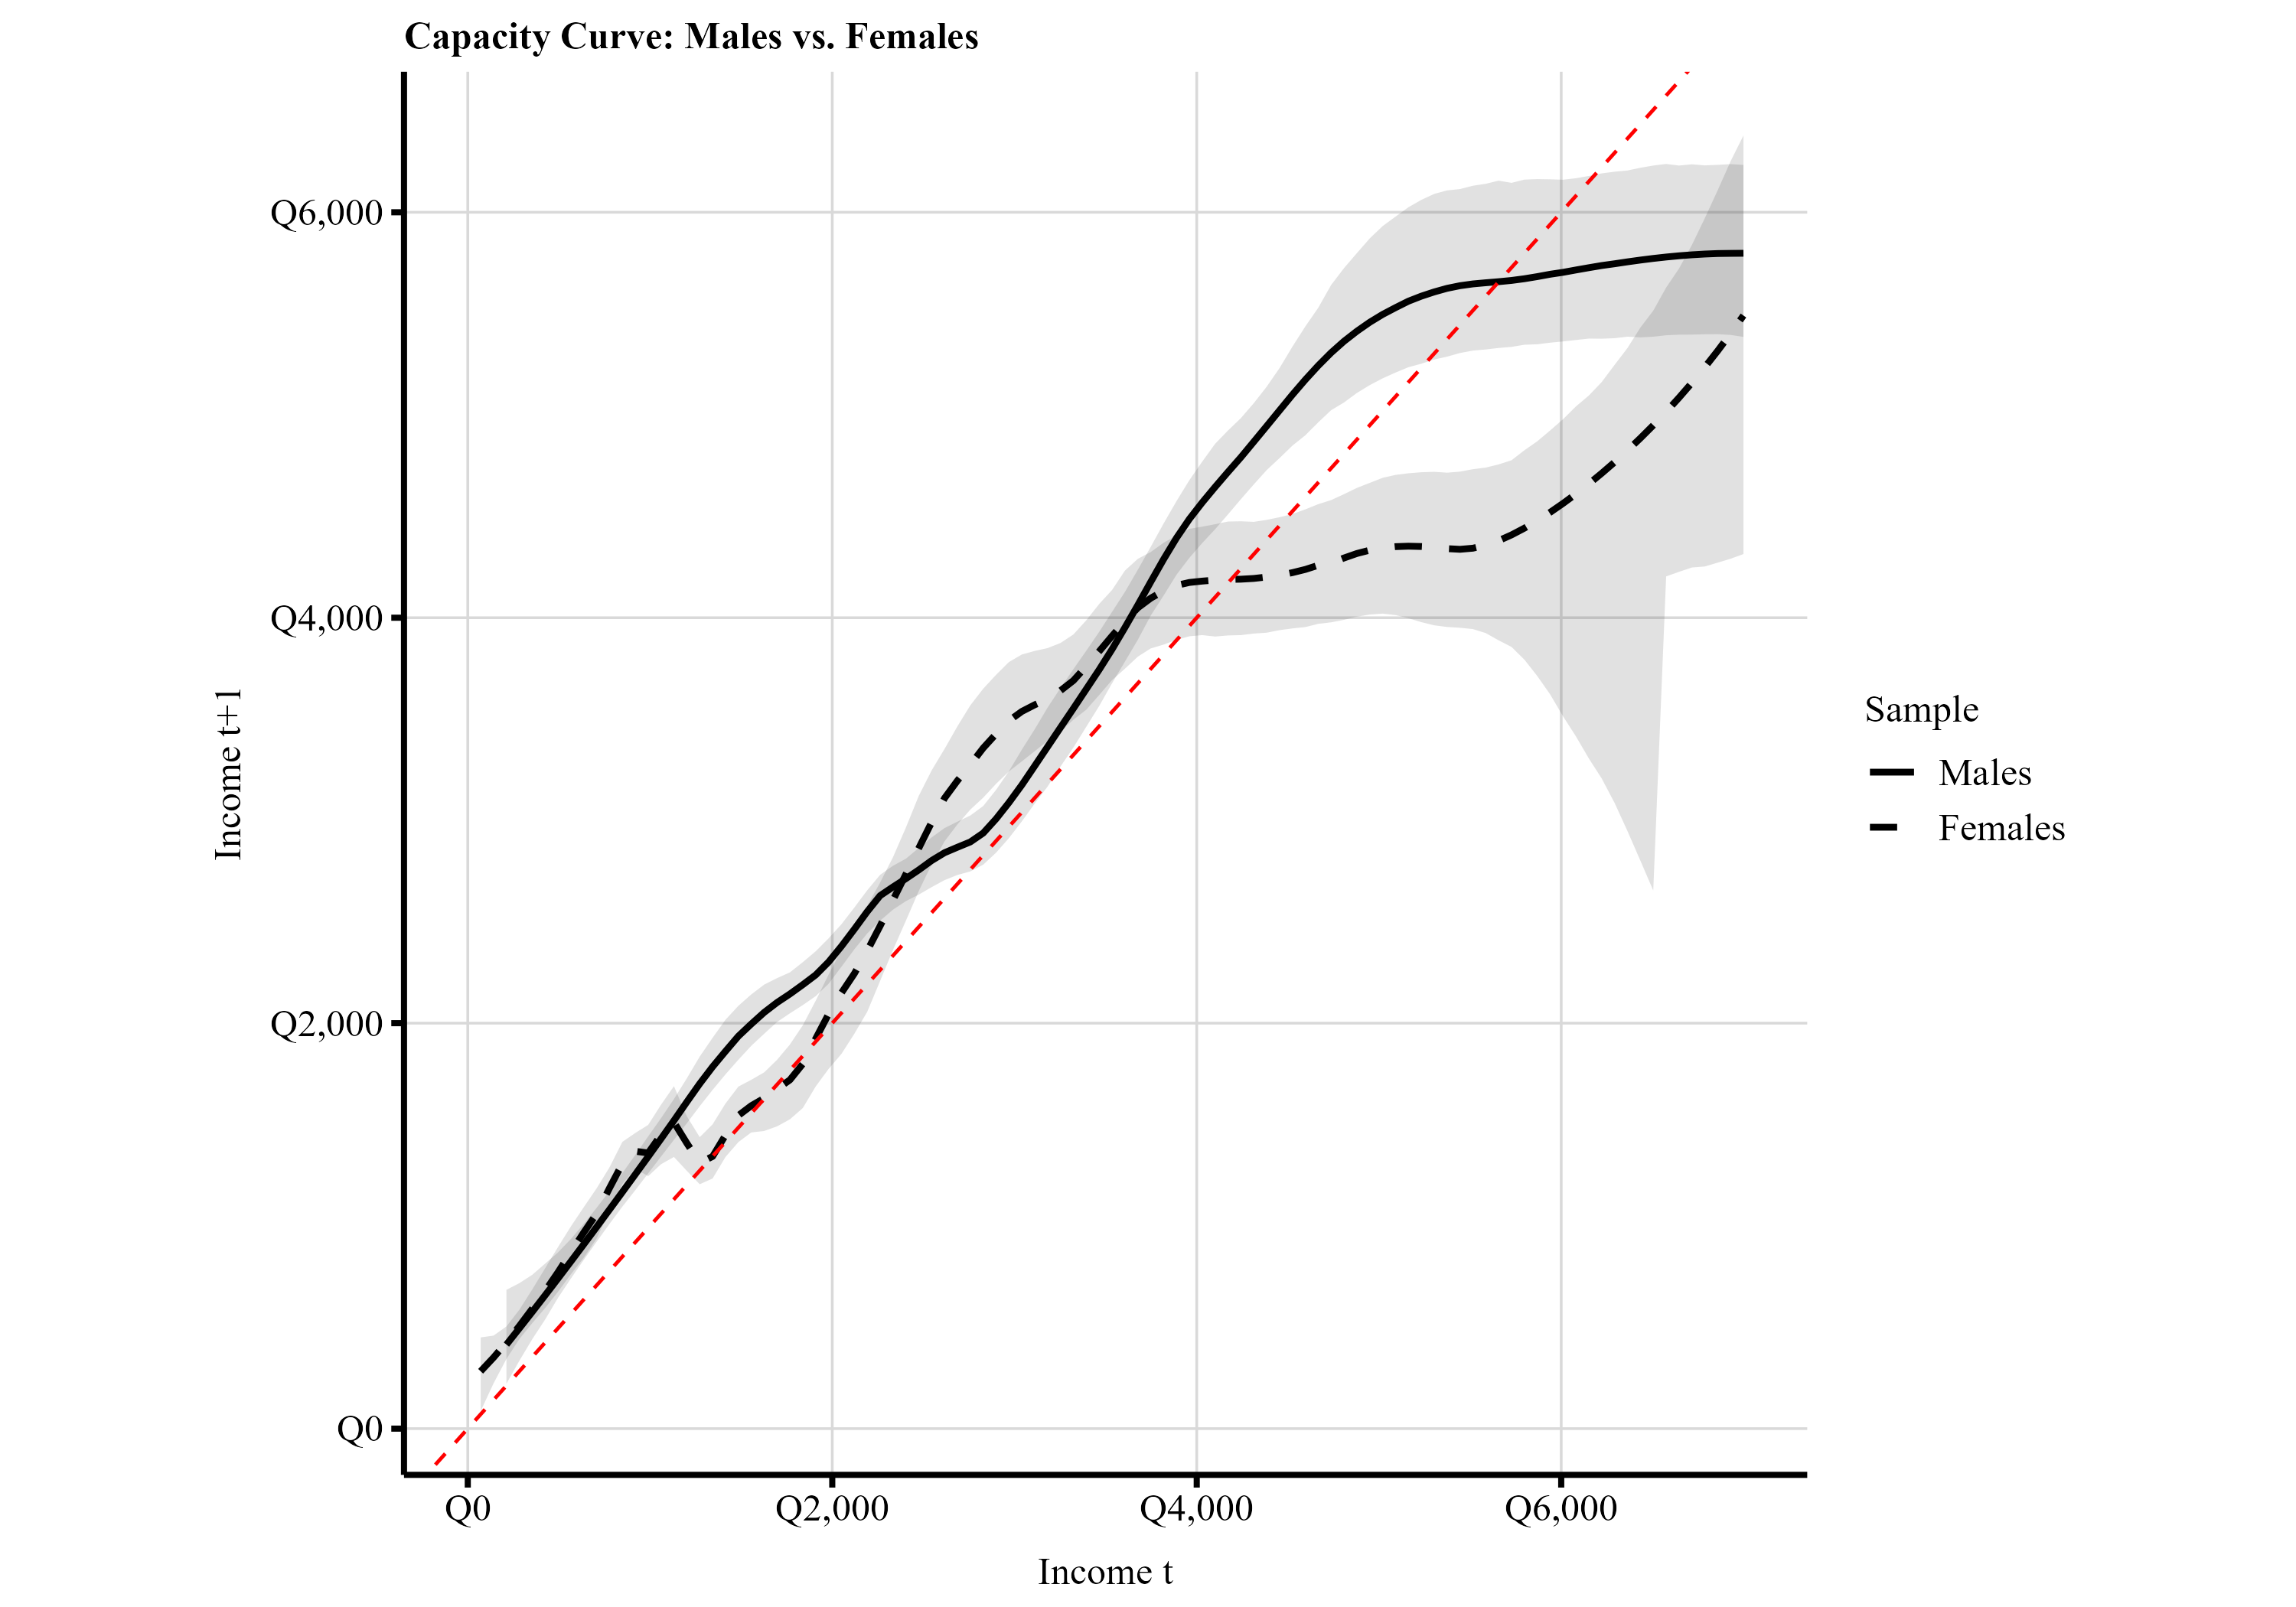
\includegraphics[trim={62.16bp 0.00bp 75.36bp 0.00bp},clip,width=0.90\linewidth,height=0.36\textheight,keepaspectratio]{figures/pooled-figure2.png}
\caption{Capacity curves: Males and females, 2016-2024.}
\label{fig:pooled-2}
\end{figure}

\begin{figure}[!htbp]
\singlespacing
\centering
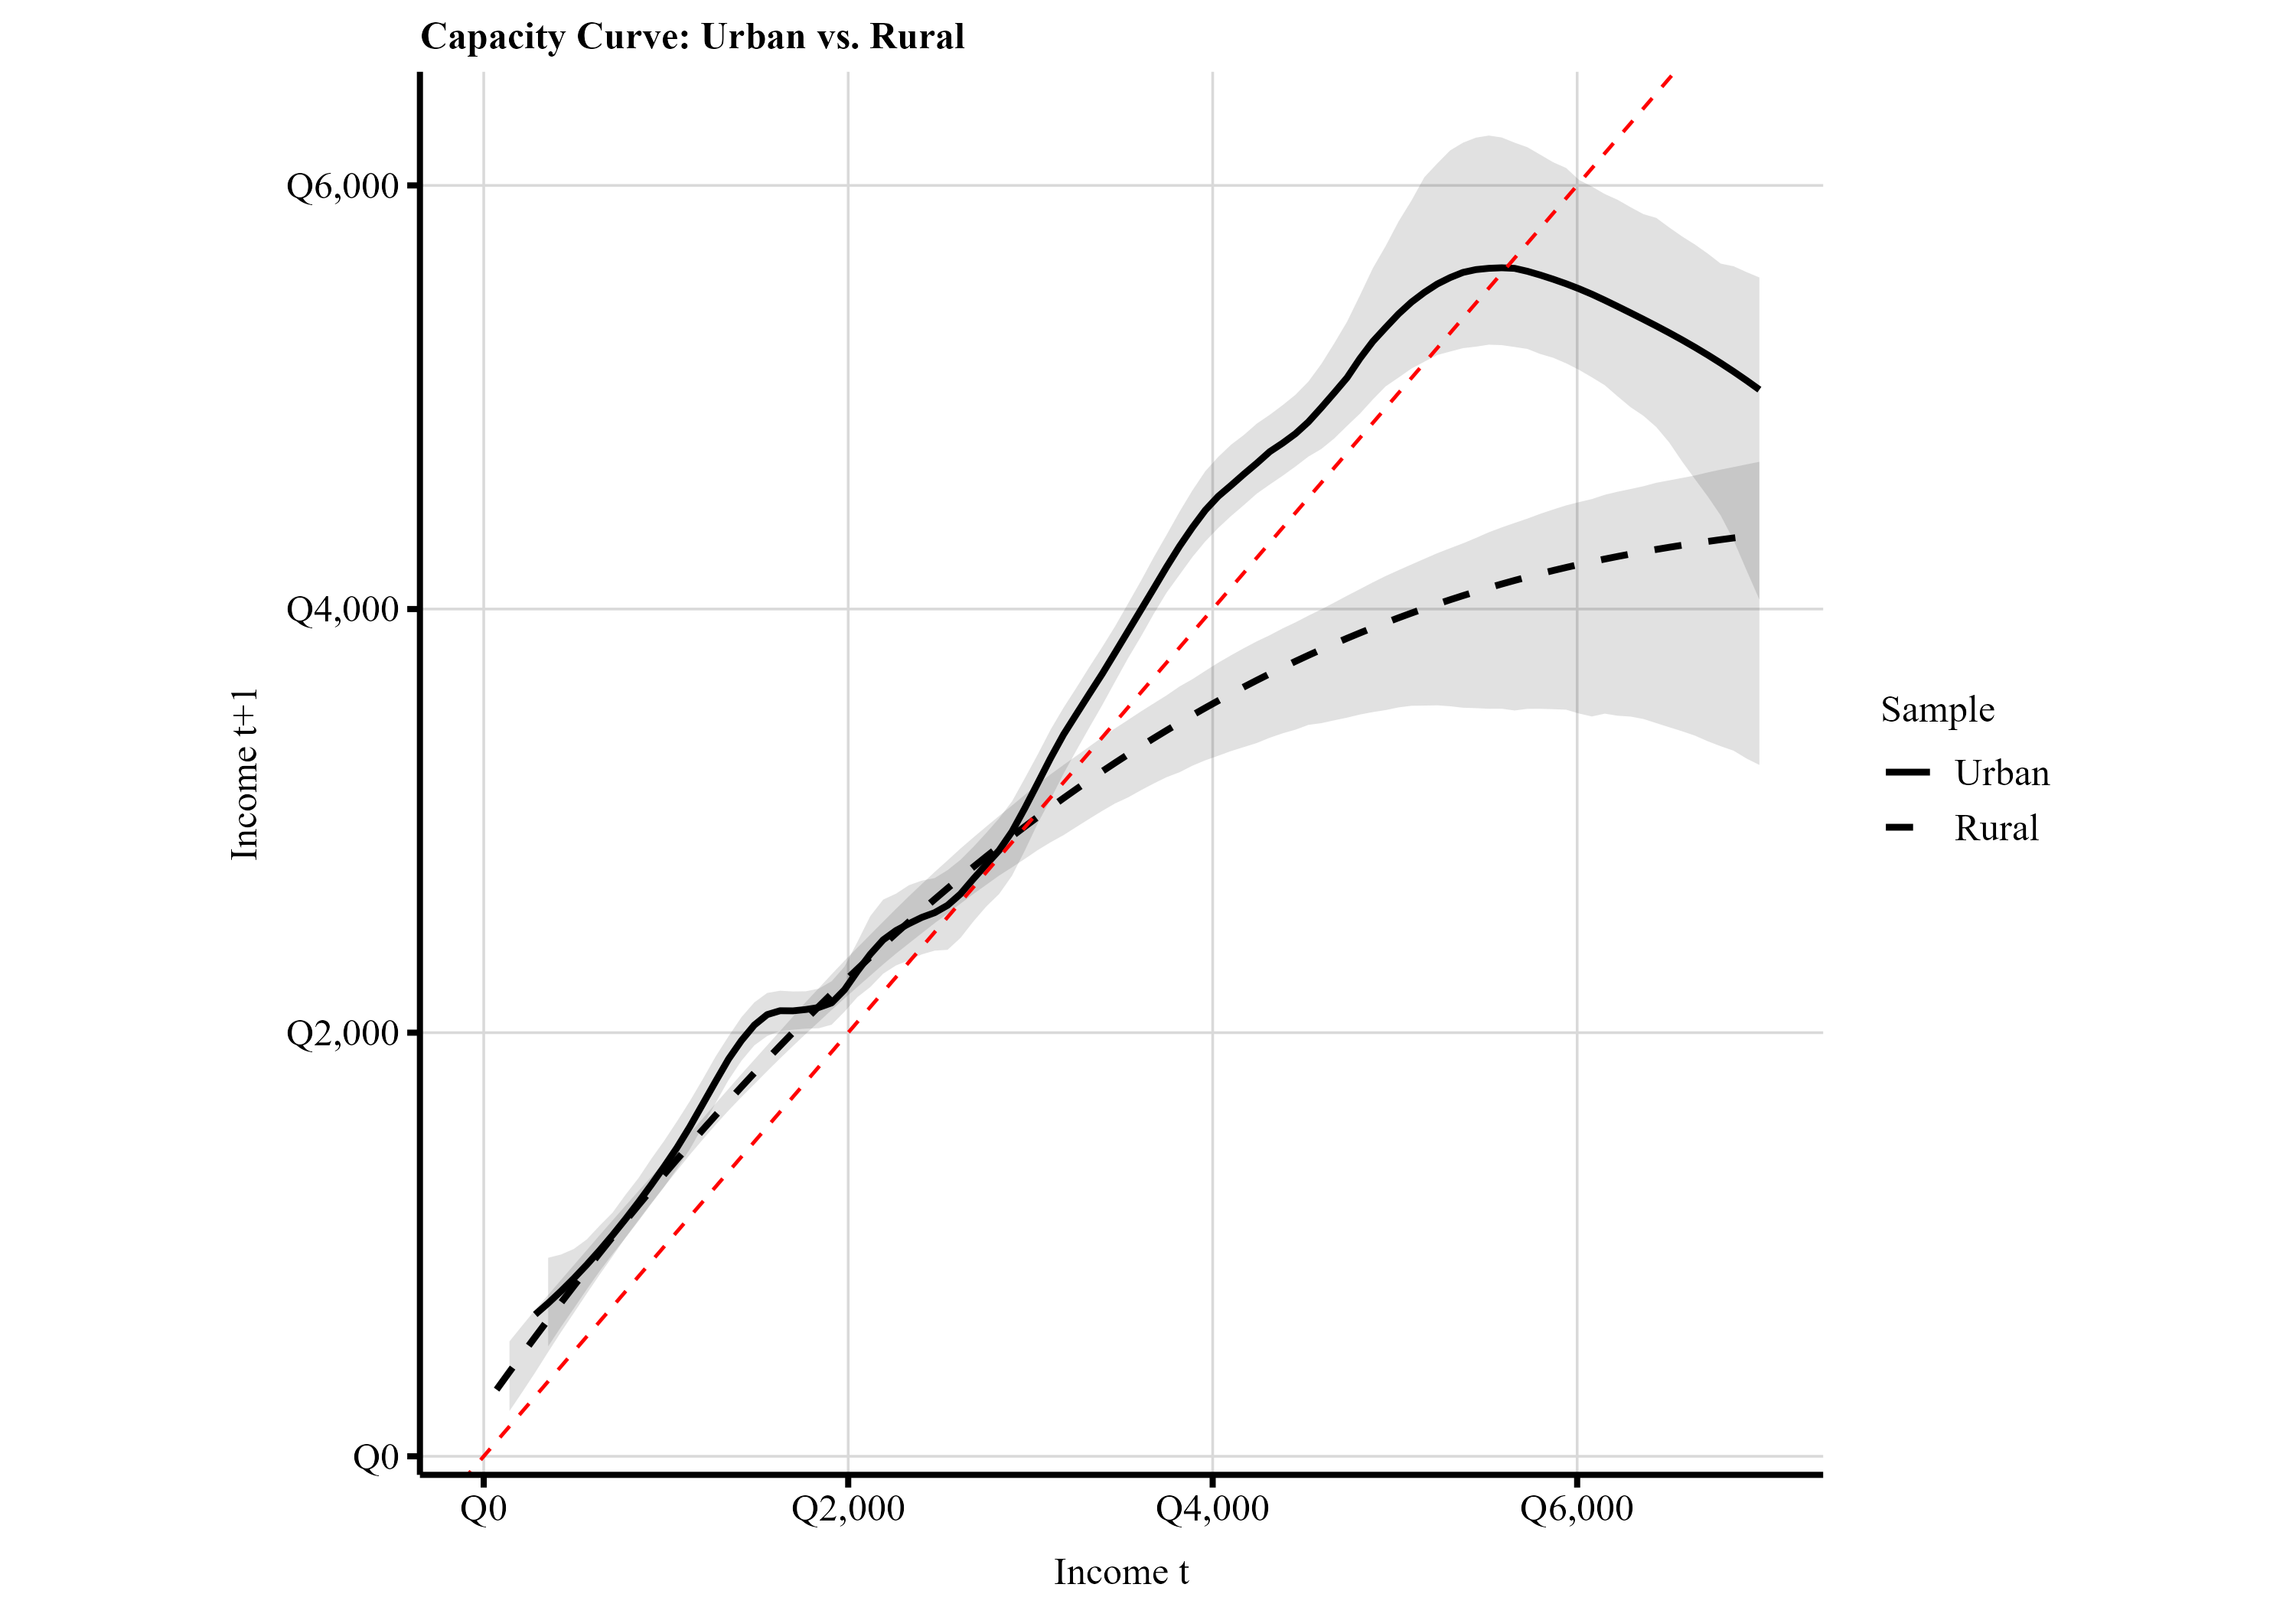
\includegraphics[trim={66.00bp 0.00bp 67.68bp 0.00bp},clip,width=0.90\linewidth,height=0.36\textheight,keepaspectratio]{figures/pooled-figure3.png}
\caption{Capacity curves: Urban and rural populations, 2016-2024.}
\label{fig:pooled-3}
\end{figure}

\begin{figure}[!htbp]
\singlespacing
\centering
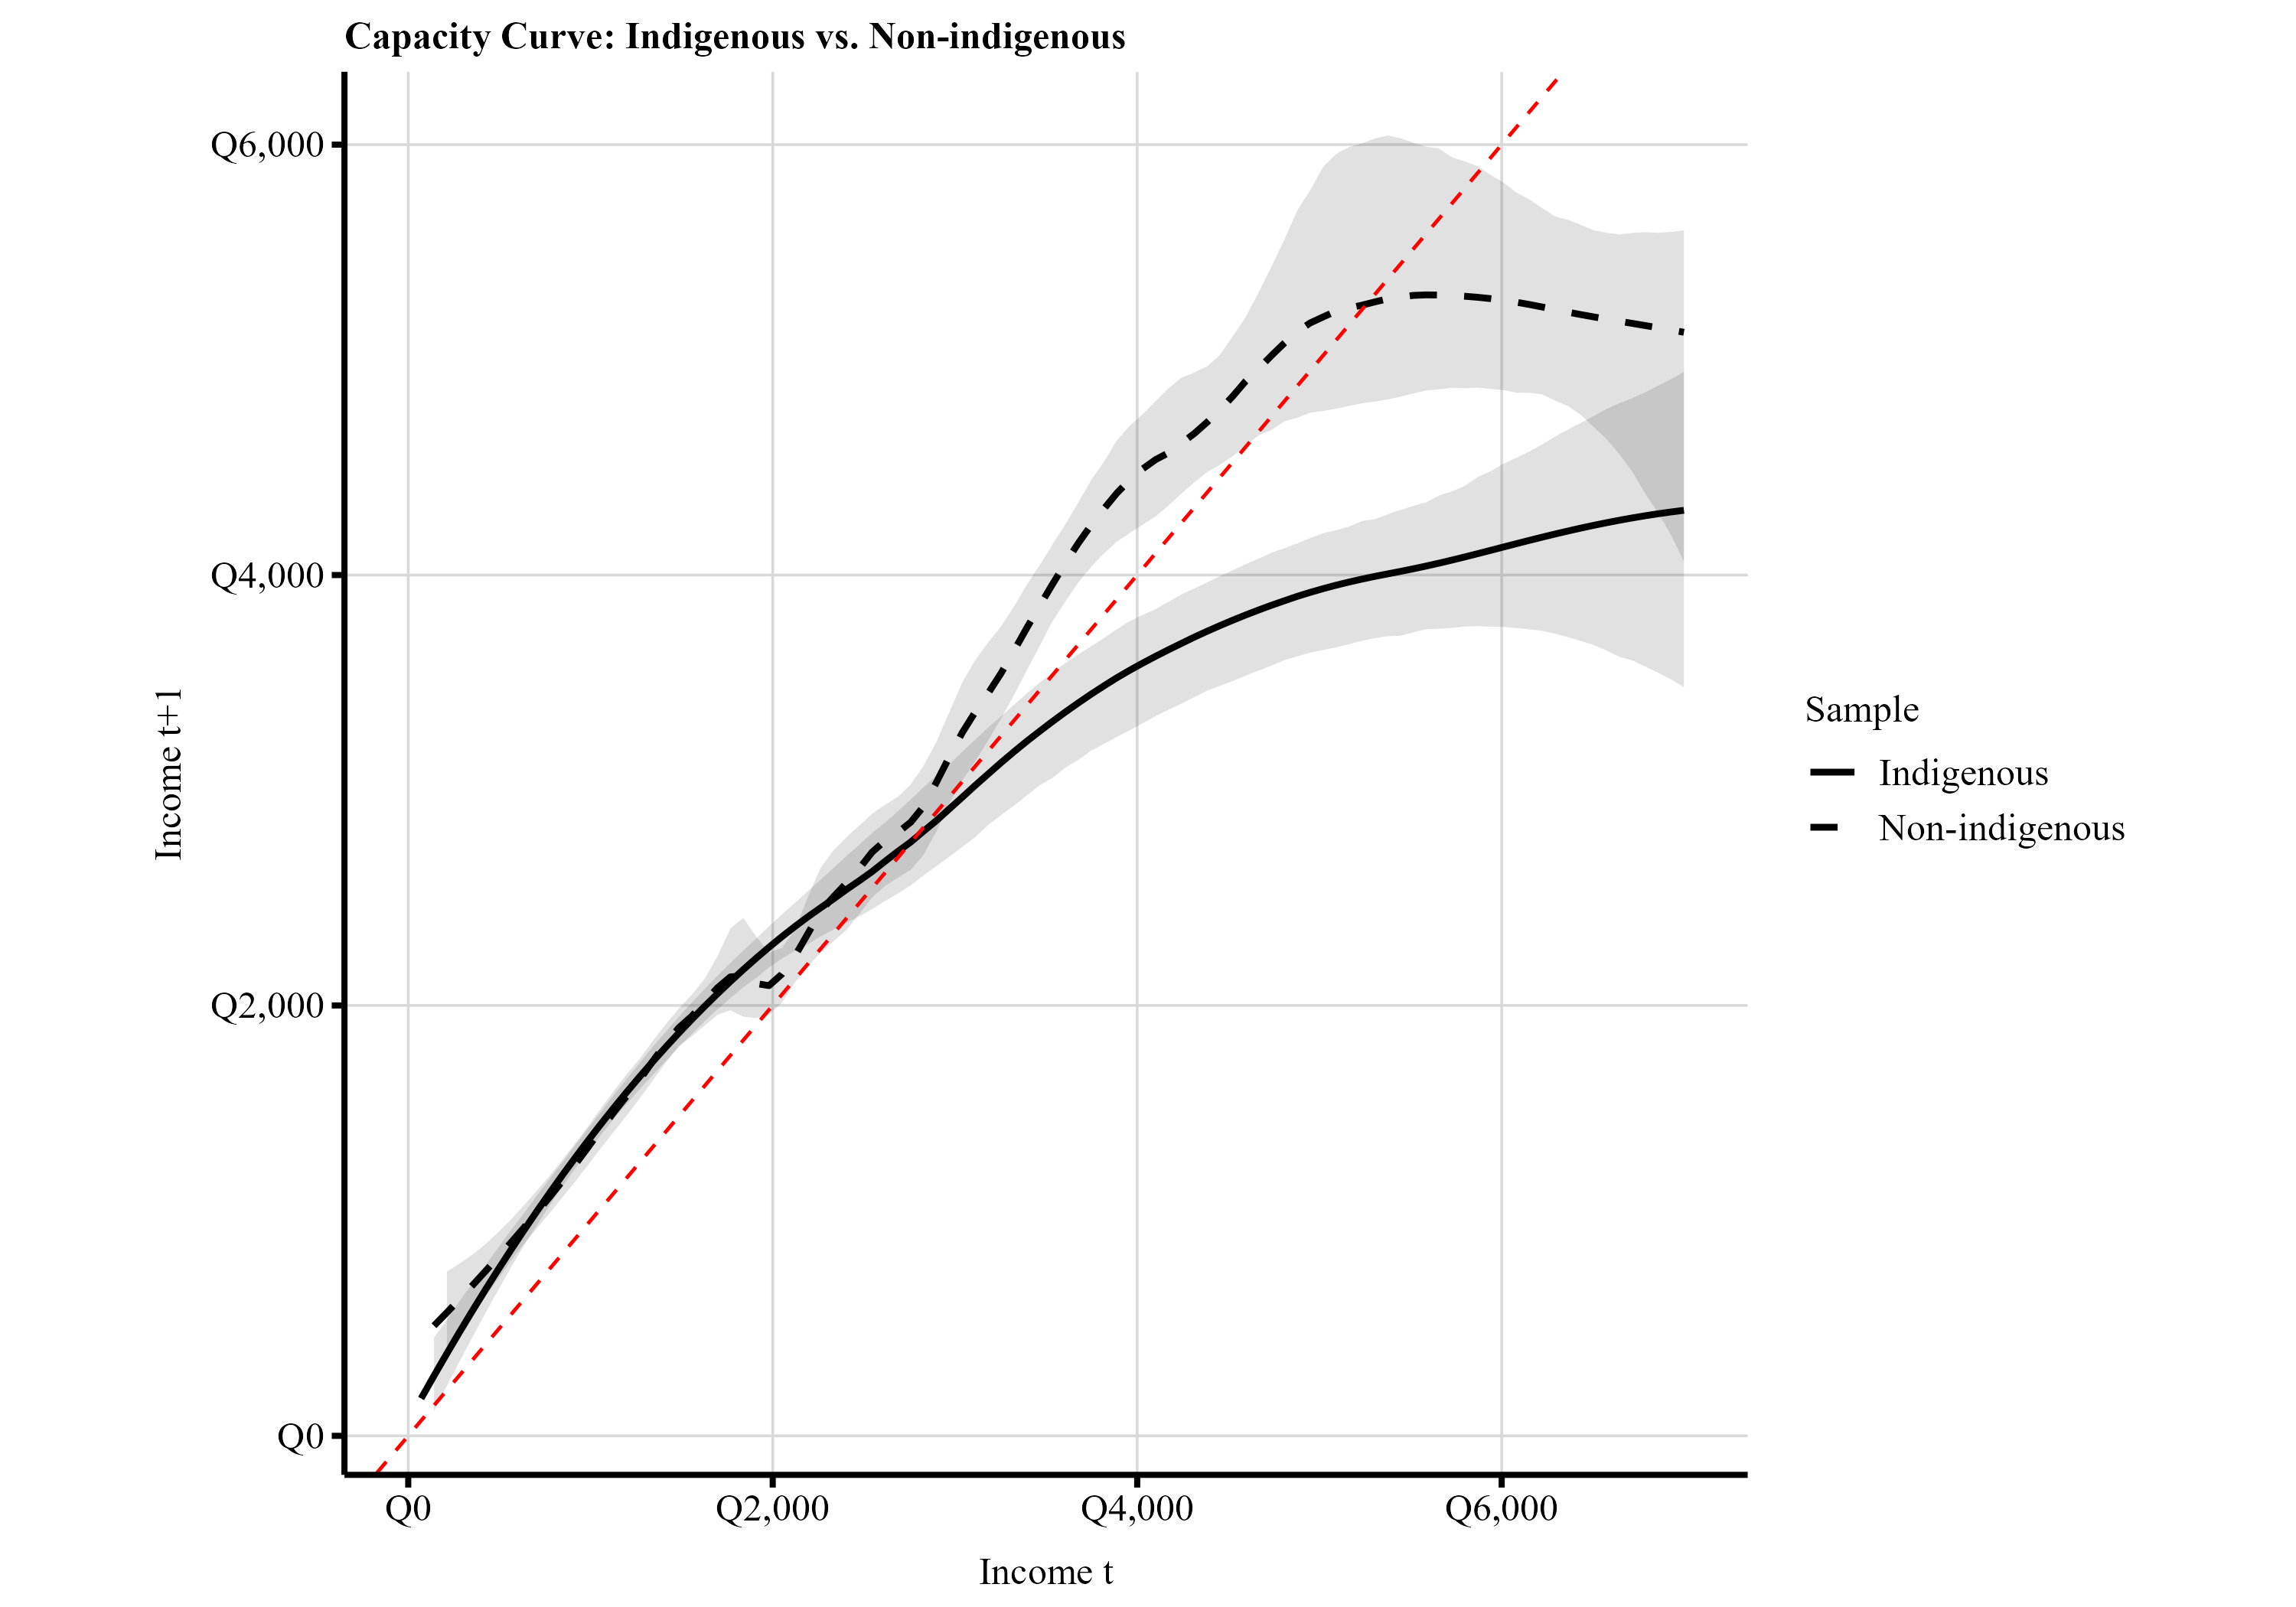
\includegraphics[trim={42.96bp 0.00bp 44.64bp 0.00bp},clip,width=0.90\linewidth,height=0.36\textheight,keepaspectratio]{figures/pooled-figure4.png}
\caption{Capacity curves: Indigenous and non-indigenous populations, 2016-2024.}
\label{fig:pooled-4}
\end{figure}

\begin{figure}[!htbp]
\singlespacing
\centering
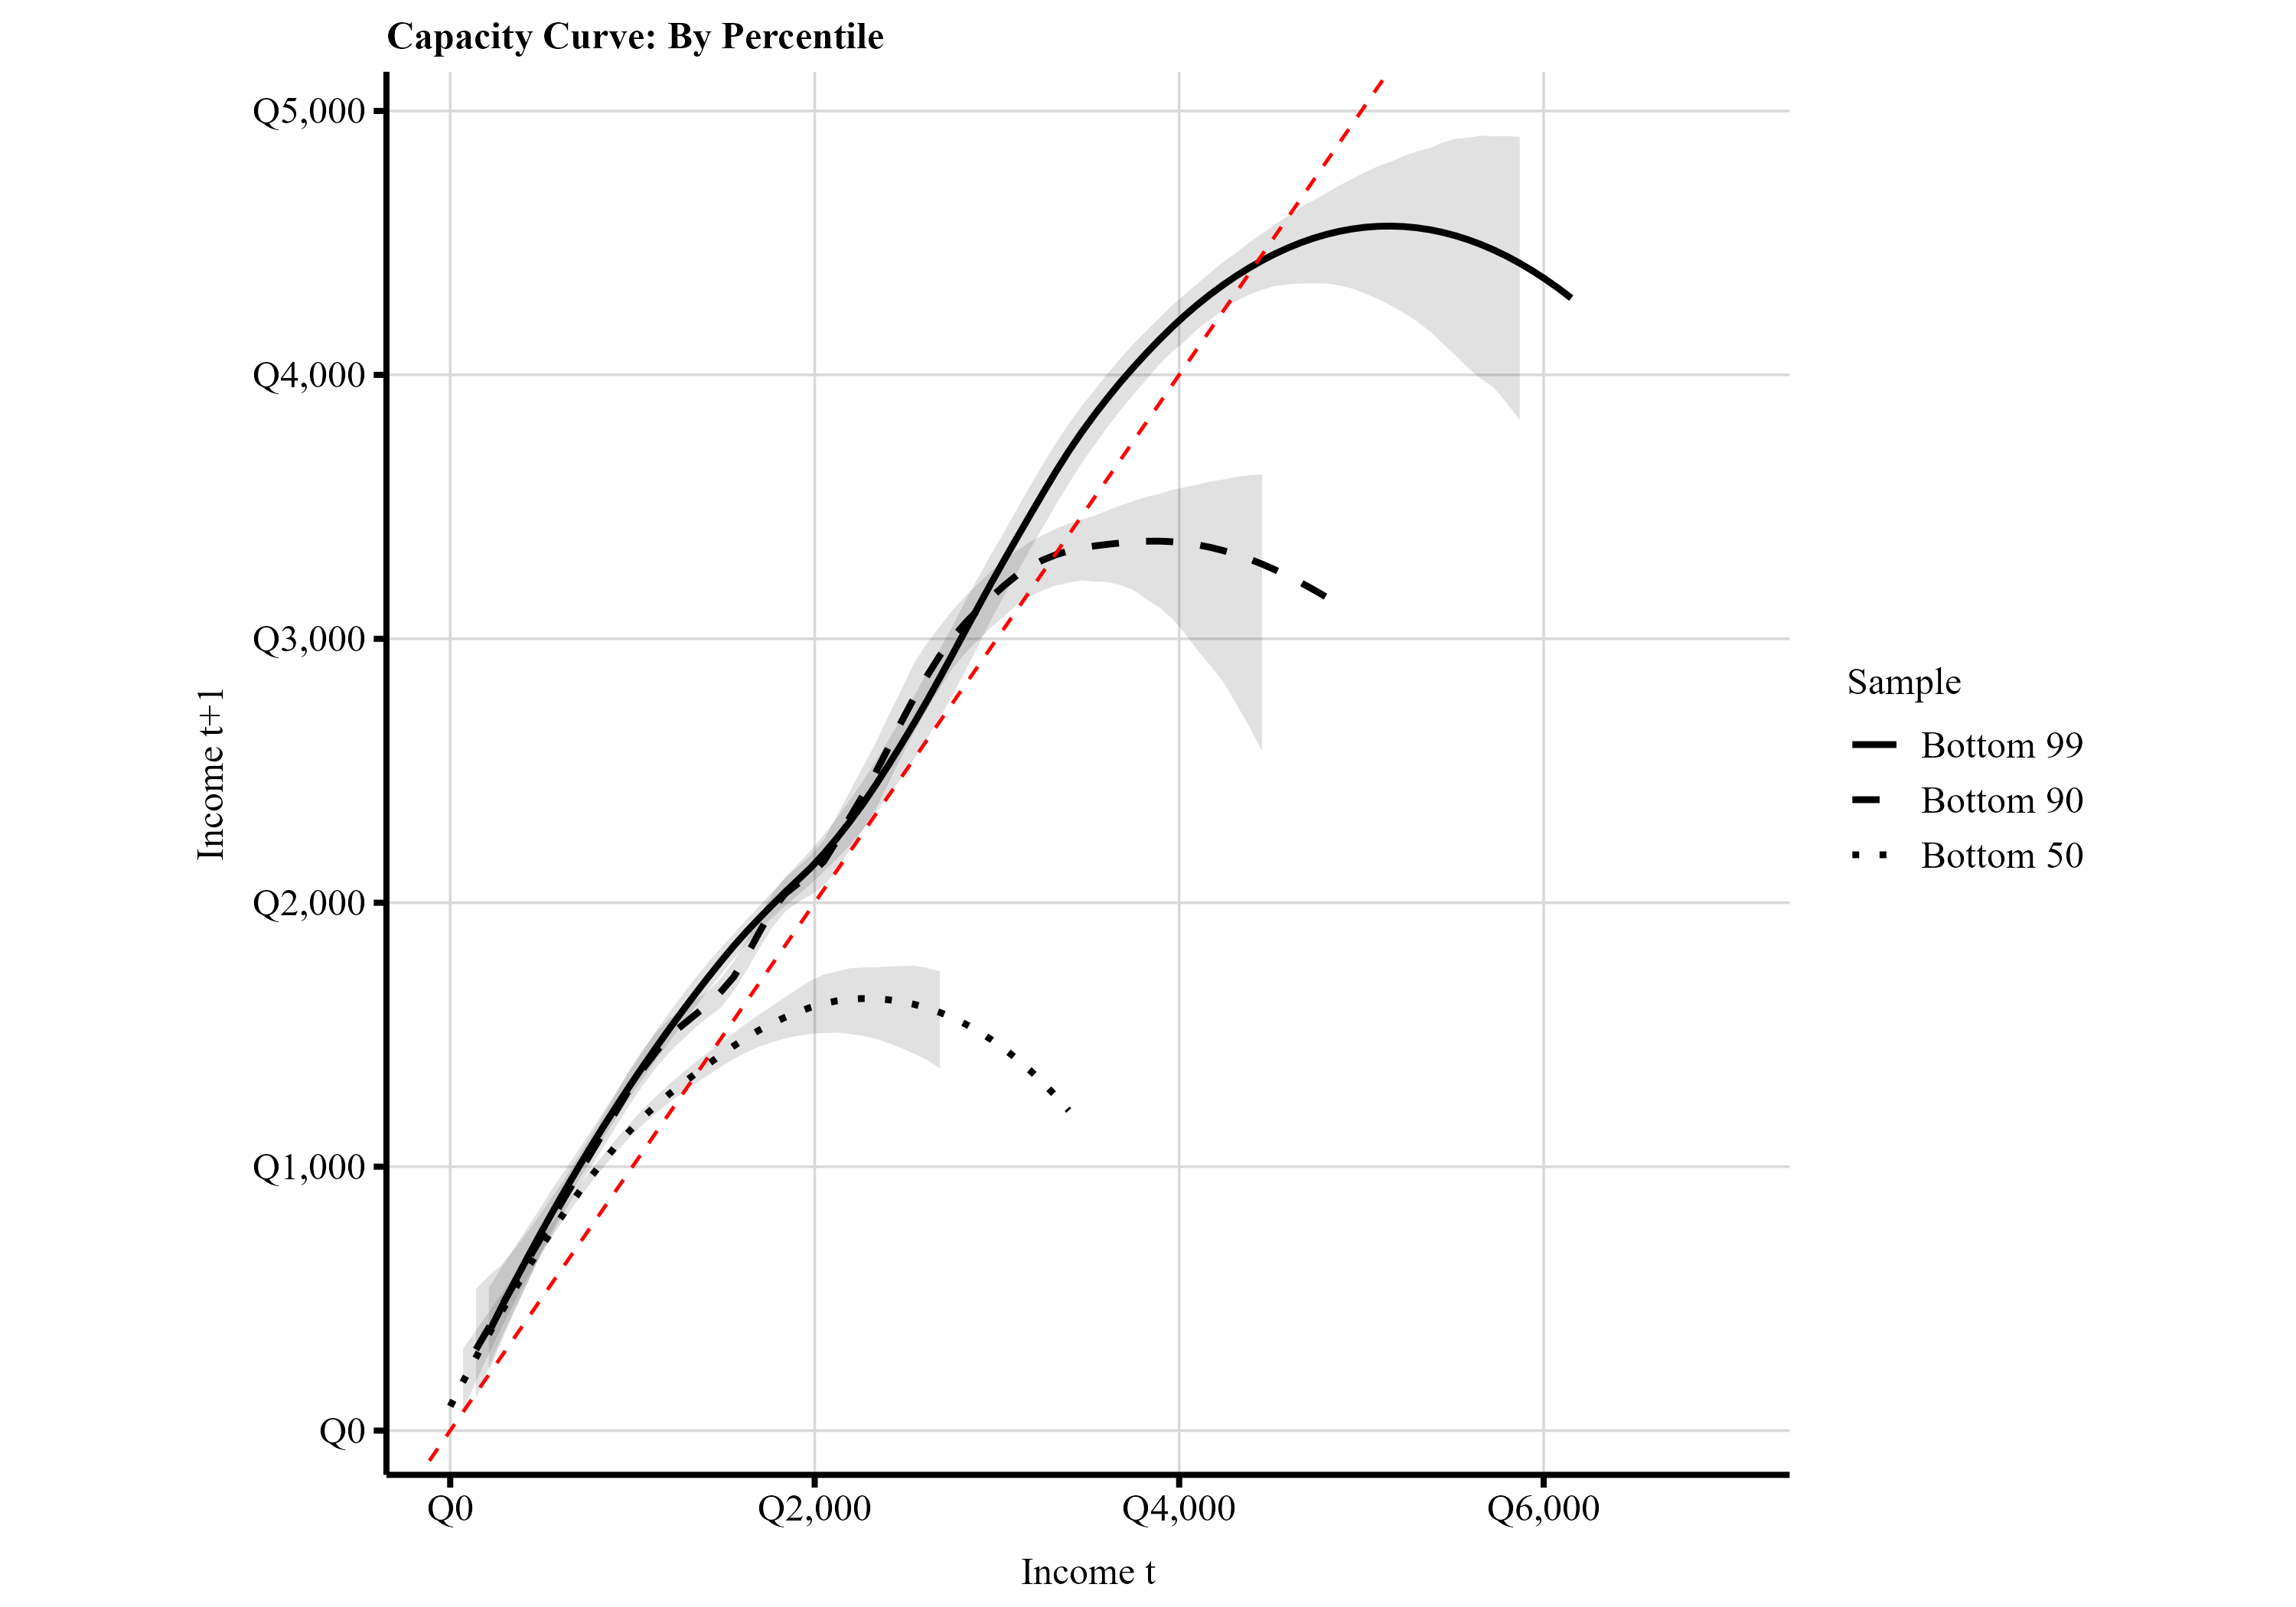
\includegraphics[trim={54.48bp 0.00bp 56.16bp 0.00bp},clip,width=0.90\linewidth,height=0.36\textheight,keepaspectratio]{figures/pooled-figure5.png}
\caption{Capacity curves: Income percentiles, 2016-2024.}
\label{fig:pooled-5}
\end{figure}

\begin{figure}[!htbp]
\singlespacing
\centering
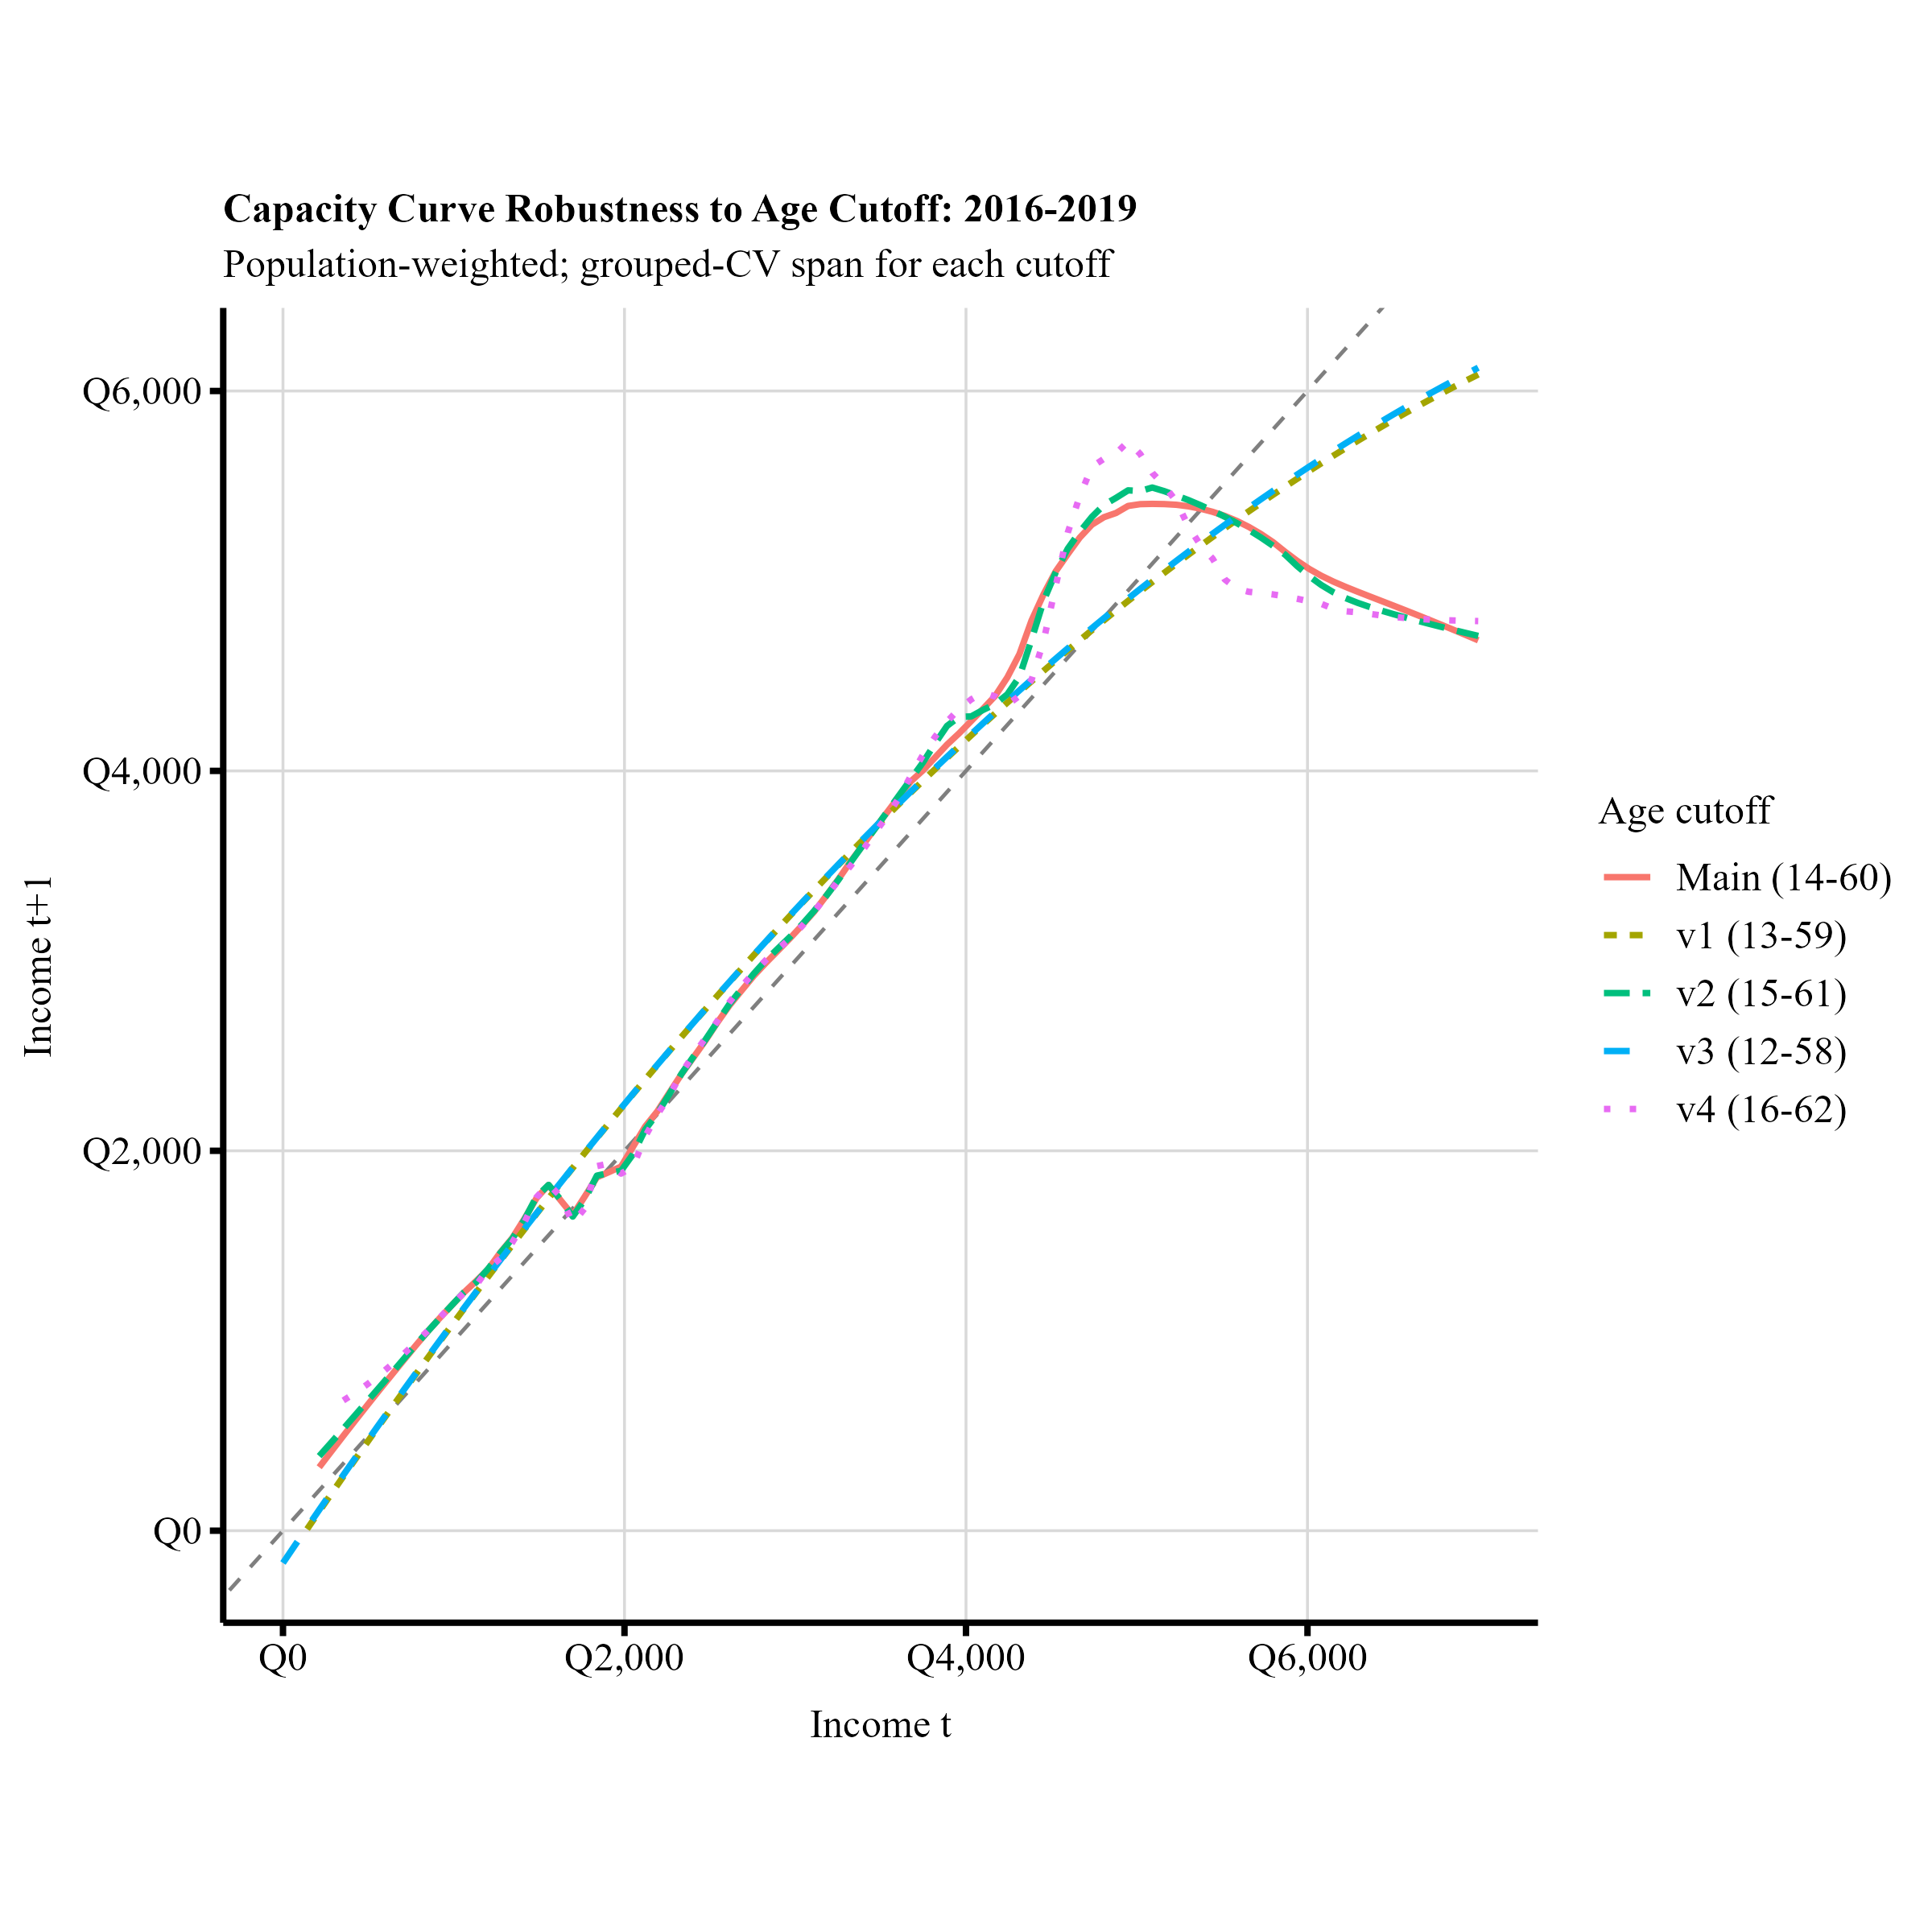
\includegraphics[trim={0.72bp 50.40bp 4.32bp 50.64bp},clip,width=0.90\linewidth,height=0.36\textheight,keepaspectratio]{figures/age-2016-2019-retuned.png}
\caption{Age-cutoff robustness, 2016-2019: reselected bandwidth.}
\label{fig:age-2016-2019-retuned}
\end{figure}

\begin{figure}[!htbp]
\singlespacing
\centering
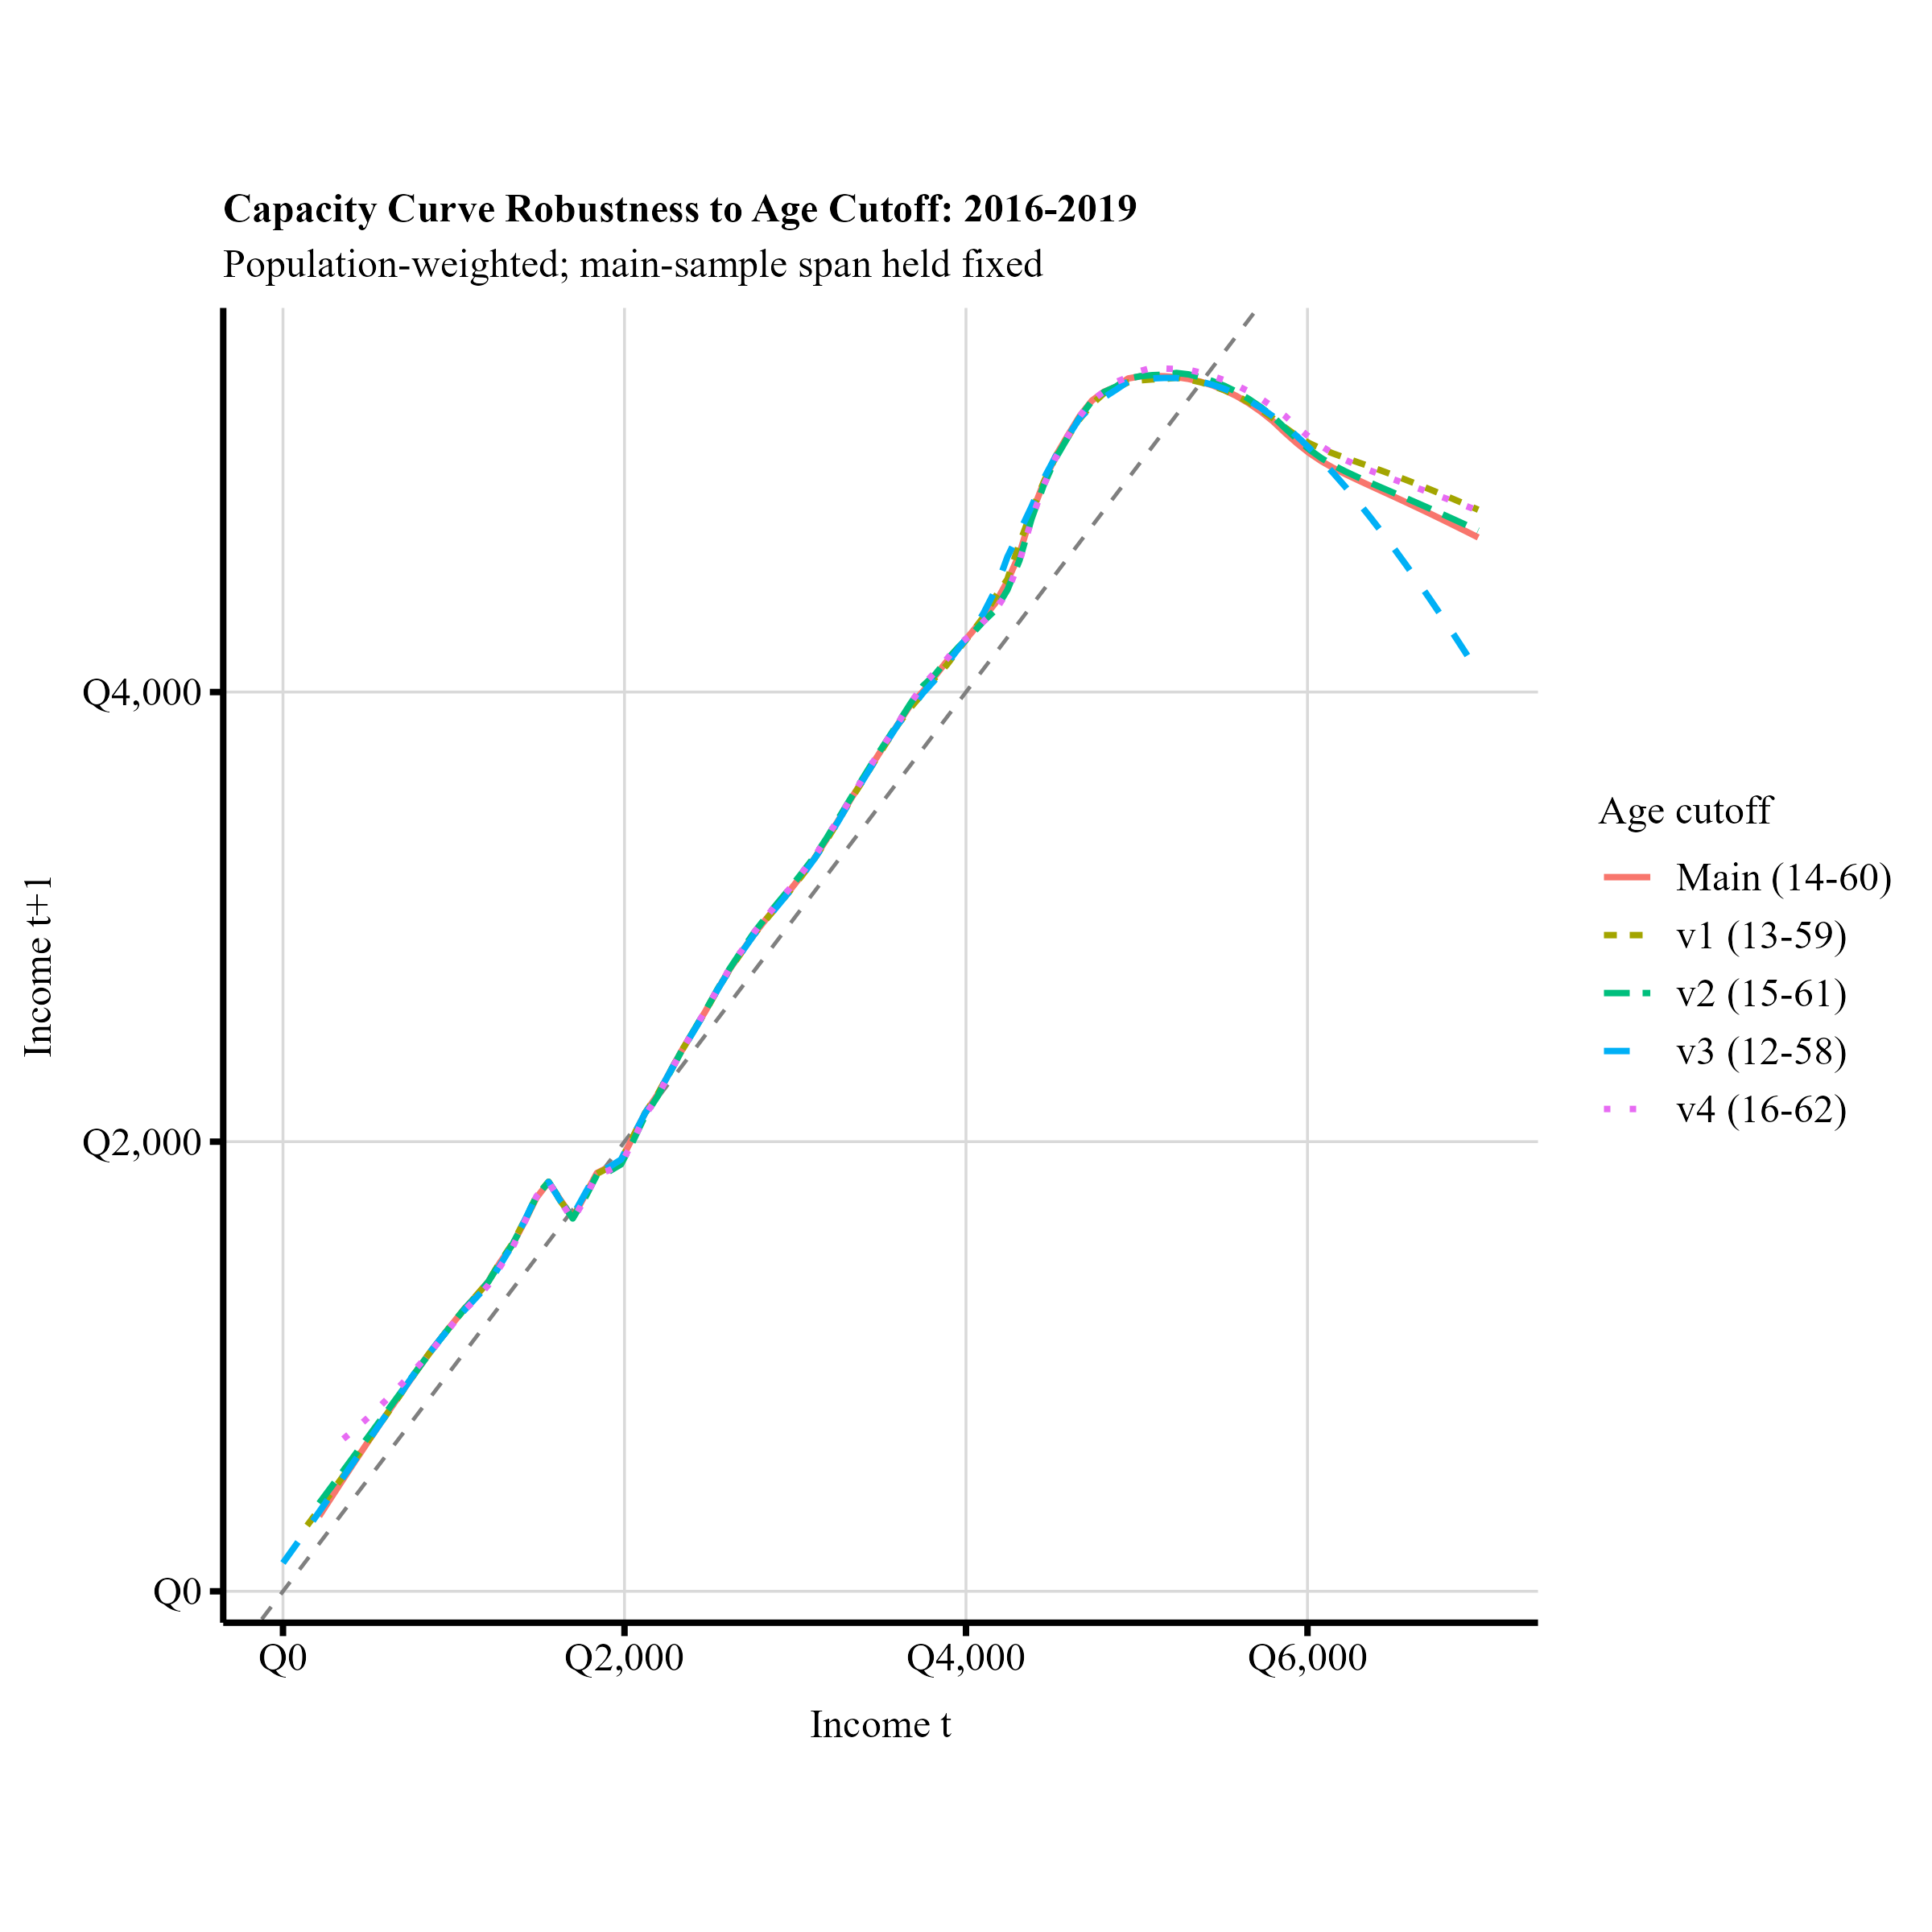
\includegraphics[trim={0.72bp 50.40bp 4.32bp 50.64bp},clip,width=0.90\linewidth,height=0.36\textheight,keepaspectratio]{figures/age-2016-2019-fixed.png}
\caption{Age-cutoff robustness, 2016-2019: fixed baseline bandwidth.}
\label{fig:age-2016-2019-fixed}
\end{figure}

\begin{figure}[!htbp]
\singlespacing
\centering
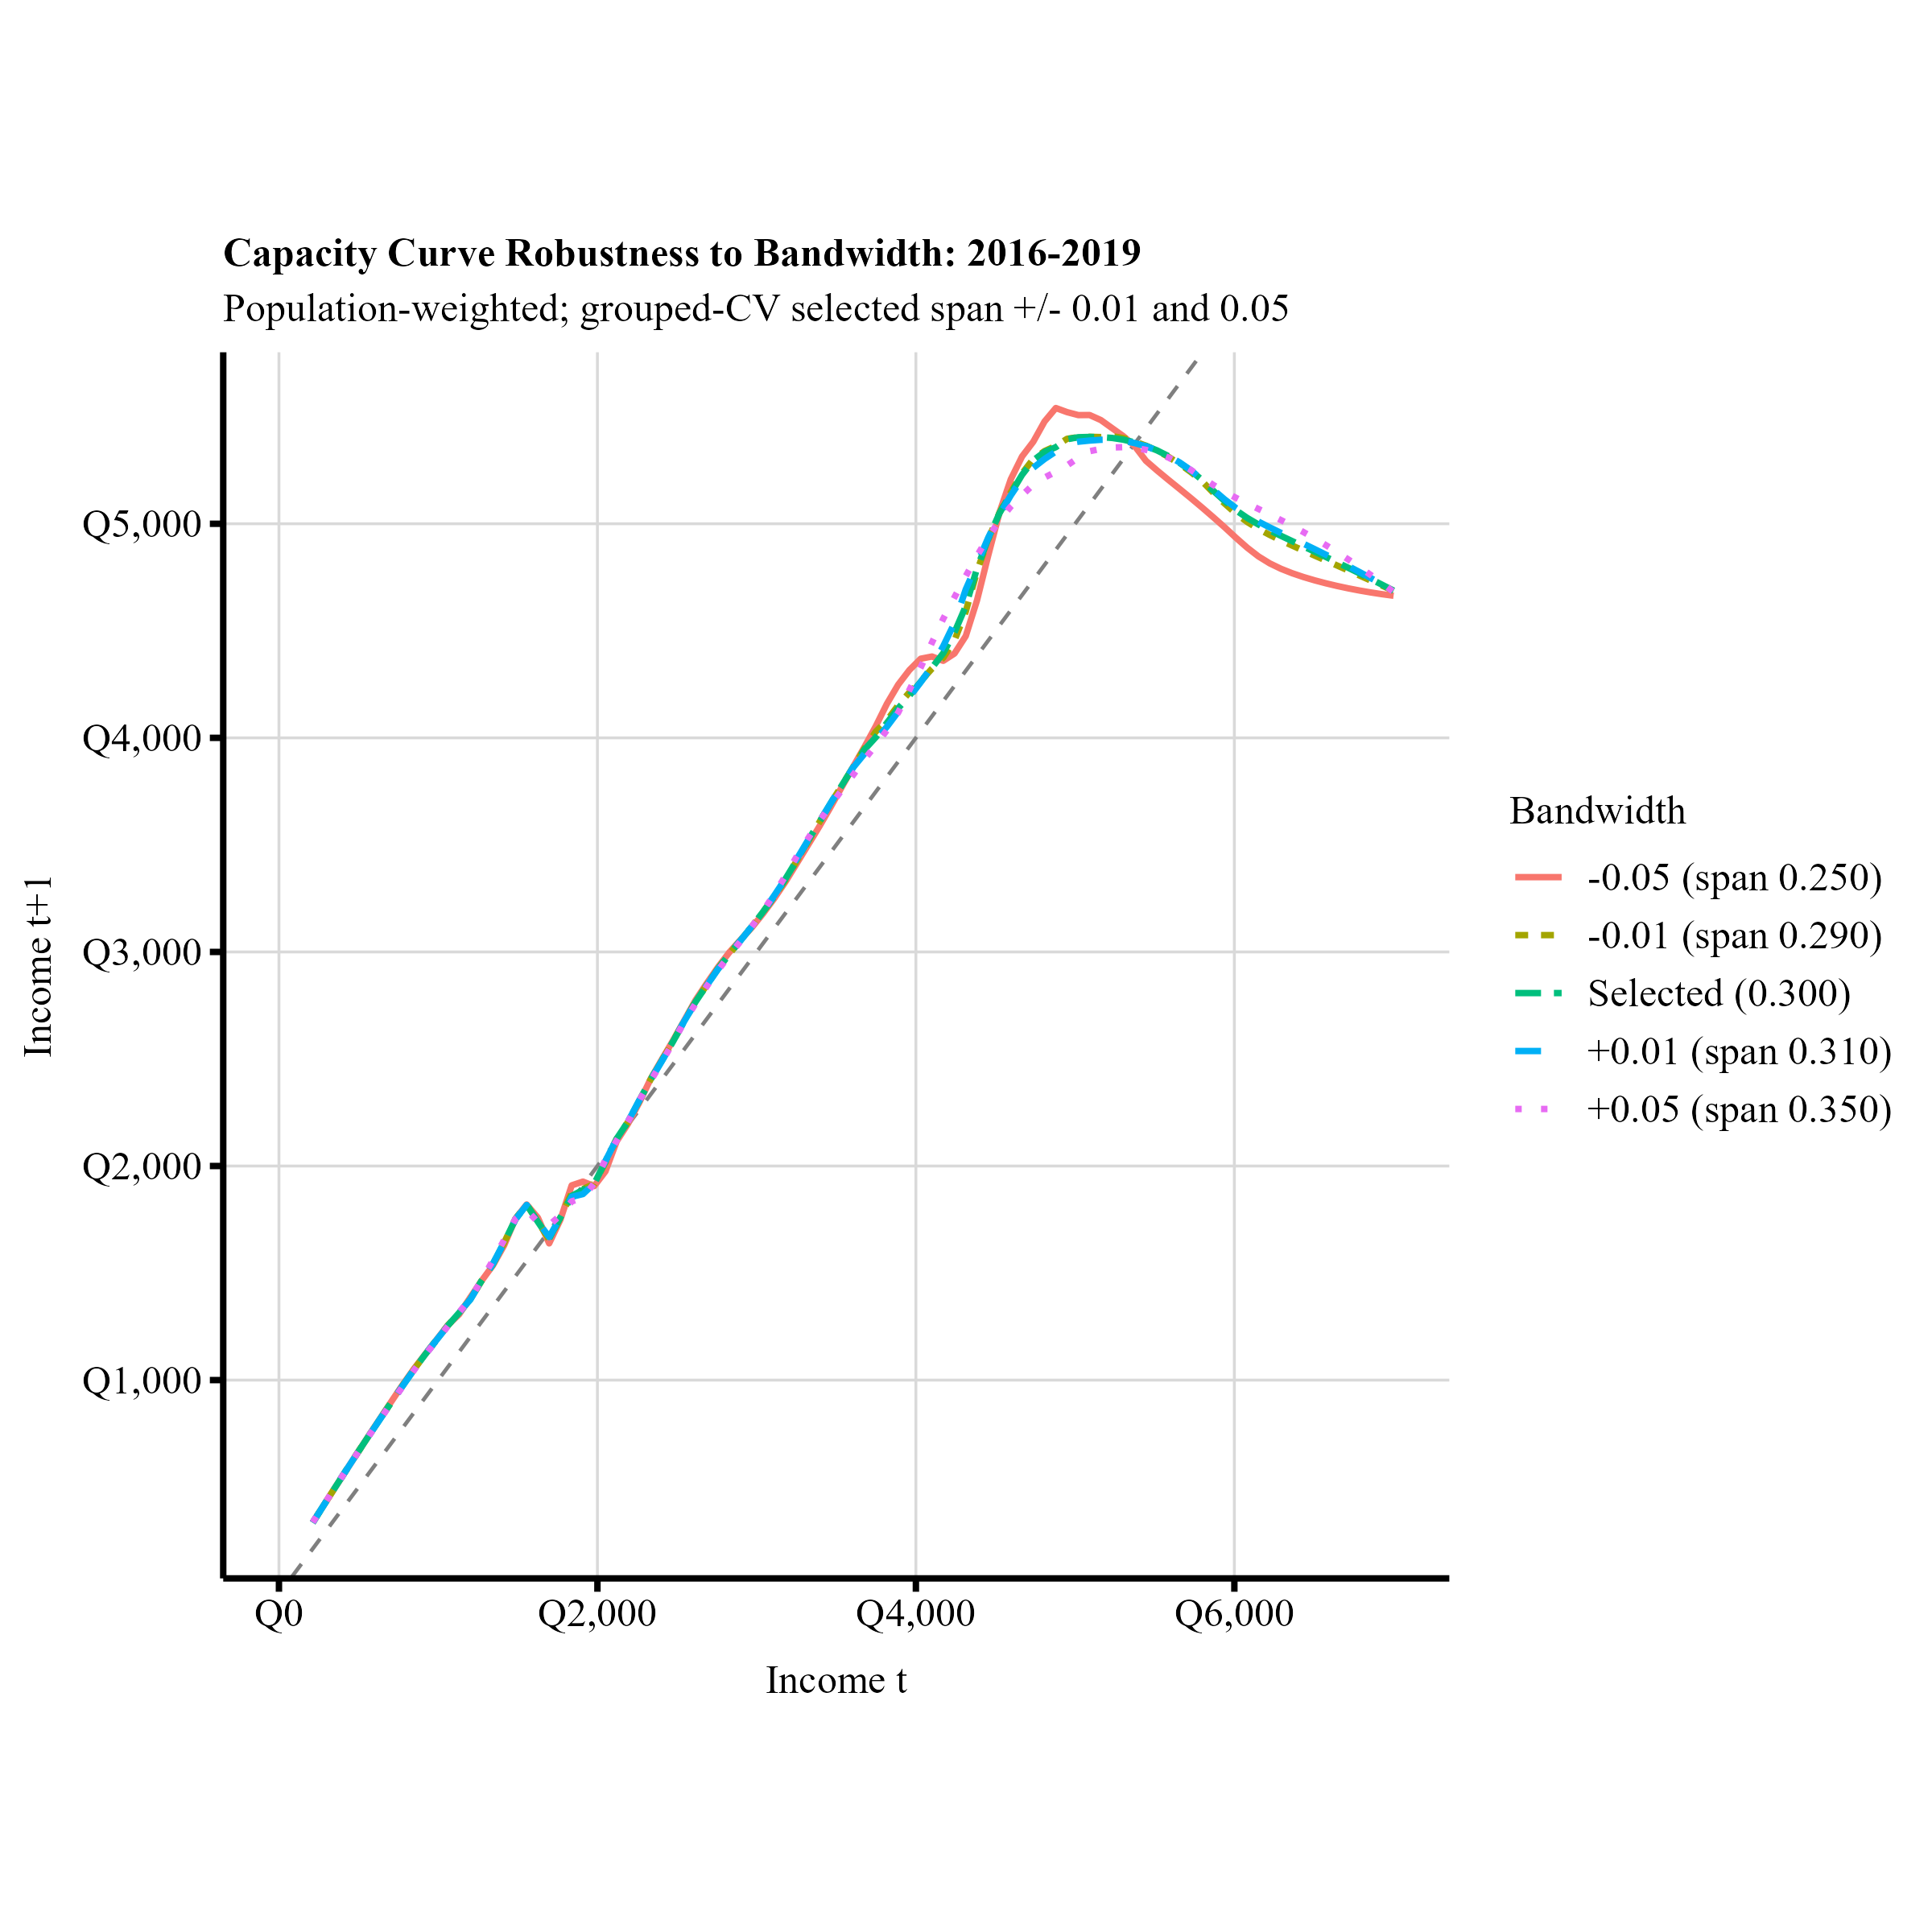
\includegraphics[trim={0.72bp 61.92bp 4.32bp 62.16bp},clip,width=0.90\linewidth,height=0.36\textheight,keepaspectratio]{figures/bandwidth-2016-2019.png}
\caption{Bandwidth robustness, 2016-2019.}
\label{fig:bandwidth-2016-2019}
\end{figure}

\begin{figure}[!htbp]
\singlespacing
\centering
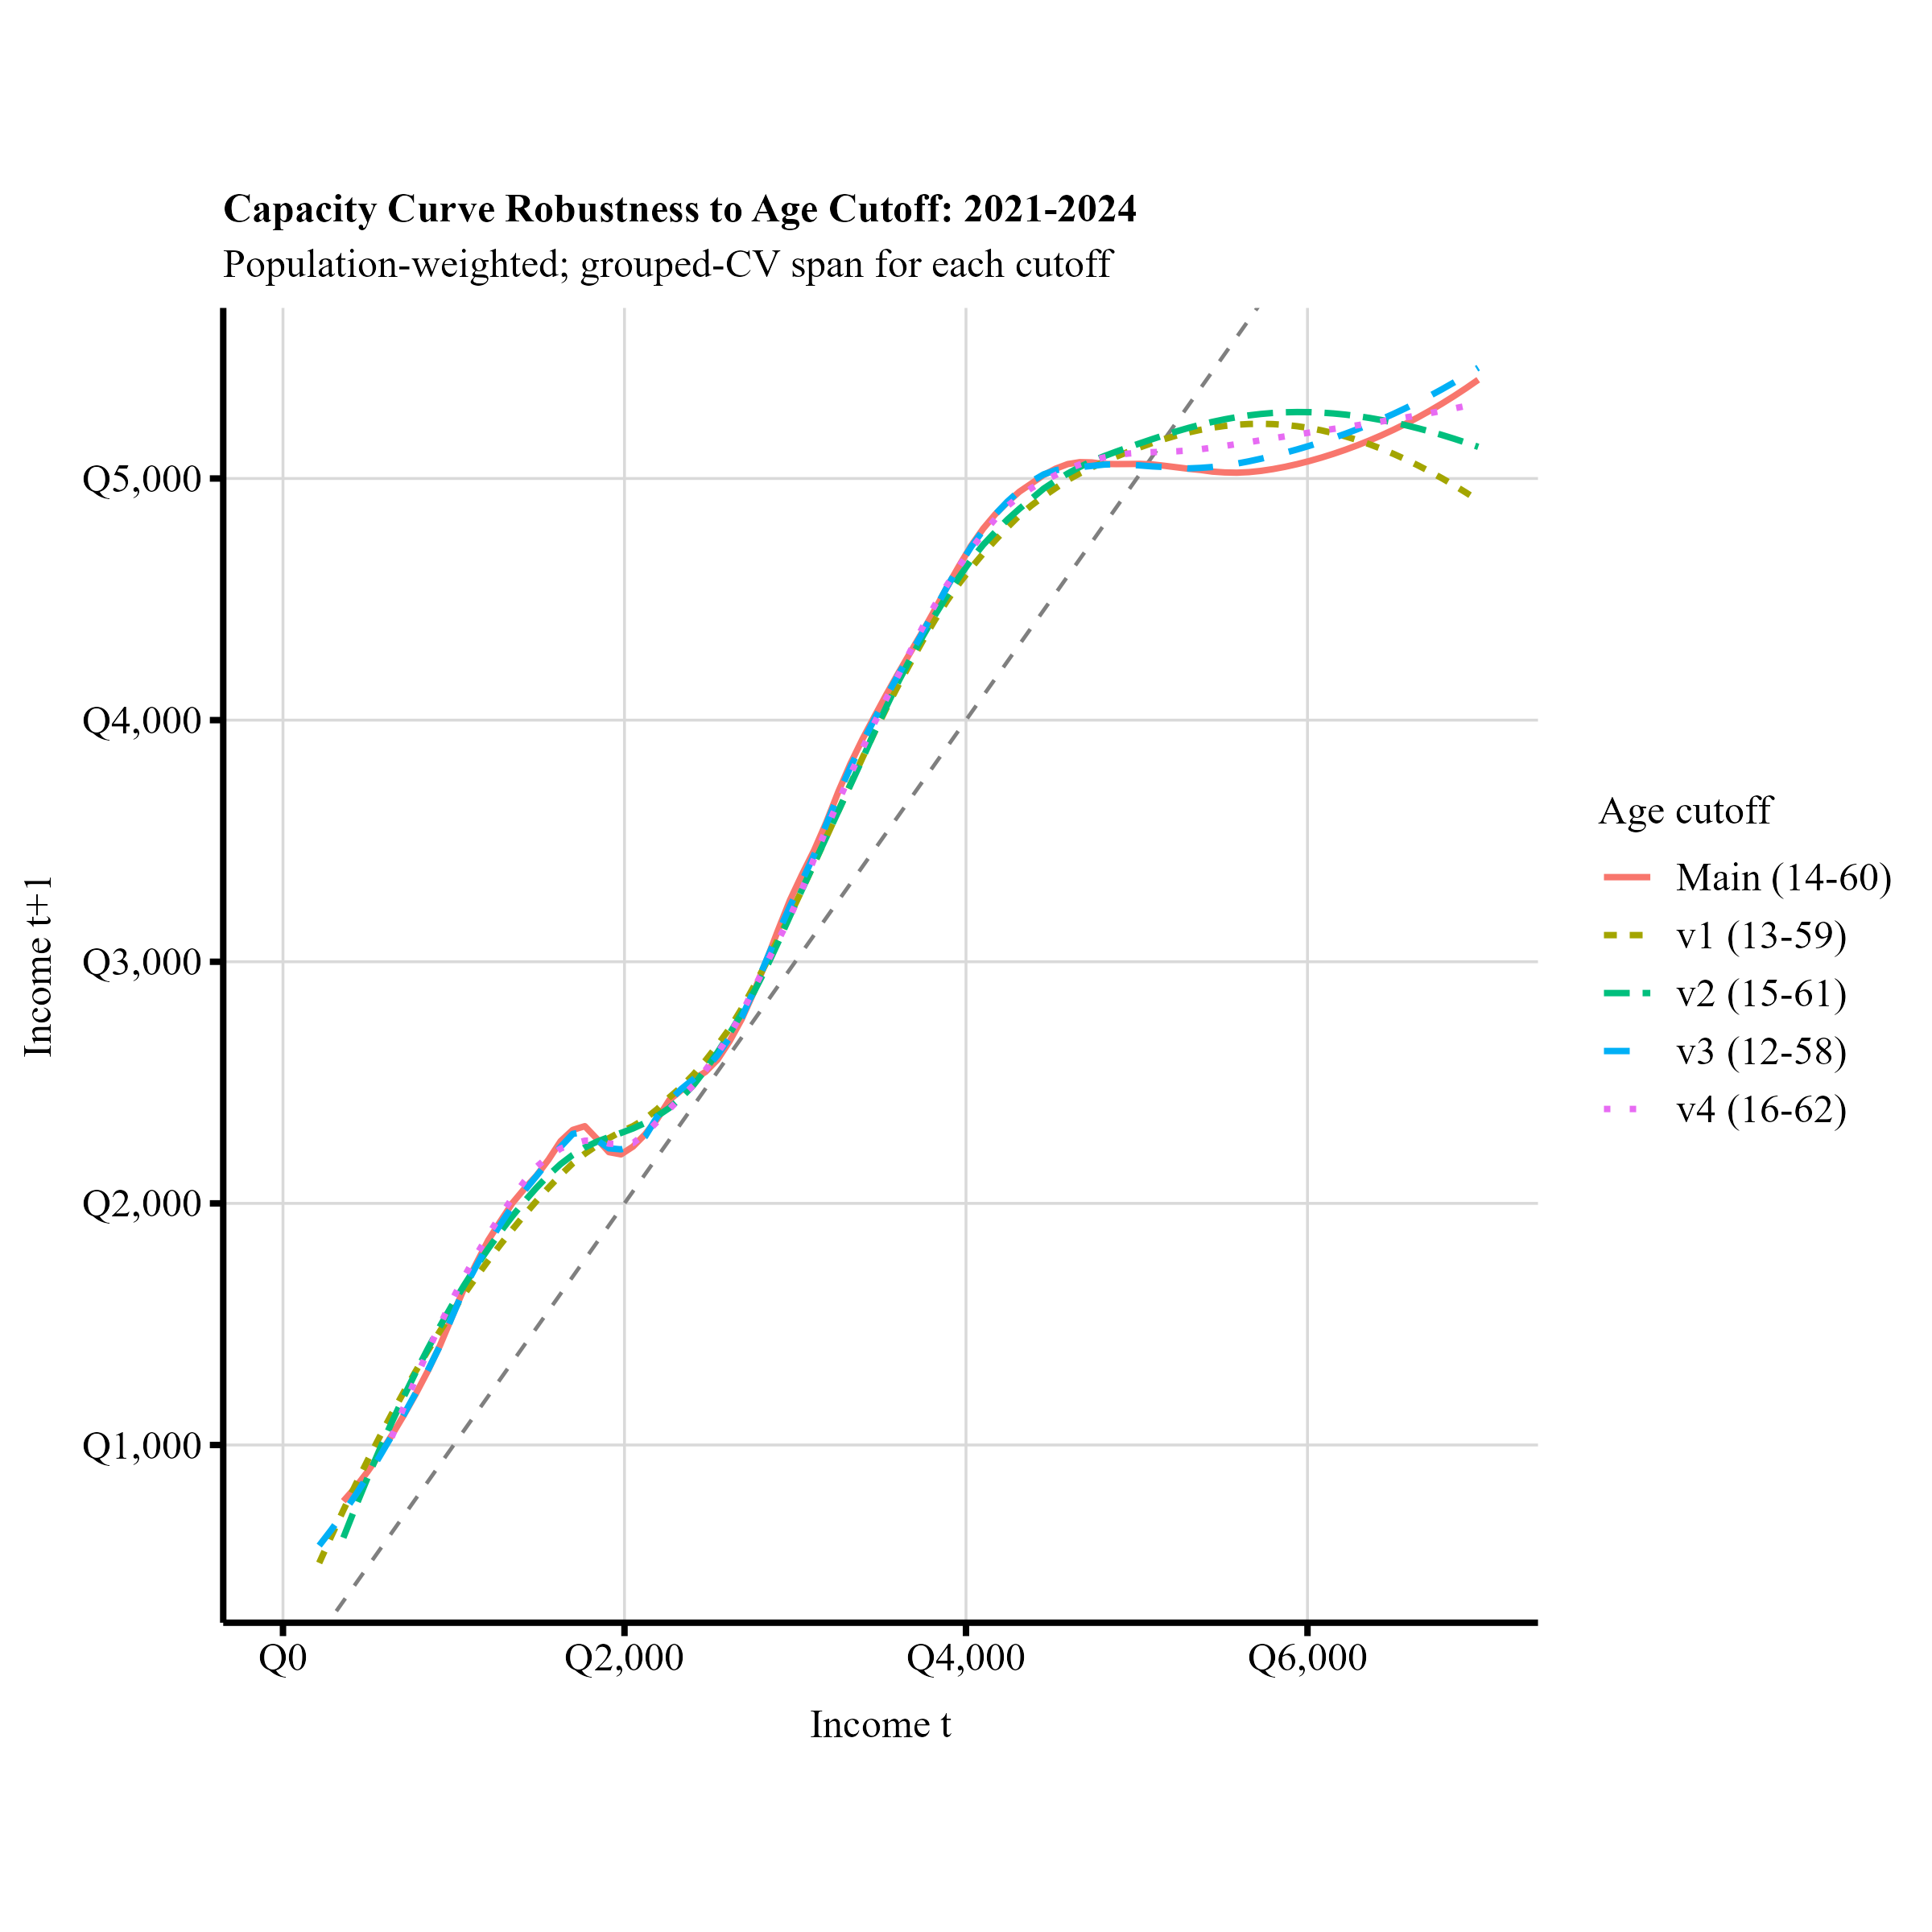
\includegraphics[trim={0.72bp 50.40bp 4.32bp 50.64bp},clip,width=0.90\linewidth,height=0.36\textheight,keepaspectratio]{figures/age-2021-2024-retuned.png}
\caption{Age-cutoff robustness, 2021-2024: reselected bandwidth.}
\label{fig:age-2021-2024-retuned}
\end{figure}

\begin{figure}[!htbp]
\singlespacing
\centering
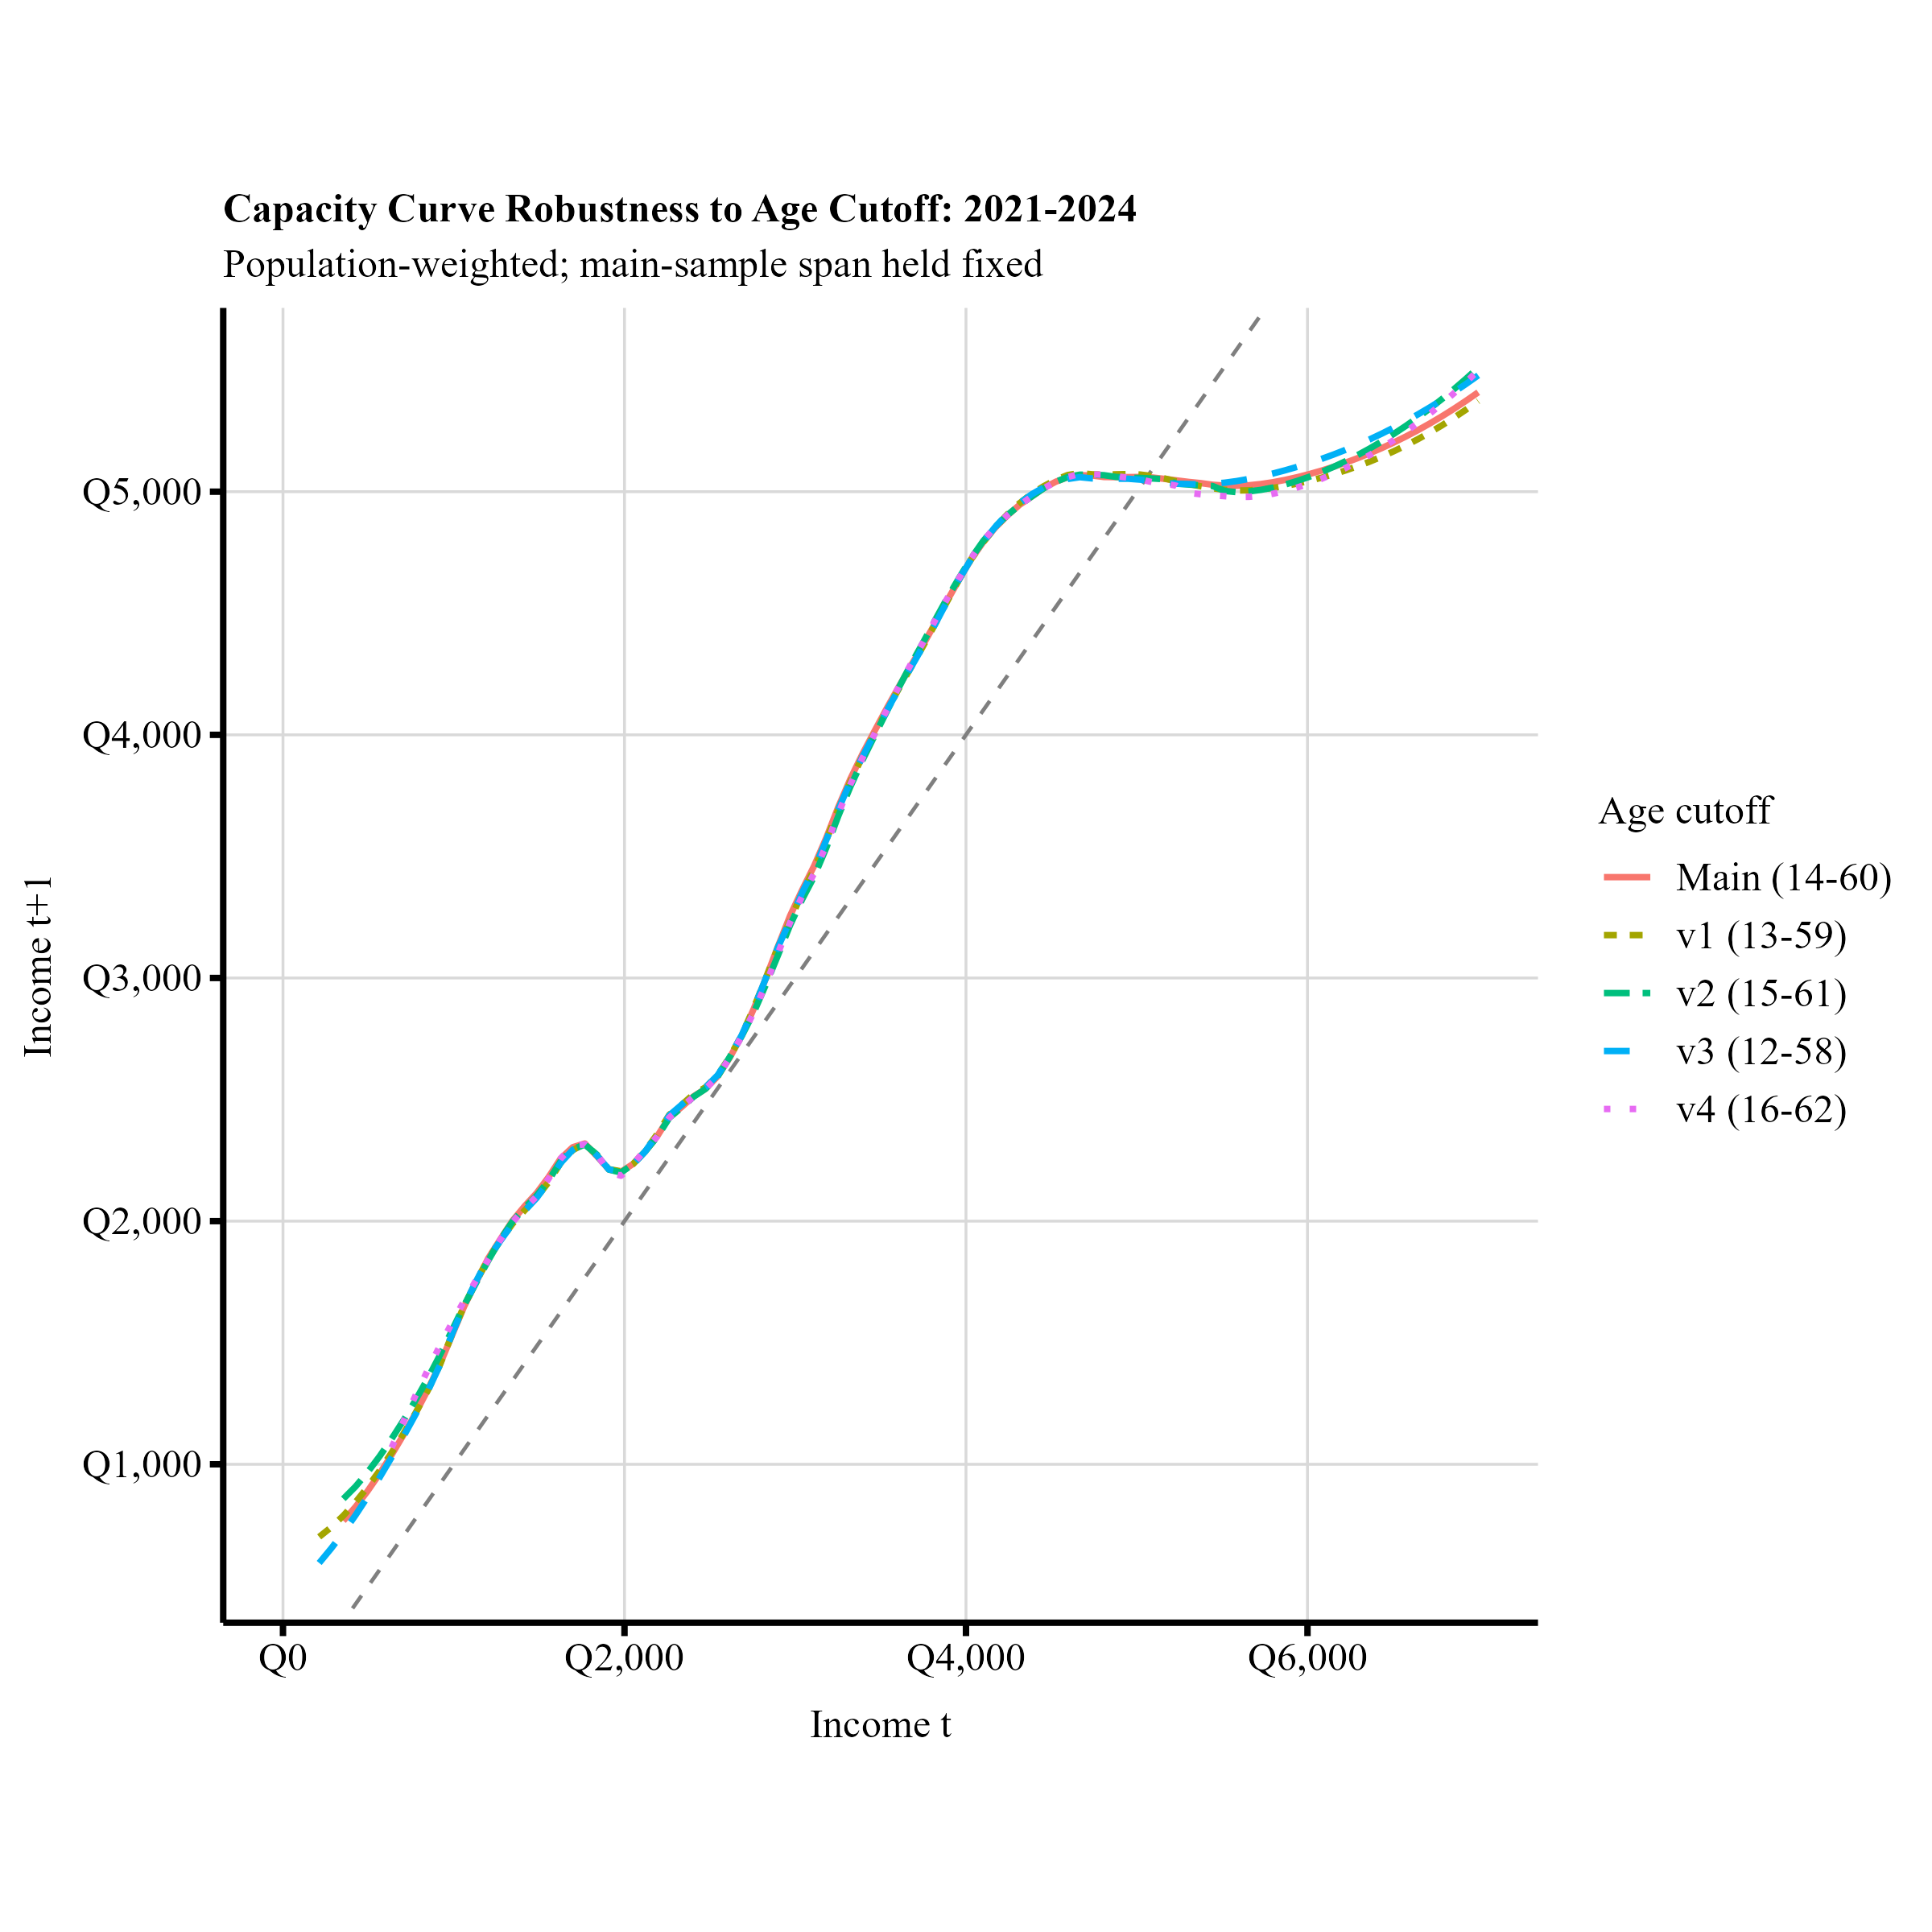
\includegraphics[trim={0.72bp 50.40bp 4.32bp 50.64bp},clip,width=0.90\linewidth,height=0.36\textheight,keepaspectratio]{figures/age-2021-2024-fixed.png}
\caption{Age-cutoff robustness, 2021-2024: fixed baseline bandwidth.}
\label{fig:age-2021-2024-fixed}
\end{figure}

\begin{figure}[!htbp]
\singlespacing
\centering
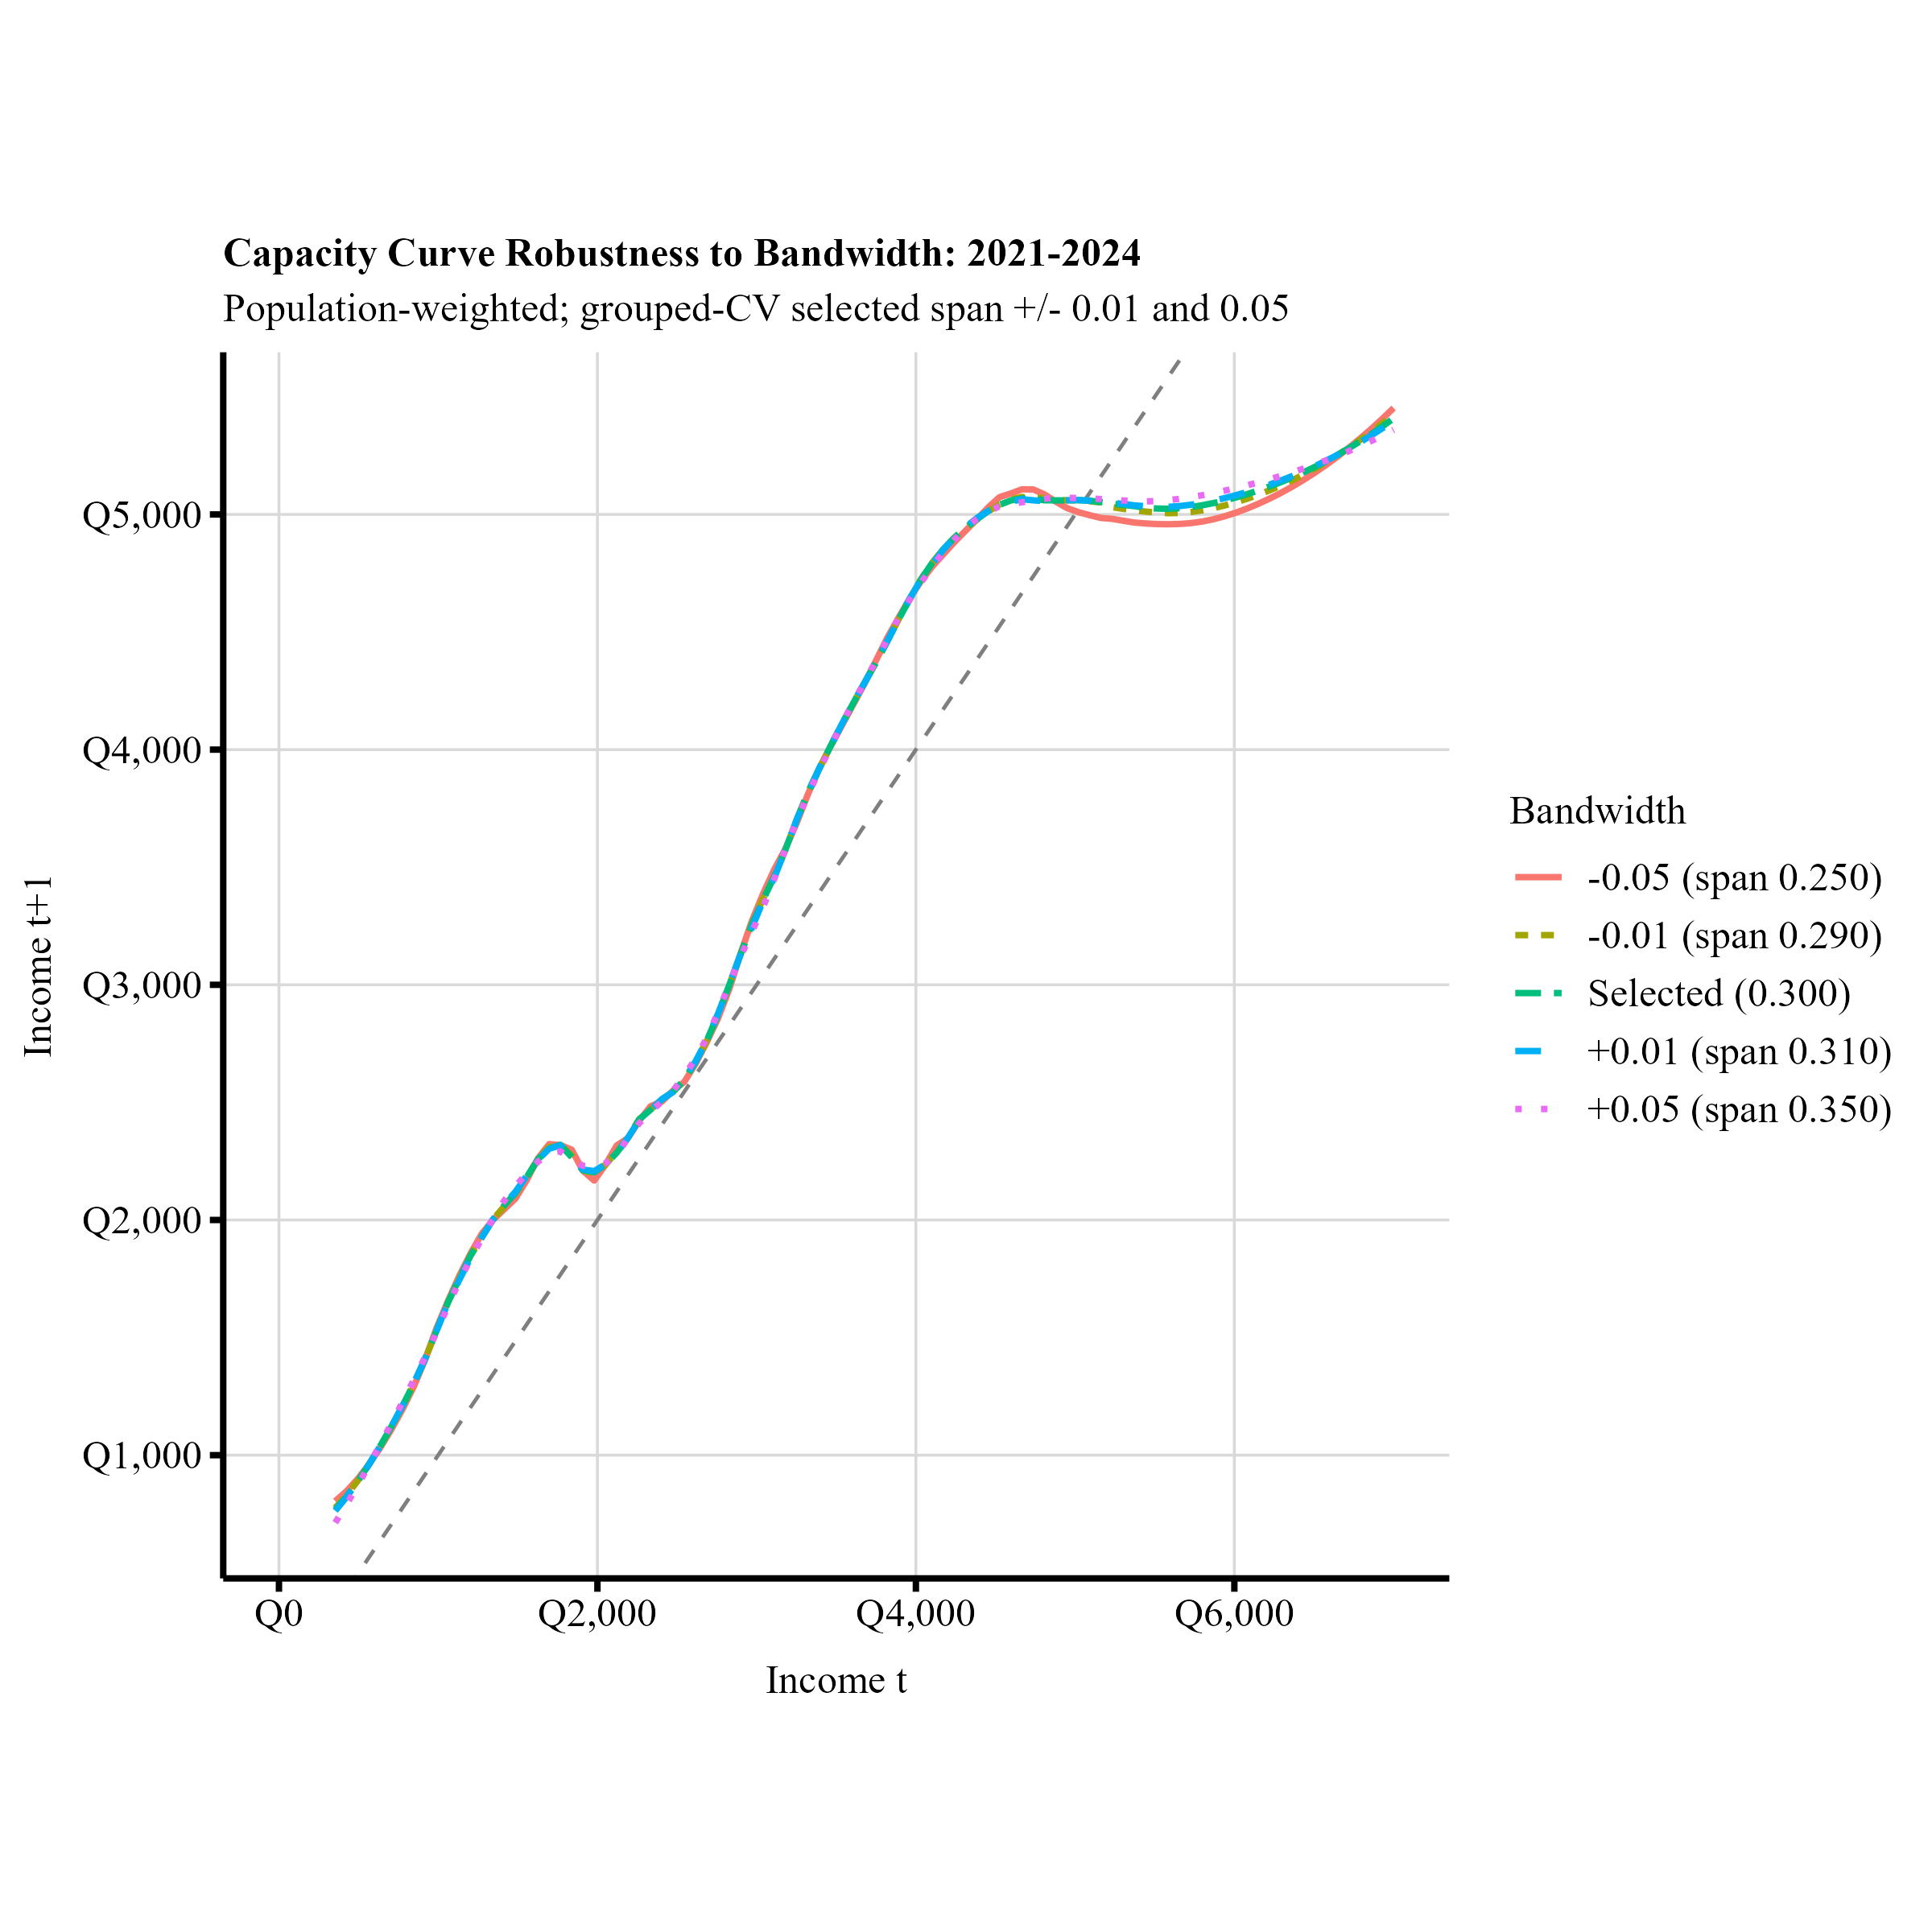
\includegraphics[trim={0.72bp 61.92bp 4.32bp 62.16bp},clip,width=0.90\linewidth,height=0.36\textheight,keepaspectratio]{figures/bandwidth-2021-2024.png}
\caption{Bandwidth robustness, 2021-2024.}
\label{fig:bandwidth-2021-2024}
\end{figure}

\section{Descriptive statistics}
\begingroup
\singlespacing
% Generated from project outputs. Do not edit by hand.
\begin{table}[!htbp]
\centering
\begin{threeparttable}
\caption{General-sample income moments at t in 2016-2019}
\label{tab:descriptive-2016-2019-moments-t1}
\small
\setlength{\tabcolsep}{4pt}
\renewcommand{\arraystretch}{1.15}
\begin{tabularx}{\linewidth}{@{}Xrrrrr@{}}
\toprule
Income & N & Mean & SD & Min & Max \\
\midrule
Labor income & 276 & 2,607.3 & 1,835.7 & 154.2 & 16,913.6 \\
Including in-kind & 276 & 2,687.2 & 1,829.6 & 169.2 & 16,921.9 \\
Including nonlabor & 276 & 2,822.6 & 1,947.4 & 169.2 & 17,829.7 \\
Including remittances & 276 & 2,866.2 & 1,954.8 & 169.2 & 17,836.7 \\
\bottomrule
\end{tabularx}
\begin{tablenotes}[flushleft]
\footnotesize
\item Monthly income in quetzales. Unweighted descriptive statistics of survey-weighted cohort means. N counts cohort-transition rows, not individuals or independent cohorts. SD is dispersion across cohort means, not the standard error of a mean.
\end{tablenotes}
\end{threeparttable}
\end{table}

% Generated from project outputs. Do not edit by hand.
\begin{table}[!htbp]
\centering
\begin{threeparttable}
\caption{General-sample income moments at t+1 in 2016-2019}
\label{tab:descriptive-2016-2019-moments-t2}
\small
\setlength{\tabcolsep}{4pt}
\renewcommand{\arraystretch}{1.15}
\begin{tabularx}{\linewidth}{@{}Xrrrrr@{}}
\toprule
Income & N & Mean & SD & Min & Max \\
\midrule
Labor income & 276 & 2,685.5 & 1,792.5 & 191.9 & 16,913.6 \\
Including in-kind & 276 & 2,753.5 & 1,786.4 & 199.5 & 16,921.9 \\
Including nonlabor & 276 & 2,867.7 & 1,869.6 & 213.3 & 17,829.7 \\
Including remittances & 276 & 2,907.3 & 1,870.3 & 213.3 & 17,836.7 \\
\bottomrule
\end{tabularx}
\begin{tablenotes}[flushleft]
\footnotesize
\item Monthly income in quetzales. Unweighted descriptive statistics of survey-weighted cohort means. N counts cohort-transition rows, not individuals or independent cohorts. SD is dispersion across cohort means, not the standard error of a mean.
\end{tablenotes}
\end{threeparttable}
\end{table}

% Generated from project outputs. Do not edit by hand.
\begin{table}[!htbp]
\centering
\begin{threeparttable}
\caption{General-sample income quantiles at t in 2016-2019}
\label{tab:descriptive-2016-2019-quantiles-t1}
\small
\setlength{\tabcolsep}{4pt}
\renewcommand{\arraystretch}{1.15}
\begin{tabularx}{\linewidth}{@{}Xrrr@{}}
\toprule
Income & P25 & Median & P75 \\
\midrule
Labor income & 1,432.5 & 1,772.9 & 3,930.8 \\
Including in-kind & 1,529.1 & 1,863.9 & 4,002.9 \\
Including nonlabor & 1,584.7 & 1,974.3 & 4,239.5 \\
Including remittances & 1,632.3 & 2,033.0 & 4,253.3 \\
\bottomrule
\end{tabularx}
\begin{tablenotes}[flushleft]
\footnotesize
\item Monthly income in quetzales. Unweighted descriptive statistics of survey-weighted cohort means. N counts cohort-transition rows, not individuals or independent cohorts. SD is dispersion across cohort means, not the standard error of a mean.
\end{tablenotes}
\end{threeparttable}
\end{table}

% Generated from project outputs. Do not edit by hand.
\begin{table}[!htbp]
\centering
\begin{threeparttable}
\caption{General-sample income quantiles at t+1 in 2016-2019}
\label{tab:descriptive-2016-2019-quantiles-t2}
\small
\setlength{\tabcolsep}{4pt}
\renewcommand{\arraystretch}{1.15}
\begin{tabularx}{\linewidth}{@{}Xrrr@{}}
\toprule
Income & P25 & Median & P75 \\
\midrule
Labor income & 1,458.0 & 1,871.8 & 3,939.8 \\
Including in-kind & 1,541.3 & 1,953.9 & 3,999.7 \\
Including nonlabor & 1,645.2 & 2,050.6 & 4,233.6 \\
Including remittances & 1,692.6 & 2,079.2 & 4,237.0 \\
\bottomrule
\end{tabularx}
\begin{tablenotes}[flushleft]
\footnotesize
\item Monthly income in quetzales. Unweighted descriptive statistics of survey-weighted cohort means. N counts cohort-transition rows, not individuals or independent cohorts. SD is dispersion across cohort means, not the standard error of a mean.
\end{tablenotes}
\end{threeparttable}
\end{table}

% Generated from project outputs. Do not edit by hand.
\begin{table}[!htbp]
\centering
\begin{threeparttable}
\caption{Labor income by subsample: 2016-2019}
\label{tab:descriptive-2016-2019-subsamples-y1}
\small
\setlength{\tabcolsep}{4pt}
\renewcommand{\arraystretch}{1.15}
\begin{tabularx}{\linewidth}{@{}Xrrrrr@{}}
\toprule
Sample & N & Mean t & SD t & Mean t+1 & SD t+1 \\
\midrule
General & 276 & 2,607.3 & 1,835.7 & 2,685.5 & 1,792.5 \\
Men & 276 & 2,907.2 & 2,200.0 & 2,964.6 & 2,130.7 \\
Women & 276 & 2,093.2 & 1,454.8 & 2,213.9 & 1,530.2 \\
Urban & 276 & 2,883.1 & 1,869.6 & 2,949.1 & 1,811.5 \\
Rural & 271 & 1,922.4 & 1,420.2 & 2,085.0 & 1,570.0 \\
Indigenous & 271 & 1,900.5 & 1,314.9 & 1,997.3 & 1,351.3 \\
Non-Indigenous & 276 & 2,822.2 & 1,887.4 & 2,915.5 & 1,853.0 \\
Bottom 99 percent & 276 & 2,372.6 & 1,368.1 & 2,453.3 & 1,351.8 \\
Bottom 90 percent & 276 & 1,935.6 & 942.6 & 2,004.9 & 920.7 \\
Bottom 50 percent & 272 & 990.0 & 423.3 & 1,060.9 & 431.5 \\
\bottomrule
\end{tabularx}
\begin{tablenotes}[flushleft]
\footnotesize
\item Monthly income in quetzales. Unweighted descriptive statistics of survey-weighted cohort means. N counts cohort-transition rows, not individuals or independent cohorts. SD is dispersion across cohort means, not the standard error of a mean. Both incomes must be observed. Subsamples overlap; bottom-income groups are cumulative.
\end{tablenotes}
\end{threeparttable}
\end{table}

% Generated from project outputs. Do not edit by hand.
\begin{table}[!htbp]
\centering
\begin{threeparttable}
\caption{Including in-kind by subsample: 2016-2019}
\label{tab:descriptive-2016-2019-subsamples-y2}
\small
\setlength{\tabcolsep}{4pt}
\renewcommand{\arraystretch}{1.15}
\begin{tabularx}{\linewidth}{@{}Xrrrrr@{}}
\toprule
Sample & N & Mean t & SD t & Mean t+1 & SD t+1 \\
\midrule
General & 276 & 2,687.2 & 1,829.6 & 2,753.5 & 1,786.4 \\
Men & 276 & 2,988.3 & 2,201.6 & 3,033.8 & 2,129.6 \\
Women & 276 & 2,173.3 & 1,434.8 & 2,283.4 & 1,512.2 \\
Urban & 276 & 2,961.9 & 1,862.7 & 3,015.5 & 1,804.7 \\
Rural & 271 & 2,003.5 & 1,419.3 & 2,156.1 & 1,569.4 \\
Indigenous & 271 & 1,972.3 & 1,303.3 & 2,058.9 & 1,340.6 \\
Non-Indigenous & 276 & 2,905.3 & 1,879.7 & 2,986.7 & 1,845.5 \\
Bottom 99 percent & 276 & 2,451.8 & 1,362.1 & 2,520.7 & 1,346.0 \\
Bottom 90 percent & 276 & 2,013.5 & 934.9 & 2,070.3 & 913.9 \\
Bottom 50 percent & 272 & 1,063.5 & 426.5 & 1,124.4 & 439.3 \\
\bottomrule
\end{tabularx}
\begin{tablenotes}[flushleft]
\footnotesize
\item Monthly income in quetzales. Unweighted descriptive statistics of survey-weighted cohort means. N counts cohort-transition rows, not individuals or independent cohorts. SD is dispersion across cohort means, not the standard error of a mean. Both incomes must be observed. Subsamples overlap; bottom-income groups are cumulative.
\end{tablenotes}
\end{threeparttable}
\end{table}

% Generated from project outputs. Do not edit by hand.
\begin{table}[!htbp]
\centering
\begin{threeparttable}
\caption{Including nonlabor by subsample: 2016-2019}
\label{tab:descriptive-2016-2019-subsamples-y3}
\small
\setlength{\tabcolsep}{4pt}
\renewcommand{\arraystretch}{1.15}
\begin{tabularx}{\linewidth}{@{}Xrrrrr@{}}
\toprule
Sample & N & Mean t & SD t & Mean t+1 & SD t+1 \\
\midrule
General & 276 & 2,822.6 & 1,947.4 & 2,867.7 & 1,869.6 \\
Men & 276 & 3,133.9 & 2,350.7 & 3,156.9 & 2,241.0 \\
Women & 276 & 2,289.0 & 1,527.4 & 2,383.1 & 1,569.6 \\
Urban & 276 & 3,103.9 & 1,990.7 & 3,131.6 & 1,889.2 \\
Rural & 271 & 2,108.7 & 1,478.6 & 2,248.4 & 1,609.0 \\
Indigenous & 271 & 2,083.8 & 1,425.3 & 2,144.7 & 1,400.6 \\
Non-Indigenous & 276 & 3,049.3 & 1,993.5 & 3,110.3 & 1,929.8 \\
Bottom 99 percent & 276 & 2,574.8 & 1,445.5 & 2,628.5 & 1,408.8 \\
Bottom 90 percent & 276 & 2,134.2 & 1,027.0 & 2,177.3 & 988.3 \\
Bottom 50 percent & 272 & 1,193.1 & 531.3 & 1,247.5 & 533.0 \\
\bottomrule
\end{tabularx}
\begin{tablenotes}[flushleft]
\footnotesize
\item Monthly income in quetzales. Unweighted descriptive statistics of survey-weighted cohort means. N counts cohort-transition rows, not individuals or independent cohorts. SD is dispersion across cohort means, not the standard error of a mean. Both incomes must be observed. Subsamples overlap; bottom-income groups are cumulative.
\end{tablenotes}
\end{threeparttable}
\end{table}

% Generated from project outputs. Do not edit by hand.
\begin{table}[!htbp]
\centering
\begin{threeparttable}
\caption{Including remittances by subsample: 2016-2019}
\label{tab:descriptive-2016-2019-subsamples-y4}
\small
\setlength{\tabcolsep}{4pt}
\renewcommand{\arraystretch}{1.15}
\begin{tabularx}{\linewidth}{@{}Xrrrrr@{}}
\toprule
Sample & N & Mean t & SD t & Mean t+1 & SD t+1 \\
\midrule
General & 276 & 2,866.2 & 1,954.8 & 2,907.3 & 1,870.3 \\
Men & 276 & 3,165.2 & 2,352.4 & 3,185.5 & 2,238.1 \\
Women & 276 & 2,353.0 & 1,541.1 & 2,441.5 & 1,573.3 \\
Urban & 276 & 3,143.4 & 1,995.0 & 3,165.8 & 1,890.8 \\
Rural & 271 & 2,170.9 & 1,515.3 & 2,297.9 & 1,621.2 \\
Indigenous & 271 & 2,132.5 & 1,426.9 & 2,180.2 & 1,395.6 \\
Non-Indigenous & 276 & 3,087.8 & 2,004.1 & 3,146.2 & 1,934.4 \\
Bottom 99 percent & 276 & 2,618.4 & 1,455.7 & 2,668.1 & 1,412.6 \\
Bottom 90 percent & 276 & 2,176.8 & 1,036.0 & 2,214.8 & 989.2 \\
Bottom 50 percent & 272 & 1,251.3 & 564.8 & 1,299.7 & 548.7 \\
\bottomrule
\end{tabularx}
\begin{tablenotes}[flushleft]
\footnotesize
\item Monthly income in quetzales. Unweighted descriptive statistics of survey-weighted cohort means. N counts cohort-transition rows, not individuals or independent cohorts. SD is dispersion across cohort means, not the standard error of a mean. Both incomes must be observed. Subsamples overlap; bottom-income groups are cumulative.
\end{tablenotes}
\end{threeparttable}
\end{table}

% Generated from project outputs. Do not edit by hand.
\begin{table}[!htbp]
\centering
\begin{threeparttable}
\caption{General-sample income moments at t in 2016-2024}
\label{tab:descriptive-2016-2024-moments-t1}
\small
\setlength{\tabcolsep}{4pt}
\renewcommand{\arraystretch}{1.15}
\begin{tabularx}{\linewidth}{@{}Xrrrrr@{}}
\toprule
Income & N & Mean & SD & Min & Max \\
\midrule
Labor income & 552 & 2,712.6 & 1,677.9 & 154.2 & 16,913.6 \\
Including in-kind & 552 & 2,780.6 & 1,673.9 & 169.2 & 16,921.9 \\
Including nonlabor & 552 & 2,913.6 & 1,786.2 & 169.2 & 17,829.7 \\
Including remittances & 552 & 2,970.8 & 1,798.4 & 169.2 & 17,836.7 \\
\bottomrule
\end{tabularx}
\begin{tablenotes}[flushleft]
\footnotesize
\item Monthly income in quetzales. Unweighted descriptive statistics of survey-weighted cohort means. N counts cohort-transition rows, not individuals or independent cohorts. SD is dispersion across cohort means, not the standard error of a mean. Six annual transitions are pooled; the 2019-2021 gap is excluded.
\end{tablenotes}
\end{threeparttable}
\end{table}

% Generated from project outputs. Do not edit by hand.
\begin{table}[!htbp]
\centering
\begin{threeparttable}
\caption{General-sample income moments at t+1 in 2016-2024}
\label{tab:descriptive-2016-2024-moments-t2}
\small
\setlength{\tabcolsep}{4pt}
\renewcommand{\arraystretch}{1.15}
\begin{tabularx}{\linewidth}{@{}Xrrrrr@{}}
\toprule
Income & N & Mean & SD & Min & Max \\
\midrule
Labor income & 552 & 2,907.8 & 1,692.0 & 191.9 & 16,913.6 \\
Including in-kind & 552 & 2,973.6 & 1,692.8 & 199.5 & 16,921.9 \\
Including nonlabor & 552 & 3,111.6 & 1,795.1 & 213.3 & 17,829.7 \\
Including remittances & 552 & 3,175.9 & 1,809.5 & 213.3 & 17,836.7 \\
\bottomrule
\end{tabularx}
\begin{tablenotes}[flushleft]
\footnotesize
\item Monthly income in quetzales. Unweighted descriptive statistics of survey-weighted cohort means. N counts cohort-transition rows, not individuals or independent cohorts. SD is dispersion across cohort means, not the standard error of a mean. Six annual transitions are pooled; the 2019-2021 gap is excluded.
\end{tablenotes}
\end{threeparttable}
\end{table}

% Generated from project outputs. Do not edit by hand.
\begin{table}[!htbp]
\centering
\begin{threeparttable}
\caption{General-sample income quantiles at t in 2016-2024}
\label{tab:descriptive-2016-2024-quantiles-t1}
\small
\setlength{\tabcolsep}{4pt}
\renewcommand{\arraystretch}{1.15}
\begin{tabularx}{\linewidth}{@{}Xrrr@{}}
\toprule
Income & P25 & Median & P75 \\
\midrule
Labor income & 1,534.3 & 2,148.3 & 3,982.5 \\
Including in-kind & 1,617.5 & 2,196.9 & 4,033.2 \\
Including nonlabor & 1,700.3 & 2,278.9 & 4,269.2 \\
Including remittances & 1,746.4 & 2,378.2 & 4,325.2 \\
\bottomrule
\end{tabularx}
\begin{tablenotes}[flushleft]
\footnotesize
\item Monthly income in quetzales. Unweighted descriptive statistics of survey-weighted cohort means. N counts cohort-transition rows, not individuals or independent cohorts. SD is dispersion across cohort means, not the standard error of a mean. Six annual transitions are pooled; the 2019-2021 gap is excluded.
\end{tablenotes}
\end{threeparttable}
\end{table}

% Generated from project outputs. Do not edit by hand.
\begin{table}[!htbp]
\centering
\begin{threeparttable}
\caption{General-sample income quantiles at t+1 in 2016-2024}
\label{tab:descriptive-2016-2024-quantiles-t2}
\small
\setlength{\tabcolsep}{4pt}
\renewcommand{\arraystretch}{1.15}
\begin{tabularx}{\linewidth}{@{}Xrrr@{}}
\toprule
Income & P25 & Median & P75 \\
\midrule
Labor income & 1,646.5 & 2,299.5 & 4,157.8 \\
Including in-kind & 1,704.8 & 2,350.9 & 4,225.3 \\
Including nonlabor & 1,783.4 & 2,452.7 & 4,432.3 \\
Including remittances & 1,850.3 & 2,560.1 & 4,470.7 \\
\bottomrule
\end{tabularx}
\begin{tablenotes}[flushleft]
\footnotesize
\item Monthly income in quetzales. Unweighted descriptive statistics of survey-weighted cohort means. N counts cohort-transition rows, not individuals or independent cohorts. SD is dispersion across cohort means, not the standard error of a mean. Six annual transitions are pooled; the 2019-2021 gap is excluded.
\end{tablenotes}
\end{threeparttable}
\end{table}

% Generated from project outputs. Do not edit by hand.
\begin{table}[!htbp]
\centering
\begin{threeparttable}
\caption{Labor income by subsample: 2016-2024}
\label{tab:descriptive-2016-2024-subsamples-y1}
\small
\setlength{\tabcolsep}{4pt}
\renewcommand{\arraystretch}{1.15}
\begin{tabularx}{\linewidth}{@{}Xrrrrr@{}}
\toprule
Sample & N & Mean t & SD t & Mean t+1 & SD t+1 \\
\midrule
General & 552 & 2,712.6 & 1,677.9 & 2,907.8 & 1,692.0 \\
Men & 552 & 3,046.6 & 1,937.0 & 3,264.3 & 1,932.0 \\
Women & 552 & 2,162.5 & 1,498.6 & 2,353.7 & 1,577.9 \\
Urban & 552 & 2,962.4 & 1,721.1 & 3,141.0 & 1,716.7 \\
Rural & 547 & 2,208.2 & 1,556.0 & 2,436.6 & 1,695.7 \\
Indigenous & 547 & 2,191.5 & 1,587.2 & 2,465.0 & 1,666.5 \\
Non-Indigenous & 460 & 2,882.8 & 1,765.7 & 3,023.1 & 1,726.2 \\
Bottom 99 percent & 552 & 2,507.0 & 1,332.9 & 2,694.0 & 1,349.4 \\
Bottom 90 percent & 552 & 2,057.7 & 921.3 & 2,207.8 & 916.1 \\
Bottom 50 percent & 548 & 1,101.8 & 465.6 & 1,194.7 & 460.4 \\
\bottomrule
\end{tabularx}
\begin{tablenotes}[flushleft]
\footnotesize
\item Monthly income in quetzales. Unweighted descriptive statistics of survey-weighted cohort means. N counts cohort-transition rows, not individuals or independent cohorts. SD is dispersion across cohort means, not the standard error of a mean. Six annual transitions are pooled; the 2019-2021 gap is excluded. Both incomes must be observed. Subsamples overlap; bottom-income groups are cumulative.
\end{tablenotes}
\end{threeparttable}
\end{table}

% Generated from project outputs. Do not edit by hand.
\begin{table}[!htbp]
\centering
\begin{threeparttable}
\caption{Including in-kind by subsample: 2016-2024}
\label{tab:descriptive-2016-2024-subsamples-y2}
\small
\setlength{\tabcolsep}{4pt}
\renewcommand{\arraystretch}{1.15}
\begin{tabularx}{\linewidth}{@{}Xrrrrr@{}}
\toprule
Sample & N & Mean t & SD t & Mean t+1 & SD t+1 \\
\midrule
General & 552 & 2,780.6 & 1,673.9 & 2,973.6 & 1,692.8 \\
Men & 552 & 3,117.5 & 1,940.7 & 3,336.1 & 1,938.1 \\
Women & 552 & 2,227.4 & 1,482.3 & 2,412.6 & 1,569.9 \\
Urban & 552 & 3,027.9 & 1,717.1 & 3,205.0 & 1,717.4 \\
Rural & 547 & 2,278.1 & 1,553.9 & 2,503.2 & 1,694.9 \\
Indigenous & 547 & 2,256.1 & 1,581.8 & 2,528.4 & 1,668.2 \\
Non-Indigenous & 460 & 2,955.7 & 1,758.2 & 3,084.1 & 1,722.5 \\
Bottom 99 percent & 552 & 2,573.7 & 1,327.4 & 2,757.2 & 1,346.8 \\
Bottom 90 percent & 552 & 2,122.3 & 914.5 & 2,267.6 & 913.0 \\
Bottom 50 percent & 548 & 1,162.2 & 463.2 & 1,247.3 & 459.9 \\
\bottomrule
\end{tabularx}
\begin{tablenotes}[flushleft]
\footnotesize
\item Monthly income in quetzales. Unweighted descriptive statistics of survey-weighted cohort means. N counts cohort-transition rows, not individuals or independent cohorts. SD is dispersion across cohort means, not the standard error of a mean. Six annual transitions are pooled; the 2019-2021 gap is excluded. Both incomes must be observed. Subsamples overlap; bottom-income groups are cumulative.
\end{tablenotes}
\end{threeparttable}
\end{table}

% Generated from project outputs. Do not edit by hand.
\begin{table}[!htbp]
\centering
\begin{threeparttable}
\caption{Including nonlabor by subsample: 2016-2024}
\label{tab:descriptive-2016-2024-subsamples-y3}
\small
\setlength{\tabcolsep}{4pt}
\renewcommand{\arraystretch}{1.15}
\begin{tabularx}{\linewidth}{@{}Xrrrrr@{}}
\toprule
Sample & N & Mean t & SD t & Mean t+1 & SD t+1 \\
\midrule
General & 552 & 2,913.6 & 1,786.2 & 3,111.6 & 1,795.1 \\
Men & 552 & 3,262.7 & 2,087.6 & 3,488.7 & 2,070.2 \\
Women & 552 & 2,339.7 & 1,568.3 & 2,528.4 & 1,649.8 \\
Urban & 552 & 3,159.5 & 1,834.8 & 3,338.9 & 1,815.6 \\
Rural & 547 & 2,391.7 & 1,635.4 & 2,634.6 & 1,817.8 \\
Indigenous & 547 & 2,371.6 & 1,690.4 & 2,643.2 & 1,765.7 \\
Non-Indigenous & 460 & 3,088.7 & 1,862.1 & 3,223.3 & 1,819.7 \\
Bottom 99 percent & 552 & 2,693.0 & 1,408.9 & 2,887.0 & 1,431.2 \\
Bottom 90 percent & 552 & 2,229.3 & 985.6 & 2,383.7 & 983.9 \\
Bottom 50 percent & 548 & 1,266.5 & 539.1 & 1,367.0 & 535.5 \\
\bottomrule
\end{tabularx}
\begin{tablenotes}[flushleft]
\footnotesize
\item Monthly income in quetzales. Unweighted descriptive statistics of survey-weighted cohort means. N counts cohort-transition rows, not individuals or independent cohorts. SD is dispersion across cohort means, not the standard error of a mean. Six annual transitions are pooled; the 2019-2021 gap is excluded. Both incomes must be observed. Subsamples overlap; bottom-income groups are cumulative.
\end{tablenotes}
\end{threeparttable}
\end{table}

% Generated from project outputs. Do not edit by hand.
\begin{table}[!htbp]
\centering
\begin{threeparttable}
\caption{Including remittances by subsample: 2016-2024}
\label{tab:descriptive-2016-2024-subsamples-y4}
\small
\setlength{\tabcolsep}{4pt}
\renewcommand{\arraystretch}{1.15}
\begin{tabularx}{\linewidth}{@{}Xrrrrr@{}}
\toprule
Sample & N & Mean t & SD t & Mean t+1 & SD t+1 \\
\midrule
General & 552 & 2,970.8 & 1,798.4 & 3,175.9 & 1,809.5 \\
Men & 552 & 3,305.1 & 2,098.5 & 3,537.8 & 2,083.8 \\
Women & 552 & 2,420.6 & 1,581.9 & 2,615.3 & 1,664.3 \\
Urban & 552 & 3,206.1 & 1,846.0 & 3,390.6 & 1,830.1 \\
Rural & 547 & 2,466.2 & 1,663.5 & 2,727.3 & 1,881.2 \\
Indigenous & 547 & 2,439.3 & 1,706.2 & 2,710.1 & 1,783.4 \\
Non-Indigenous & 460 & 3,135.4 & 1,875.2 & 3,273.9 & 1,830.1 \\
Bottom 99 percent & 552 & 2,750.2 & 1,424.1 & 2,950.9 & 1,448.9 \\
Bottom 90 percent & 552 & 2,285.0 & 1,002.1 & 2,444.7 & 1,001.6 \\
Bottom 50 percent & 548 & 1,329.9 & 565.4 & 1,436.2 & 562.6 \\
\bottomrule
\end{tabularx}
\begin{tablenotes}[flushleft]
\footnotesize
\item Monthly income in quetzales. Unweighted descriptive statistics of survey-weighted cohort means. N counts cohort-transition rows, not individuals or independent cohorts. SD is dispersion across cohort means, not the standard error of a mean. Six annual transitions are pooled; the 2019-2021 gap is excluded. Both incomes must be observed. Subsamples overlap; bottom-income groups are cumulative.
\end{tablenotes}
\end{threeparttable}
\end{table}

% Generated from project outputs. Do not edit by hand.
\begin{table}[!htbp]
\centering
\begin{threeparttable}
\caption{General-sample income moments at t in 2021-2024}
\label{tab:descriptive-2021-2024-moments-t1}
\small
\setlength{\tabcolsep}{4pt}
\renewcommand{\arraystretch}{1.15}
\begin{tabularx}{\linewidth}{@{}Xrrrrr@{}}
\toprule
Income & N & Mean & SD & Min & Max \\
\midrule
Labor income & 276 & 2,817.9 & 1,499.6 & 286.3 & 7,211.2 \\
Including in-kind & 276 & 2,873.9 & 1,499.7 & 299.9 & 7,263.4 \\
Including nonlabor & 276 & 3,004.7 & 1,607.3 & 353.5 & 7,796.2 \\
Including remittances & 276 & 3,075.5 & 1,623.8 & 353.5 & 7,861.0 \\
\bottomrule
\end{tabularx}
\begin{tablenotes}[flushleft]
\footnotesize
\item Monthly income in quetzales. Unweighted descriptive statistics of survey-weighted cohort means. N counts cohort-transition rows, not individuals or independent cohorts. SD is dispersion across cohort means, not the standard error of a mean.
\end{tablenotes}
\end{threeparttable}
\end{table}

% Generated from project outputs. Do not edit by hand.
\begin{table}[!htbp]
\centering
\begin{threeparttable}
\caption{General-sample income moments at t+1 in 2021-2024}
\label{tab:descriptive-2021-2024-moments-t2}
\small
\setlength{\tabcolsep}{4pt}
\renewcommand{\arraystretch}{1.15}
\begin{tabularx}{\linewidth}{@{}Xrrrrr@{}}
\toprule
Income & N & Mean & SD & Min & Max \\
\midrule
Labor income & 276 & 3,130.2 & 1,556.9 & 608.3 & 7,396.2 \\
Including in-kind & 276 & 3,193.6 & 1,566.2 & 614.3 & 7,441.1 \\
Including nonlabor & 276 & 3,355.5 & 1,685.8 & 631.3 & 8,513.7 \\
Including remittances & 276 & 3,444.5 & 1,708.2 & 631.3 & 8,698.2 \\
\bottomrule
\end{tabularx}
\begin{tablenotes}[flushleft]
\footnotesize
\item Monthly income in quetzales. Unweighted descriptive statistics of survey-weighted cohort means. N counts cohort-transition rows, not individuals or independent cohorts. SD is dispersion across cohort means, not the standard error of a mean.
\end{tablenotes}
\end{threeparttable}
\end{table}

% Generated from project outputs. Do not edit by hand.
\begin{table}[!htbp]
\centering
\begin{threeparttable}
\caption{General-sample income quantiles at t in 2021-2024}
\label{tab:descriptive-2021-2024-quantiles-t1}
\small
\setlength{\tabcolsep}{4pt}
\renewcommand{\arraystretch}{1.15}
\begin{tabularx}{\linewidth}{@{}Xrrr@{}}
\toprule
Income & P25 & Median & P75 \\
\midrule
Labor income & 1,711.9 & 2,356.9 & 4,016.4 \\
Including in-kind & 1,774.2 & 2,378.4 & 4,046.9 \\
Including nonlabor & 1,856.8 & 2,503.4 & 4,278.6 \\
Including remittances & 1,914.4 & 2,563.6 & 4,366.5 \\
\bottomrule
\end{tabularx}
\begin{tablenotes}[flushleft]
\footnotesize
\item Monthly income in quetzales. Unweighted descriptive statistics of survey-weighted cohort means. N counts cohort-transition rows, not individuals or independent cohorts. SD is dispersion across cohort means, not the standard error of a mean.
\end{tablenotes}
\end{threeparttable}
\end{table}

% Generated from project outputs. Do not edit by hand.
\begin{table}[!htbp]
\centering
\begin{threeparttable}
\caption{General-sample income quantiles at t+1 in 2021-2024}
\label{tab:descriptive-2021-2024-quantiles-t2}
\small
\setlength{\tabcolsep}{4pt}
\renewcommand{\arraystretch}{1.15}
\begin{tabularx}{\linewidth}{@{}Xrrr@{}}
\toprule
Income & P25 & Median & P75 \\
\midrule
Labor income & 1,985.4 & 2,477.6 & 4,368.0 \\
Including in-kind & 2,045.5 & 2,546.2 & 4,430.3 \\
Including nonlabor & 2,130.8 & 2,625.6 & 4,662.8 \\
Including remittances & 2,228.5 & 2,717.9 & 4,770.7 \\
\bottomrule
\end{tabularx}
\begin{tablenotes}[flushleft]
\footnotesize
\item Monthly income in quetzales. Unweighted descriptive statistics of survey-weighted cohort means. N counts cohort-transition rows, not individuals or independent cohorts. SD is dispersion across cohort means, not the standard error of a mean.
\end{tablenotes}
\end{threeparttable}
\end{table}

% Generated from project outputs. Do not edit by hand.
\begin{table}[!htbp]
\centering
\begin{threeparttable}
\caption{Labor income by subsample: 2021-2024}
\label{tab:descriptive-2021-2024-subsamples-y1}
\small
\setlength{\tabcolsep}{4pt}
\renewcommand{\arraystretch}{1.15}
\begin{tabularx}{\linewidth}{@{}Xrrrrr@{}}
\toprule
Sample & N & Mean t & SD t & Mean t+1 & SD t+1 \\
\midrule
General & 276 & 2,817.9 & 1,499.6 & 3,130.2 & 1,556.9 \\
Men & 276 & 3,185.9 & 1,624.5 & 3,564.0 & 1,660.9 \\
Women & 276 & 2,231.9 & 1,540.6 & 2,493.5 & 1,614.8 \\
Urban & 276 & 3,041.8 & 1,557.9 & 3,332.9 & 1,596.8 \\
Rural & 276 & 2,488.8 & 1,633.1 & 2,781.8 & 1,745.8 \\
Indigenous & 276 & 2,477.3 & 1,771.6 & 2,924.3 & 1,814.9 \\
Non-Indigenous & 184 & 2,973.8 & 1,566.2 & 3,184.4 & 1,506.8 \\
Bottom 99 percent & 276 & 2,641.3 & 1,285.2 & 2,934.7 & 1,305.7 \\
Bottom 90 percent & 276 & 2,179.7 & 884.4 & 2,410.6 & 866.6 \\
Bottom 50 percent & 276 & 1,212.0 & 479.7 & 1,326.6 & 450.4 \\
\bottomrule
\end{tabularx}
\begin{tablenotes}[flushleft]
\footnotesize
\item Monthly income in quetzales. Unweighted descriptive statistics of survey-weighted cohort means. N counts cohort-transition rows, not individuals or independent cohorts. SD is dispersion across cohort means, not the standard error of a mean. Both incomes must be observed. Subsamples overlap; bottom-income groups are cumulative.
\end{tablenotes}
\end{threeparttable}
\end{table}

% Generated from project outputs. Do not edit by hand.
\begin{table}[!htbp]
\centering
\begin{threeparttable}
\caption{Including in-kind by subsample: 2021-2024}
\label{tab:descriptive-2021-2024-subsamples-y2}
\small
\setlength{\tabcolsep}{4pt}
\renewcommand{\arraystretch}{1.15}
\begin{tabularx}{\linewidth}{@{}Xrrrrr@{}}
\toprule
Sample & N & Mean t & SD t & Mean t+1 & SD t+1 \\
\midrule
General & 276 & 2,873.9 & 1,499.7 & 3,193.6 & 1,566.2 \\
Men & 276 & 3,246.7 & 1,632.8 & 3,638.4 & 1,675.5 \\
Women & 276 & 2,281.5 & 1,529.0 & 2,541.8 & 1,618.1 \\
Urban & 276 & 3,093.9 & 1,558.5 & 3,394.6 & 1,606.3 \\
Rural & 276 & 2,547.8 & 1,633.7 & 2,844.0 & 1,746.4 \\
Indigenous & 276 & 2,534.7 & 1,772.8 & 2,989.4 & 1,825.0 \\
Non-Indigenous & 184 & 3,031.4 & 1,560.4 & 3,230.2 & 1,512.4 \\
Bottom 99 percent & 276 & 2,695.7 & 1,282.7 & 2,993.7 & 1,307.9 \\
Bottom 90 percent & 276 & 2,231.0 & 882.1 & 2,464.9 & 869.9 \\
Bottom 50 percent & 276 & 1,259.5 & 478.0 & 1,368.4 & 448.2 \\
\bottomrule
\end{tabularx}
\begin{tablenotes}[flushleft]
\footnotesize
\item Monthly income in quetzales. Unweighted descriptive statistics of survey-weighted cohort means. N counts cohort-transition rows, not individuals or independent cohorts. SD is dispersion across cohort means, not the standard error of a mean. Both incomes must be observed. Subsamples overlap; bottom-income groups are cumulative.
\end{tablenotes}
\end{threeparttable}
\end{table}

% Generated from project outputs. Do not edit by hand.
\begin{table}[!htbp]
\centering
\begin{threeparttable}
\caption{Including nonlabor by subsample: 2021-2024}
\label{tab:descriptive-2021-2024-subsamples-y3}
\small
\setlength{\tabcolsep}{4pt}
\renewcommand{\arraystretch}{1.15}
\begin{tabularx}{\linewidth}{@{}Xrrrrr@{}}
\toprule
Sample & N & Mean t & SD t & Mean t+1 & SD t+1 \\
\midrule
General & 276 & 3,004.7 & 1,607.3 & 3,355.5 & 1,685.8 \\
Men & 276 & 3,391.6 & 1,781.3 & 3,820.6 & 1,828.7 \\
Women & 276 & 2,390.3 & 1,609.4 & 2,673.7 & 1,716.7 \\
Urban & 276 & 3,215.1 & 1,666.3 & 3,546.3 & 1,717.5 \\
Rural & 276 & 2,669.5 & 1,734.2 & 3,013.7 & 1,930.7 \\
Indigenous & 276 & 2,654.1 & 1,875.4 & 3,132.6 & 1,944.0 \\
Non-Indigenous & 184 & 3,147.9 & 1,648.9 & 3,392.8 & 1,631.1 \\
Bottom 99 percent & 276 & 2,811.3 & 1,363.8 & 3,145.4 & 1,408.9 \\
Bottom 90 percent & 276 & 2,324.4 & 934.6 & 2,590.0 & 936.9 \\
Bottom 50 percent & 276 & 1,338.9 & 537.8 & 1,484.7 & 512.3 \\
\bottomrule
\end{tabularx}
\begin{tablenotes}[flushleft]
\footnotesize
\item Monthly income in quetzales. Unweighted descriptive statistics of survey-weighted cohort means. N counts cohort-transition rows, not individuals or independent cohorts. SD is dispersion across cohort means, not the standard error of a mean. Both incomes must be observed. Subsamples overlap; bottom-income groups are cumulative.
\end{tablenotes}
\end{threeparttable}
\end{table}

% Generated from project outputs. Do not edit by hand.
\begin{table}[!htbp]
\centering
\begin{threeparttable}
\caption{Including remittances by subsample: 2021-2024}
\label{tab:descriptive-2021-2024-subsamples-y4}
\small
\setlength{\tabcolsep}{4pt}
\renewcommand{\arraystretch}{1.15}
\begin{tabularx}{\linewidth}{@{}Xrrrrr@{}}
\toprule
Sample & N & Mean t & SD t & Mean t+1 & SD t+1 \\
\midrule
General & 276 & 3,075.5 & 1,623.8 & 3,444.5 & 1,708.2 \\
Men & 276 & 3,445.1 & 1,803.0 & 3,890.1 & 1,855.4 \\
Women & 276 & 2,488.1 & 1,621.5 & 2,789.1 & 1,736.1 \\
Urban & 276 & 3,268.8 & 1,685.2 & 3,615.5 & 1,741.8 \\
Rural & 276 & 2,756.1 & 1,752.1 & 3,148.9 & 2,021.4 \\
Indigenous & 276 & 2,740.5 & 1,896.6 & 3,230.4 & 1,963.2 \\
Non-Indigenous & 184 & 3,206.7 & 1,666.0 & 3,465.4 & 1,648.1 \\
Bottom 99 percent & 276 & 2,882.0 & 1,381.8 & 3,233.7 & 1,431.8 \\
Bottom 90 percent & 276 & 2,393.2 & 956.7 & 2,674.6 & 962.1 \\
Bottom 50 percent & 276 & 1,407.2 & 556.2 & 1,570.8 & 544.2 \\
\bottomrule
\end{tabularx}
\begin{tablenotes}[flushleft]
\footnotesize
\item Monthly income in quetzales. Unweighted descriptive statistics of survey-weighted cohort means. N counts cohort-transition rows, not individuals or independent cohorts. SD is dispersion across cohort means, not the standard error of a mean. Both incomes must be observed. Subsamples overlap; bottom-income groups are cumulative.
\end{tablenotes}
\end{threeparttable}
\end{table}

\clearpage
\endgroup
\section{Small cohort cells}
\begingroup
\singlespacing
% Generated from project outputs. Do not edit by hand.
\begin{table}[!htbp]
\centering
\begin{threeparttable}
\caption{Cohort cell sizes by subsample: 2016}
\label{tab:small-cells-2016}
\small
\setlength{\tabcolsep}{4pt}
\renewcommand{\arraystretch}{1.15}
\begin{tabularx}{\linewidth}{@{}Xrrrrr@{}}
\toprule
Sample & Cohorts & n \ensuremath{<} 30 & n \ensuremath{<} 20 & n \ensuremath{<} 10 & Missing SE \\
\midrule
General & 94 & 6 & 1 & 0 & 0 \\
Men & 94 & 15 & 9 & 0 & 0 \\
Women & 94 & 37 & 21 & 4 & 0 \\
Urban & 94 & 12 & 4 & 0 & 0 \\
Rural & 94 & 41 & 32 & 21 & 2 \\
Indigenous & 92 & 54 & 34 & 22 & 2 \\
Non-Indigenous & 94 & 8 & 3 & 0 & 0 \\
Bottom 99 percent & 94 & 7 & 3 & 0 & 0 \\
Bottom 90 percent & 94 & 12 & 7 & 0 & 0 \\
Bottom 50 percent & 94 & 43 & 35 & 20 & 0 \\
\bottomrule
\end{tabularx}
\begin{tablenotes}[flushleft]
\footnotesize
\item Cells are education-by-age cohorts; n is the unweighted number of surveyed respondents. Cutoffs are strict and nested. Missing SE counts missing labor-income mean standard errors. Subsamples overlap and must not be added together.
\end{tablenotes}
\end{threeparttable}
\end{table}

% Generated from project outputs. Do not edit by hand.
\begin{table}[!htbp]
\centering
\begin{threeparttable}
\caption{Cohort cell sizes by subsample: 2017}
\label{tab:small-cells-2017}
\small
\setlength{\tabcolsep}{4pt}
\renewcommand{\arraystretch}{1.15}
\begin{tabularx}{\linewidth}{@{}Xrrrrr@{}}
\toprule
Sample & Cohorts & n \ensuremath{<} 30 & n \ensuremath{<} 20 & n \ensuremath{<} 10 & Missing SE \\
\midrule
General & 94 & 5 & 1 & 0 & 0 \\
Men & 94 & 16 & 5 & 1 & 0 \\
Women & 94 & 34 & 18 & 4 & 0 \\
Urban & 94 & 12 & 3 & 1 & 0 \\
Rural & 92 & 39 & 27 & 17 & 3 \\
Indigenous & 93 & 46 & 35 & 20 & 2 \\
Non-Indigenous & 94 & 8 & 3 & 1 & 0 \\
Bottom 99 percent & 94 & 5 & 2 & 0 & 0 \\
Bottom 90 percent & 94 & 14 & 8 & 0 & 0 \\
Bottom 50 percent & 92 & 44 & 29 & 19 & 1 \\
\bottomrule
\end{tabularx}
\begin{tablenotes}[flushleft]
\footnotesize
\item Cells are education-by-age cohorts; n is the unweighted number of surveyed respondents. Cutoffs are strict and nested. Missing SE counts missing labor-income mean standard errors. Subsamples overlap and must not be added together.
\end{tablenotes}
\end{threeparttable}
\end{table}

% Generated from project outputs. Do not edit by hand.
\begin{table}[!htbp]
\centering
\begin{threeparttable}
\caption{Cohort cell sizes by subsample: 2018}
\label{tab:small-cells-2018}
\small
\setlength{\tabcolsep}{4pt}
\renewcommand{\arraystretch}{1.15}
\begin{tabularx}{\linewidth}{@{}Xrrrrr@{}}
\toprule
Sample & Cohorts & n \ensuremath{<} 30 & n \ensuremath{<} 20 & n \ensuremath{<} 10 & Missing SE \\
\midrule
General & 94 & 4 & 1 & 0 & 0 \\
Men & 94 & 13 & 7 & 1 & 0 \\
Women & 94 & 42 & 21 & 4 & 0 \\
Urban & 94 & 17 & 4 & 1 & 0 \\
Rural & 93 & 39 & 28 & 20 & 3 \\
Indigenous & 93 & 58 & 32 & 18 & 2 \\
Non-Indigenous & 94 & 11 & 1 & 1 & 0 \\
Bottom 99 percent & 94 & 6 & 1 & 0 & 0 \\
Bottom 90 percent & 94 & 13 & 8 & 1 & 0 \\
Bottom 50 percent & 94 & 49 & 32 & 22 & 0 \\
\bottomrule
\end{tabularx}
\begin{tablenotes}[flushleft]
\footnotesize
\item Cells are education-by-age cohorts; n is the unweighted number of surveyed respondents. Cutoffs are strict and nested. Missing SE counts missing labor-income mean standard errors. Subsamples overlap and must not be added together.
\end{tablenotes}
\end{threeparttable}
\end{table}

% Generated from project outputs. Do not edit by hand.
\begin{table}[!htbp]
\centering
\begin{threeparttable}
\caption{Cohort cell sizes by subsample: 2019}
\label{tab:small-cells-2019}
\small
\setlength{\tabcolsep}{4pt}
\renewcommand{\arraystretch}{1.15}
\begin{tabularx}{\linewidth}{@{}Xrrrrr@{}}
\toprule
Sample & Cohorts & n \ensuremath{<} 30 & n \ensuremath{<} 20 & n \ensuremath{<} 10 & Missing SE \\
\midrule
General & 94 & 0 & 0 & 0 & 0 \\
Men & 94 & 10 & 1 & 0 & 0 \\
Women & 94 & 48 & 18 & 2 & 0 \\
Urban & 94 & 15 & 3 & 0 & 0 \\
Rural & 94 & 36 & 26 & 17 & 0 \\
Indigenous & 94 & 49 & 30 & 19 & 1 \\
Non-Indigenous & 94 & 7 & 2 & 0 & 0 \\
Bottom 99 percent & 94 & 2 & 0 & 0 & 0 \\
Bottom 90 percent & 94 & 8 & 4 & 0 & 0 \\
Bottom 50 percent & 94 & 42 & 26 & 17 & 2 \\
\bottomrule
\end{tabularx}
\begin{tablenotes}[flushleft]
\footnotesize
\item Cells are education-by-age cohorts; n is the unweighted number of surveyed respondents. Cutoffs are strict and nested. Missing SE counts missing labor-income mean standard errors. Subsamples overlap and must not be added together.
\end{tablenotes}
\end{threeparttable}
\end{table}

% Generated from project outputs. Do not edit by hand.
\begin{table}[!htbp]
\centering
\begin{threeparttable}
\caption{Cohort cell sizes by subsample: 2021}
\label{tab:small-cells-2021}
\small
\setlength{\tabcolsep}{4pt}
\renewcommand{\arraystretch}{1.15}
\begin{tabularx}{\linewidth}{@{}Xrrrrr@{}}
\toprule
Sample & Cohorts & n \ensuremath{<} 30 & n \ensuremath{<} 20 & n \ensuremath{<} 10 & Missing SE \\
\midrule
General & 94 & 1 & 0 & 0 & 0 \\
Men & 94 & 10 & 2 & 0 & 0 \\
Women & 94 & 31 & 11 & 1 & 0 \\
Urban & 94 & 5 & 1 & 0 & 0 \\
Rural & 94 & 32 & 23 & 14 & 1 \\
Indigenous & 94 & 31 & 25 & 15 & 0 \\
Non-Indigenous & 94 & 4 & 1 & 0 & 0 \\
Bottom 99 percent & 94 & 2 & 0 & 0 & 0 \\
Bottom 90 percent & 94 & 9 & 2 & 0 & 0 \\
Bottom 50 percent & 94 & 33 & 24 & 15 & 0 \\
\bottomrule
\end{tabularx}
\begin{tablenotes}[flushleft]
\footnotesize
\item Cells are education-by-age cohorts; n is the unweighted number of surveyed respondents. Cutoffs are strict and nested. Missing SE counts missing labor-income mean standard errors. Subsamples overlap and must not be added together.
\end{tablenotes}
\end{threeparttable}
\end{table}

% Generated from project outputs. Do not edit by hand.
\begin{table}[!htbp]
\centering
\begin{threeparttable}
\caption{Cohort cell sizes by subsample: 2022}
\label{tab:small-cells-2022}
\small
\setlength{\tabcolsep}{4pt}
\renewcommand{\arraystretch}{1.15}
\begin{tabularx}{\linewidth}{@{}Xrrrrr@{}}
\toprule
Sample & Cohorts & n \ensuremath{<} 30 & n \ensuremath{<} 20 & n \ensuremath{<} 10 & Missing SE \\
\midrule
General & 94 & 1 & 0 & 0 & 0 \\
Men & 94 & 17 & 3 & 0 & 0 \\
Women & 94 & 47 & 22 & 2 & 0 \\
Urban & 94 & 20 & 4 & 0 & 0 \\
Rural & 94 & 46 & 26 & 14 & 1 \\
Indigenous & 94 & 53 & 28 & 14 & 0 \\
Non-Indigenous & 94 & 16 & 4 & 0 & 0 \\
Bottom 99 percent & 94 & 1 & 0 & 0 & 0 \\
Bottom 90 percent & 94 & 8 & 2 & 0 & 0 \\
Bottom 50 percent & 94 & 49 & 28 & 15 & 1 \\
\bottomrule
\end{tabularx}
\begin{tablenotes}[flushleft]
\footnotesize
\item Cells are education-by-age cohorts; n is the unweighted number of surveyed respondents. Cutoffs are strict and nested. Missing SE counts missing labor-income mean standard errors. Subsamples overlap and must not be added together.
\end{tablenotes}
\end{threeparttable}
\end{table}

% Generated from project outputs. Do not edit by hand.
\begin{table}[!htbp]
\centering
\begin{threeparttable}
\caption{Cohort cell sizes by subsample: 2023}
\label{tab:small-cells-2023}
\small
\setlength{\tabcolsep}{4pt}
\renewcommand{\arraystretch}{1.15}
\begin{tabularx}{\linewidth}{@{}Xrrrrr@{}}
\toprule
Sample & Cohorts & n \ensuremath{<} 30 & n \ensuremath{<} 20 & n \ensuremath{<} 10 & Missing SE \\
\midrule
General & 94 & 1 & 0 & 0 & 0 \\
Men & 94 & 6 & 1 & 0 & 0 \\
Women & 94 & 14 & 8 & 1 & 0 \\
Urban & 94 & 3 & 0 & 0 & 0 \\
Rural & 94 & 20 & 14 & 8 & 0 \\
Indigenous & 94 & 22 & 17 & 7 & 0 \\
Non-Indigenous & 94 & 3 & 0 & 0 & 0 \\
Bottom 99 percent & 94 & 1 & 0 & 0 & 0 \\
Bottom 90 percent & 94 & 5 & 1 & 0 & 0 \\
Bottom 50 percent & 94 & 23 & 20 & 12 & 0 \\
\bottomrule
\end{tabularx}
\begin{tablenotes}[flushleft]
\footnotesize
\item Cells are education-by-age cohorts; n is the unweighted number of surveyed respondents. Cutoffs are strict and nested. Missing SE counts missing labor-income mean standard errors. Subsamples overlap and must not be added together.
\end{tablenotes}
\end{threeparttable}
\end{table}

% Generated from project outputs. Do not edit by hand.
\begin{table}[!htbp]
\centering
\begin{threeparttable}
\caption{Cohort cell sizes by subsample: 2024}
\label{tab:small-cells-2024}
\small
\setlength{\tabcolsep}{4pt}
\renewcommand{\arraystretch}{1.15}
\begin{tabularx}{\linewidth}{@{}Xrrrrr@{}}
\toprule
Sample & Cohorts & n \ensuremath{<} 30 & n \ensuremath{<} 20 & n \ensuremath{<} 10 & Missing SE \\
\midrule
General & 92 & 0 & 0 & 0 & 0 \\
Men & 92 & 1 & 0 & 0 & 0 \\
Women & 92 & 1 & 0 & 0 & 0 \\
Urban & 92 & 0 & 0 & 0 & 0 \\
Rural & 92 & 20 & 14 & 10 & 0 \\
Indigenous & 92 & 0 & 0 & 0 & 0 \\
Non-Indigenous & 0 & 0 & 0 & 0 & 0 \\
Bottom 99 percent & 92 & 0 & 0 & 0 & 0 \\
Bottom 90 percent & 92 & 0 & 0 & 0 & 0 \\
Bottom 50 percent & 92 & 16 & 13 & 5 & 0 \\
\bottomrule
\end{tabularx}
\begin{tablenotes}[flushleft]
\footnotesize
\item Cells are education-by-age cohorts; n is the unweighted number of surveyed respondents. Cutoffs are strict and nested. Missing SE counts missing labor-income mean standard errors. Subsamples overlap and must not be added together.
\end{tablenotes}
\end{threeparttable}
\end{table}

\clearpage
\endgroup
\section{Bandwidth selection}
\begingroup
\singlespacing
% Generated from project outputs. Do not edit by hand.
\begin{table}[!htbp]
\centering
\begin{threeparttable}
\caption{LOESS bandwidth selection: 2016-2019 2016-2019}
\label{tab:bandwidth-2016-2019-2016-2019-1}
\small
\setlength{\tabcolsep}{4pt}
\renewcommand{\arraystretch}{1.15}
\begin{tabularx}{\linewidth}{@{}Xrrrrr@{}}
\toprule
Regression & Span & CV MSE & Cohorts & N & Edge \\
\midrule
General: labor & 0.300 & 581,674.4 & 96 & 276 & No \\
General: in-kind & 0.300 & 578,222.1 & 96 & 276 & No \\
General: nonlabor & 0.350 & 631,411.3 & 96 & 276 & No \\
General: remittances & 0.300 & 626,051.4 & 96 & 276 & No \\
Males vs. Females Males & 0.325 & 1,171,819.3 & 96 & 276 & No \\
Males vs. Females Females & 0.375 & 358,708.1 & 96 & 276 & No \\
Urban vs. Rural Urban & 0.350 & 1,006,553.1 & 96 & 276 & No \\
Urban vs. Rural Rural & 0.275 & 559,043.3 & 95 & 271 & No \\
Indigenous vs. Non-indigenous Indigenous & 0.675 & 279,827.8 & 96 & 271 & No \\
Indigenous vs. Non-indigenous Non-indigenous & 0.350 & 1,076,191.9 & 96 & 276 & No \\
By Percentile Bottom 99 & 0.575 & 133,337.1 & 96 & 276 & No \\
By Percentile Bottom 90 & 0.350 & 87,602.6 & 96 & 276 & No \\
By Percentile Bottom 50 & 0.925 & 54,875.6 & 96 & 272 & No \\
\bottomrule
\end{tabularx}
\begin{tablenotes}[flushleft]
\footnotesize
\item Population-weighted cohort-grouped cross-validation; MSE is in squared quetzales. N counts transitions. Edge indicates a search-boundary selection, not an interior optimum. Folds: 10 ; seed: 123 ; regression weights: weights\_total\_1
\end{tablenotes}
\end{threeparttable}
\end{table}

% Generated from project outputs. Do not edit by hand.
\begin{table}[!htbp]
\centering
\begin{threeparttable}
\caption{LOESS bandwidth selection: 2016-2024 2016-2024}
\label{tab:bandwidth-2016-2024-2016-2024-1}
\small
\setlength{\tabcolsep}{4pt}
\renewcommand{\arraystretch}{1.15}
\begin{tabularx}{\linewidth}{@{}Xrrrrr@{}}
\toprule
Regression & Span & CV MSE & Cohorts & N & Edge \\
\midrule
Labor income (y1) & 0.325 & 509,815.0 & 106 & 552 & No \\
Including in-kind (y2) & 0.300 & 512,985.6 & 106 & 552 & No \\
Including non-labor (y3) & 0.400 & 592,199.3 & 106 & 552 & No \\
Including remittances (y4) & 0.400 & 613,222.7 & 106 & 552 & No \\
Males vs. Females Males & 0.425 & 990,124.8 & 106 & 552 & No \\
Males vs. Females Females & 0.250 & 461,881.6 & 106 & 552 & No \\
Urban vs. Rural Urban & 0.325 & 732,706.9 & 106 & 552 & No \\
Urban vs. Rural Rural & 1.000 & 756,392.1 & 105 & 547 & No \\
Indigenous vs. Non-indigenous Indigenous & 0.925 & 637,669.6 & 106 & 547 & No \\
Indigenous vs. Non-indigenous Non-indigenous & 0.325 & 894,990.4 & 104 & 460 & No \\
By Percentile Bottom 99 & 0.650 & 261,537.3 & 106 & 552 & No \\
By Percentile Bottom 90 & 0.450 & 156,166.0 & 106 & 552 & No \\
By Percentile Bottom 50 & 0.950 & 73,888.2 & 106 & 548 & No \\
\bottomrule
\end{tabularx}
\begin{tablenotes}[flushleft]
\footnotesize
\item Population-weighted cohort-grouped cross-validation; MSE is in squared quetzales. N counts transitions. Edge indicates a search-boundary selection, not an interior optimum. Folds: 10 ; seed: 123 ; regression weights: weights\_total\_1
\end{tablenotes}
\end{threeparttable}
\end{table}

% Generated from project outputs. Do not edit by hand.
\begin{table}[!htbp]
\centering
\begin{threeparttable}
\caption{LOESS bandwidth selection: 2021-2024 2021-2024}
\label{tab:bandwidth-2021-2024-2021-2024-1}
\small
\setlength{\tabcolsep}{4pt}
\renewcommand{\arraystretch}{1.15}
\begin{tabularx}{\linewidth}{@{}Xrrrrr@{}}
\toprule
Regression & Span & CV MSE & Cohorts & N & Edge \\
\midrule
General: labor & 0.300 & 432,988.8 & 96 & 276 & No \\
General: in-kind & 0.300 & 430,655.2 & 96 & 276 & No \\
General: nonlabor & 0.625 & 481,497.5 & 96 & 276 & No \\
General: remittances & 0.425 & 496,454.6 & 96 & 276 & No \\
Males vs. Females Males & 0.600 & 633,770.2 & 96 & 276 & No \\
Males vs. Females Females & 0.925 & 589,278.8 & 96 & 276 & No \\
Urban vs. Rural Urban & 0.600 & 474,027.2 & 96 & 276 & No \\
Urban vs. Rural Rural & 1.000 & 926,858.7 & 96 & 276 & No \\
Indigenous vs. Non-indigenous Indigenous & 0.850 & 827,857.0 & 96 & 276 & No \\
Indigenous vs. Non-indigenous Non-indigenous & 0.625 & 590,777.5 & 94 & 184 & No \\
By Percentile Bottom 99 & 0.675 & 357,618.3 & 96 & 276 & No \\
By Percentile Bottom 90 & 0.825 & 195,622.5 & 96 & 276 & No \\
By Percentile Bottom 50 & 0.775 & 73,718.3 & 96 & 276 & No \\
\bottomrule
\end{tabularx}
\begin{tablenotes}[flushleft]
\footnotesize
\item Population-weighted cohort-grouped cross-validation; MSE is in squared quetzales. N counts transitions. Edge indicates a search-boundary selection, not an interior optimum. Folds: 10 ; seed: 123 ; regression weights: weights\_total\_1
\end{tablenotes}
\end{threeparttable}
\end{table}

\clearpage
\endgroup
\section{Age-cutoff robustness}
\begingroup
\singlespacing
% Generated from project outputs. Do not edit by hand.
\begin{table}[!htbp]
\centering
\begin{threeparttable}
\caption{Robustness sample sizes: age 2016-2019 fixed\_baseline}
\label{tab:robustness-age-2016-2019-fixed-baseline-samples}
\small
\setlength{\tabcolsep}{4pt}
\renewcommand{\arraystretch}{1.15}
\begin{tabularx}{\linewidth}{@{}Xrrr@{}}
\toprule
Variant & Span & Cohorts & Transitions \\
\midrule
Main (14-60) & 0.300 & 96 & 276 \\
v1 (13-59) & 0.300 & 96 & 276 \\
v2 (15-61) & 0.300 & 96 & 276 \\
v3 (12-58) & 0.300 & 95 & 274 \\
v4 (16-62) & 0.300 & 96 & 276 \\
\bottomrule
\end{tabularx}
\begin{tablenotes}[flushleft]
\footnotesize
\item Cohorts are distinct education-by-reference-age groups. Transitions are regression observations.
\end{tablenotes}
\end{threeparttable}
\end{table}

% Generated from project outputs. Do not edit by hand.
\begin{table}[!htbp]
\centering
\begin{threeparttable}
\caption{Capacity-curve sensitivity: age 2016-2019 fixed\_baseline}
\label{tab:robustness-age-2016-2019-fixed-baseline}
\small
\setlength{\tabcolsep}{4pt}
\renewcommand{\arraystretch}{1.15}
\begin{tabularx}{\linewidth}{@{}Xrrrrr@{}}
\toprule
Variant & Span & Q500 & Q1500 & Q3000 & Q5000 \\
\midrule
Main (14-60) & 0.300 & 667.5 & 1,774.5 & 3,148.0 & 5,403.0 \\
v1 (13-59) & 0.300 & 670.5 & 1,781.5 & 3,145.1 & 5,384.6 \\
v2 (15-61) & 0.300 & 688.2 & 1,778.8 & 3,156.9 & 5,402.7 \\
v3 (12-58) & 0.300 & 669.8 & 1,781.3 & 3,145.1 & 5,388.3 \\
v4 (16-62) & 0.300 & 774.0 & 1,778.4 & 3,156.9 & 5,426.8 \\
\bottomrule
\end{tabularx}
\begin{tablenotes}[flushleft]
\footnotesize
\item Entries are predicted income at t+1 (quetzales); column headings give income at t. General sample, labor income, population-weighted LOESS. -- indicates no supported prediction. Retuned selects a span for each cutoff; fixed\_baseline holds the main-sample span fixed.
\end{tablenotes}
\end{threeparttable}
\end{table}

% Generated from project outputs. Do not edit by hand.
\begin{table}[!htbp]
\centering
\begin{threeparttable}
\caption{Robustness sample sizes: age 2016-2019 retuned}
\label{tab:robustness-age-2016-2019-retuned-samples}
\small
\setlength{\tabcolsep}{4pt}
\renewcommand{\arraystretch}{1.15}
\begin{tabularx}{\linewidth}{@{}Xrrr@{}}
\toprule
Variant & Span & Cohorts & Transitions \\
\midrule
Main (14-60) & 0.300 & 96 & 276 \\
v1 (13-59) & 3.000 & 96 & 276 \\
v2 (15-61) & 0.275 & 96 & 276 \\
v3 (12-58) & 3.000 & 95 & 274 \\
v4 (16-62) & 0.225 & 96 & 276 \\
\bottomrule
\end{tabularx}
\begin{tablenotes}[flushleft]
\footnotesize
\item Cohorts are distinct education-by-reference-age groups. Transitions are regression observations.
\end{tablenotes}
\end{threeparttable}
\end{table}

% Generated from project outputs. Do not edit by hand.
\begin{table}[!htbp]
\centering
\begin{threeparttable}
\caption{Capacity-curve sensitivity: age 2016-2019 retuned}
\label{tab:robustness-age-2016-2019-retuned}
\small
\setlength{\tabcolsep}{4pt}
\renewcommand{\arraystretch}{1.15}
\begin{tabularx}{\linewidth}{@{}Xrrrrr@{}}
\toprule
Variant & Span & Q500 & Q1500 & Q3000 & Q5000 \\
\midrule
Main (14-60) & 0.300 & 667.5 & 1,774.5 & 3,148.0 & 5,403.0 \\
v1 (13-59) & 3.000 & 473.9 & 1,685.9 & 3,266.5 & 4,930.6 \\
v2 (15-61) & 0.275 & 688.0 & 1,780.0 & 3,153.3 & 5,474.0 \\
v3 (12-58) & 3.000 & 480.5 & 1,688.5 & 3,268.8 & 4,943.3 \\
v4 (16-62) & 0.225 & 774.9 & 1,776.3 & 3,143.7 & 5,695.1 \\
\bottomrule
\end{tabularx}
\begin{tablenotes}[flushleft]
\footnotesize
\item Entries are predicted income at t+1 (quetzales); column headings give income at t. General sample, labor income, population-weighted LOESS. -- indicates no supported prediction. Retuned selects a span for each cutoff; fixed\_baseline holds the main-sample span fixed.
\end{tablenotes}
\end{threeparttable}
\end{table}

% Generated from project outputs. Do not edit by hand.
\begin{table}[!htbp]
\centering
\begin{threeparttable}
\caption{Robustness sample sizes: age 2021-2024 fixed\_baseline}
\label{tab:robustness-age-2021-2024-fixed-baseline-samples}
\small
\setlength{\tabcolsep}{4pt}
\renewcommand{\arraystretch}{1.15}
\begin{tabularx}{\linewidth}{@{}Xrrr@{}}
\toprule
Variant & Span & Cohorts & Transitions \\
\midrule
Main (14-60) & 0.300 & 96 & 276 \\
v1 (13-59) & 0.300 & 94 & 274 \\
v2 (15-61) & 0.300 & 96 & 276 \\
v3 (12-58) & 0.300 & 94 & 271 \\
v4 (16-62) & 0.300 & 96 & 276 \\
\bottomrule
\end{tabularx}
\begin{tablenotes}[flushleft]
\footnotesize
\item Cohorts are distinct education-by-reference-age groups. Transitions are regression observations.
\end{tablenotes}
\end{threeparttable}
\end{table}

% Generated from project outputs. Do not edit by hand.
\begin{table}[!htbp]
\centering
\begin{threeparttable}
\caption{Capacity-curve sensitivity: age 2021-2024 fixed\_baseline}
\label{tab:robustness-age-2021-2024-fixed-baseline}
\small
\setlength{\tabcolsep}{4pt}
\renewcommand{\arraystretch}{1.15}
\begin{tabularx}{\linewidth}{@{}Xrrrrr@{}}
\toprule
Variant & Span & Q500 & Q1500 & Q3000 & Q5000 \\
\midrule
Main (14-60) & 0.300 & 894.0 & 2,127.8 & 3,298.0 & 5,060.5 \\
v1 (13-59) & 0.300 & 910.1 & 2,107.1 & 3,288.6 & 5,071.6 \\
v2 (15-61) & 0.300 & 971.1 & 2,116.0 & 3,259.8 & 5,056.5 \\
v3 (12-58) & 0.300 & 871.0 & 2,105.0 & 3,290.9 & 5,050.6 \\
v4 (16-62) & 0.300 & -- & 2,120.7 & 3,273.0 & 5,055.1 \\
\bottomrule
\end{tabularx}
\begin{tablenotes}[flushleft]
\footnotesize
\item Entries are predicted income at t+1 (quetzales); column headings give income at t. General sample, labor income, population-weighted LOESS. -- indicates no supported prediction. Retuned selects a span for each cutoff; fixed\_baseline holds the main-sample span fixed.
\end{tablenotes}
\end{threeparttable}
\end{table}

% Generated from project outputs. Do not edit by hand.
\begin{table}[!htbp]
\centering
\begin{threeparttable}
\caption{Robustness sample sizes: age 2021-2024 retuned}
\label{tab:robustness-age-2021-2024-retuned-samples}
\small
\setlength{\tabcolsep}{4pt}
\renewcommand{\arraystretch}{1.15}
\begin{tabularx}{\linewidth}{@{}Xrrr@{}}
\toprule
Variant & Span & Cohorts & Transitions \\
\midrule
Main (14-60) & 0.300 & 96 & 276 \\
v1 (13-59) & 0.675 & 94 & 274 \\
v2 (15-61) & 0.600 & 96 & 276 \\
v3 (12-58) & 0.325 & 94 & 271 \\
v4 (16-62) & 0.425 & 96 & 276 \\
\bottomrule
\end{tabularx}
\begin{tablenotes}[flushleft]
\footnotesize
\item Cohorts are distinct education-by-reference-age groups. Transitions are regression observations.
\end{tablenotes}
\end{threeparttable}
\end{table}

% Generated from project outputs. Do not edit by hand.
\begin{table}[!htbp]
\centering
\begin{threeparttable}
\caption{Capacity-curve sensitivity: age 2021-2024 retuned}
\label{tab:robustness-age-2021-2024-retuned}
\small
\setlength{\tabcolsep}{4pt}
\renewcommand{\arraystretch}{1.15}
\begin{tabularx}{\linewidth}{@{}Xrrrrr@{}}
\toprule
Variant & Span & Q500 & Q1500 & Q3000 & Q5000 \\
\midrule
Main (14-60) & 0.300 & 894.0 & 2,127.8 & 3,298.0 & 5,060.5 \\
v1 (13-59) & 0.675 & 942.5 & 2,022.3 & 3,236.3 & 5,123.9 \\
v2 (15-61) & 0.600 & 872.2 & 2,076.5 & 3,237.7 & 5,141.1 \\
v3 (12-58) & 0.325 & 876.0 & 2,126.9 & 3,274.4 & 5,055.3 \\
v4 (16-62) & 0.425 & -- & 2,161.8 & 3,233.0 & 5,107.1 \\
\bottomrule
\end{tabularx}
\begin{tablenotes}[flushleft]
\footnotesize
\item Entries are predicted income at t+1 (quetzales); column headings give income at t. General sample, labor income, population-weighted LOESS. -- indicates no supported prediction. Retuned selects a span for each cutoff; fixed\_baseline holds the main-sample span fixed.
\end{tablenotes}
\end{threeparttable}
\end{table}

\clearpage
\endgroup
\section{Age-cutoff bandwidth selection}
\begingroup
\singlespacing
% Generated from project outputs. Do not edit by hand.
\begin{table}[!htbp]
\centering
\begin{threeparttable}
\caption{LOESS bandwidth selection: age\_cutoffs 2016-2019}
\label{tab:bandwidth-age-cutoffs-2016-2019-1}
\small
\setlength{\tabcolsep}{4pt}
\renewcommand{\arraystretch}{1.15}
\begin{tabularx}{\linewidth}{@{}Xrrrrr@{}}
\toprule
Regression & Span & CV MSE & Cohorts & N & Edge \\
\midrule
age baseline & 0.300 & 581,674.4 & 96 & 276 & No \\
age v1 (13-59) & 3.000 & 580,080.9 & 96 & 276 & Yes \\
age v2 (15-61) & 0.275 & 584,578.2 & 96 & 276 & No \\
age v3 (12-58) & 3.000 & 574,097.5 & 95 & 274 & Yes \\
age v4 (16-62) & 0.225 & 579,436.2 & 96 & 276 & No \\
\bottomrule
\end{tabularx}
\begin{tablenotes}[flushleft]
\footnotesize
\item Population-weighted cohort-grouped cross-validation; MSE is in squared quetzales. N counts transitions. Edge indicates a search-boundary selection, not an interior optimum. Folds: 10 ; seed: 123 ; regression weights: weights\_total\_1
\end{tablenotes}
\end{threeparttable}
\end{table}

% Generated from project outputs. Do not edit by hand.
\begin{table}[!htbp]
\centering
\begin{threeparttable}
\caption{LOESS bandwidth selection: age\_cutoffs 2021-2024}
\label{tab:bandwidth-age-cutoffs-2021-2024-1}
\small
\setlength{\tabcolsep}{4pt}
\renewcommand{\arraystretch}{1.15}
\begin{tabularx}{\linewidth}{@{}Xrrrrr@{}}
\toprule
Regression & Span & CV MSE & Cohorts & N & Edge \\
\midrule
age baseline & 0.300 & 432,988.8 & 96 & 276 & No \\
age v1 (13-59) & 0.675 & 431,422.2 & 94 & 274 & No \\
age v2 (15-61) & 0.600 & 436,401.3 & 96 & 276 & No \\
age v3 (12-58) & 0.325 & 427,820.6 & 94 & 271 & No \\
age v4 (16-62) & 0.425 & 451,276.9 & 96 & 276 & No \\
\bottomrule
\end{tabularx}
\begin{tablenotes}[flushleft]
\footnotesize
\item Population-weighted cohort-grouped cross-validation; MSE is in squared quetzales. N counts transitions. Edge indicates a search-boundary selection, not an interior optimum. Folds: 10 ; seed: 123 ; regression weights: weights\_total\_1
\end{tablenotes}
\end{threeparttable}
\end{table}

\clearpage
\endgroup
\section{Bandwidth robustness}
\begingroup
\singlespacing
% Generated from project outputs. Do not edit by hand.
\begin{table}[!htbp]
\centering
\begin{threeparttable}
\caption{Robustness sample sizes: bandwidth 2016-2019 bandwidth}
\label{tab:robustness-bandwidth-2016-2019-bandwidth-samples}
\small
\setlength{\tabcolsep}{4pt}
\renewcommand{\arraystretch}{1.15}
\begin{tabularx}{\linewidth}{@{}Xrrr@{}}
\toprule
Variant & Span & Cohorts & Transitions \\
\midrule
-0.05 & 0.250 & 96 & 276 \\
-0.01 & 0.290 & 96 & 276 \\
 0.00 & 0.300 & 96 & 276 \\
 0.01 & 0.310 & 96 & 276 \\
 0.05 & 0.350 & 96 & 276 \\
\bottomrule
\end{tabularx}
\begin{tablenotes}[flushleft]
\footnotesize
\item Cohorts are distinct education-by-reference-age groups. Transitions are regression observations.
\end{tablenotes}
\end{threeparttable}
\end{table}

% Generated from project outputs. Do not edit by hand.
\begin{table}[!htbp]
\centering
\begin{threeparttable}
\caption{Capacity-curve sensitivity: bandwidth 2016-2019 bandwidth}
\label{tab:robustness-bandwidth-2016-2019-bandwidth}
\small
\setlength{\tabcolsep}{4pt}
\renewcommand{\arraystretch}{1.15}
\begin{tabularx}{\linewidth}{@{}Xrrrrr@{}}
\toprule
Variant & Span & Q500 & Q1500 & Q3000 & Q5000 \\
\midrule
-0.05 & 0.250 & 667.6 & 1,775.4 & 3,139.6 & 5,512.3 \\
-0.01 & 0.290 & 667.5 & 1,774.3 & 3,147.4 & 5,403.6 \\
+0.00 & 0.300 & 667.5 & 1,774.5 & 3,148.0 & 5,403.0 \\
+0.01 & 0.310 & 667.3 & 1,774.6 & 3,148.5 & 5,381.3 \\
+0.05 & 0.350 & 666.8 & 1,770.3 & 3,148.9 & 5,303.3 \\
\bottomrule
\end{tabularx}
\begin{tablenotes}[flushleft]
\footnotesize
\item Entries are predicted income at t+1 (quetzales); column headings give income at t. General sample, labor income, population-weighted LOESS. -- indicates no supported prediction. Variant is the additive change from the selected span. Data and weights are held fixed.
\end{tablenotes}
\end{threeparttable}
\end{table}

% Generated from project outputs. Do not edit by hand.
\begin{table}[!htbp]
\centering
\begin{threeparttable}
\caption{Robustness sample sizes: bandwidth 2021-2024 bandwidth}
\label{tab:robustness-bandwidth-2021-2024-bandwidth-samples}
\small
\setlength{\tabcolsep}{4pt}
\renewcommand{\arraystretch}{1.15}
\begin{tabularx}{\linewidth}{@{}Xrrr@{}}
\toprule
Variant & Span & Cohorts & Transitions \\
\midrule
-0.05 & 0.250 & 96 & 276 \\
-0.01 & 0.290 & 96 & 276 \\
 0.00 & 0.300 & 96 & 276 \\
 0.01 & 0.310 & 96 & 276 \\
 0.05 & 0.350 & 96 & 276 \\
\bottomrule
\end{tabularx}
\begin{tablenotes}[flushleft]
\footnotesize
\item Cohorts are distinct education-by-reference-age groups. Transitions are regression observations.
\end{tablenotes}
\end{threeparttable}
\end{table}

% Generated from project outputs. Do not edit by hand.
\begin{table}[!htbp]
\centering
\begin{threeparttable}
\caption{Capacity-curve sensitivity: bandwidth 2021-2024 bandwidth}
\label{tab:robustness-bandwidth-2021-2024-bandwidth}
\small
\setlength{\tabcolsep}{4pt}
\renewcommand{\arraystretch}{1.15}
\begin{tabularx}{\linewidth}{@{}Xrrrrr@{}}
\toprule
Variant & Span & Q500 & Q1500 & Q3000 & Q5000 \\
\midrule
-0.05 & 0.250 & 903.1 & 2,109.0 & 3,329.4 & 5,013.9 \\
-0.01 & 0.290 & 896.2 & 2,125.8 & 3,303.4 & 5,059.4 \\
+0.00 & 0.300 & 894.0 & 2,127.8 & 3,298.0 & 5,060.5 \\
+0.01 & 0.310 & 893.0 & 2,130.8 & 3,294.8 & 5,061.2 \\
+0.05 & 0.350 & 878.1 & 2,153.8 & 3,269.6 & 5,069.4 \\
\bottomrule
\end{tabularx}
\begin{tablenotes}[flushleft]
\footnotesize
\item Entries are predicted income at t+1 (quetzales); column headings give income at t. General sample, labor income, population-weighted LOESS. -- indicates no supported prediction. Variant is the additive change from the selected span. Data and weights are held fixed.
\end{tablenotes}
\end{threeparttable}
\end{table}

\clearpage
\endgroup
\section{Bandwidth robustness selection}
\begingroup
\singlespacing
% Generated from project outputs. Do not edit by hand.
\begin{table}[!htbp]
\centering
\begin{threeparttable}
\caption{LOESS bandwidth selection: bandwidth 2016-2019}
\label{tab:bandwidth-bandwidth-2016-2019-1}
\small
\setlength{\tabcolsep}{4pt}
\renewcommand{\arraystretch}{1.15}
\begin{tabularx}{\linewidth}{@{}Xrrrrr@{}}
\toprule
Regression & Span & CV MSE & Cohorts & N & Edge \\
\midrule
bandwidth baseline & 0.300 & 581,674.4 & 96 & 276 & No \\
\bottomrule
\end{tabularx}
\begin{tablenotes}[flushleft]
\footnotesize
\item Population-weighted cohort-grouped cross-validation; MSE is in squared quetzales. N counts transitions. Edge indicates a search-boundary selection, not an interior optimum. Folds: 10 ; seed: 123 ; regression weights: weights\_total\_1
\end{tablenotes}
\end{threeparttable}
\end{table}

% Generated from project outputs. Do not edit by hand.
\begin{table}[!htbp]
\centering
\begin{threeparttable}
\caption{LOESS bandwidth selection: bandwidth 2021-2024}
\label{tab:bandwidth-bandwidth-2021-2024-1}
\small
\setlength{\tabcolsep}{4pt}
\renewcommand{\arraystretch}{1.15}
\begin{tabularx}{\linewidth}{@{}Xrrrrr@{}}
\toprule
Regression & Span & CV MSE & Cohorts & N & Edge \\
\midrule
bandwidth baseline & 0.300 & 432,988.8 & 96 & 276 & No \\
\bottomrule
\end{tabularx}
\begin{tablenotes}[flushleft]
\footnotesize
\item Population-weighted cohort-grouped cross-validation; MSE is in squared quetzales. N counts transitions. Edge indicates a search-boundary selection, not an interior optimum. Folds: 10 ; seed: 123 ; regression weights: weights\_total\_1
\end{tablenotes}
\end{threeparttable}
\end{table}

\clearpage
\endgroup


\end{document}

